\documentclass[11pt]{article}
\usepackage[T1]{fontenc}
\input{glyphtounicode-cmex}
\pdfgentounicode=1
\usepackage{lmodern,microtype}
\usepackage[margin=1.05in]{geometry}
\usepackage{amsmath,amssymb,amsthm,mathtools}
\usepackage{xcolor,tikz}
\usetikzlibrary{arrows.meta,decorations.pathreplacing}
\usepackage[numbers,sort&compress]{natbib}
\usepackage[colorlinks=true,linkcolor=blue!40!black,citecolor=green!40!black]{hyperref}
\hypersetup{pdfauthor={OpenAI}}
\newtheorem{theorem}{Theorem}[section]
\newtheorem{lemma}[theorem]{Lemma}
\newtheorem{proposition}[theorem]{Proposition}
\newtheorem{corollary}[theorem]{Corollary}
\theoremstyle{definition}
\newtheorem{definition}[theorem]{Definition}
\theoremstyle{remark}
\newtheorem{remark}[theorem]{Remark}
\numberwithin{equation}{section}
\author{OpenAI}
\date{September 27, 2026}

\title{Midpoint lenses in segment spaces}
\hypersetup{pdftitle={Midpoint lenses in segment spaces}}
\begin{document}
\maketitle
\begin{abstract}
For a real segment-forest dual with unbounded finite component heights
and the real infinite-height coordinate predual, we bound the tail of
an arbitrary displacement in a symmetric lens by
$2\sqrt{R^2-\|x\|^2}$, where $R$ is the lens radius and $x$ is
its finitely supported center. Both given norms are asymptotically
midpoint uniformly convex, although neither space admits an equivalent
asymptotically uniformly convex norm. The finite-height forest dual is
reflexive.
\end{abstract}
\section{Introduction}\label{sec:introduction}

For a normed space $Y$, a vector $x\in Y$, and $R>0$, consider the
symmetric lens of displacements
\[
 \mathcal L(x,R)=\{y\in Y:\|x+y\|\le R,\ \|x-y\|\le R\}.
\]
When $\|x\|$ is close to $R$, convexity restricts this set. In an
infinite-dimensional space one can ask for smallness after projecting
away finitely many coordinates. We prove such an estimate for a
particular tree norm, with a bound determined by the squared-radius
deficit $R^2-\|x\|^2$ of the center.

Approximate-midpoint lenses are central to asymptotic midpoint uniform
convexity: Dilworth, Kutzarova, Randrianarivony, Revalski, and Zhivkov
characterized that property in terms of the measure of noncompactness
of suitable lenses
\cite[Theorem~2.1 and Definition~2.2]{DKRRZ2016}. Their framework concerns
finite-codimensional control of symmetric displacements. The estimate
here gives explicit control outside each finite ancestral set for the
specified norm. Its proof uses disjoint tree segments, following the
norm construction introduced by James \cite[p.~739]{James1974}.

\subsection{The space and the tail estimate}

For each integer $h\ge1$, let $T_h=\mathbb N^{\le h}$ be the
rooted tree of words of length at most $h$, ordered by extension of
words. Its root is the empty word. Keep separate copies of these trees
in the forest
\[
 \mathcal F=\coprod_{h\ge1}(\{h\}\times T_h).
\]
Write $a\preceq b$ if $a$ is an ancestor of $b$ in the same component.
A \emph{segment} is a nonempty interval
$[a,b]=\{v:a\preceq v\preceq b\}$ in an ancestral chain.
For a finitely supported real function $u$ on $\mathcal F$, set
$u(S)=\sum_{v\in S}u(v)$ and define
\begin{equation}\label{eq:segment-norm}
 \rho(u)=\sup\left\{\left(\sum_{i=1}^m u(S_i)^2\right)^{1/2}:
  m\ge1,\ S_1,\ldots,S_m\text{ pairwise disjoint segments}\right\}.
\end{equation}
The Euclidean triangle inequality and singleton segments show that
$\rho$ is a norm. Let $J$ be its completion and let $X=J^*$, with
the dual norm denoted by $\|\cdot\|$. We write $e_v\in J$ for a
coordinate unit vector. Singleton tests give $|u(v)|\le\rho(u)$,
so coordinate evaluation extends to an element $e_v^*\in X$.
The construction in \eqref{eq:segment-norm} uses James's
square-sum norm on disjoint segments \cite[p.~739]{James1974}; the
branching and component heights here differ from the classical binary
tree.


The second model uses the infinite tree $T_\infty=\mathbb N^{<\omega}$,
including its root. Let $J_\infty$ be the completion for the same
disjoint-segment norm, and let
\[
 B_\infty=\overline{\operatorname{span}}\{e_v^*:v\in T_\infty\}
 \subset J_\infty^*.
\]
This closure uses the dual norm. It is the coordinate predual in the
Ghoussoub--Maurey--Schachermayer construction presented by
Banakh \cite[Section~2.II]{Banakh2000}. Section~\ref{binf:definition}
proves its finite-coordinate and atomic descriptions separately.
Perreau asked whether the canonical predual of the countably branching
James tree space is asymptotically midpoint uniformly convex
\cite[Question~6, p.~23 of arXiv v1]{Perreau2021}. This question
motivates our study of the infinite-height coordinate predual $B_\infty$
with the real norm specified here; the finite-height forest is a
separate model.

A finite set $H$ is \emph{ancestral} if it contains every ancestor of
its vertices. On either coordinate space write
\[
 P_Hx=\sum_{v\in H}x(e_v)e_v^*,\qquad Q_Hx=x-P_Hx.
\]
Both projections are contractive. The displacement below may have a
nonzero head.

\begin{theorem}\label{thm:main-tail}\label{mol:prop:joint-budget}
Let $Y$ be either the finite-height forest dual $X=J^*$ or the
infinite-height coordinate predual $B_\infty$. For every finite
ancestral $H$, every $x,y\in Y$ with $x=P_Hx$, and every $R\ge0$
with $\|x+y\|,\|x-y\|\le R$,
\begin{equation}\label{eq:main-squared-tail}
 \|Q_Hy\|\le2\sqrt{R^2-\|x\|^2}.
\end{equation}
\end{theorem}

The same head works for every displacement in the lens. This is the
feature needed when a single center has infinitely many possible
midpoints. Corollary~\ref{mol:cor:all-radius-averaged} gives an
explicit averaged asymptotic midpoint modulus for both models.

For comparison with the tree-space history, Girardi proved asymptotic uniform convexity (AUC) of the
canonical predual and full dual of the classical binary James tree
space \cite[Theorems~3 and~5 of arXiv v1]{Girardi2001}. Our finite-height model uses
countably branching trees with finite, unbounded heights. The local
cancellation estimate in this paper is proved for those specified
segment tests; it is not imported from the binary-tree result.

\subsection{The mechanism of the proof}

Section~\ref{sec:forest} proves the coordinate structure locally, so
no companion theorem is needed to read the argument. The tail splits
into an $\ell_2$ sum over the descendant subtrees starting just outside
a finite ancestral set.

In Section~\ref{sec:atoms}, we represent points of each finite head
unit ball by convex combinations of disjoint segment functionals.
A functional nearly norming the center makes the atom coefficients close
to its sums over the same segments. The difficulty is cancellation:
two represented atoms can have opposite sums when they leave the head
at the same vertex. Their head segments are nested. Splitting the
longer one improves its squared segment test, so the opposite-sign
product is bounded by the amount that the two tests fall short of one.
Section~\ref{sec:cancellation} proves this crossing comparison.

The two endpoint distributions can be combined with a random sign.
Keeping the coefficient error and the unused head-test energy in one
budget gives Theorem~\ref{thm:main-tail}, proved in
Section~\ref{mol:sec:joint-budget}. The same head controls every
displacement, so finite-coordinate approximation yields an asymptotic
midpoint modulus uniformly over all centers.

The obstruction to an equivalent AUC norm uses a different feature of
the spaces. Every root-path functional has norm one, while its child
increments are unit coordinate vectors and are weakly null. A positive
one-sided asymptotic modulus would permit successive children whose
path norms grow by a fixed factor. This contradicts the uniform bound
on path norms. The forest supplies arbitrarily long finite paths;
the infinite tree also permits an argument using the supremum of all
path norms. Sections~\ref{sec:coordinate-variants} and
\ref{sec:infinite-obstruction} prove these assertions for the two
completions separately.


\subsection{The other quantities measured by the methods}

A second proof method works directly with primal tests. Clipping their
cumulative sums along each exterior path produces two perturbations
with a quadratic norm cost. Testing the two endpoints on these
perturbations controls their average. Corollary~\ref{clip:paired-modulus}
gives the resulting uniform gain for perturbations in a suitable
finite-codimensional subspace. The construction and its root-shift
variants occupy Sections~\ref{clip:section}--\ref{sec:primal-additions}.

The later atomic arguments compare what survives when one changes the
normalization or retains more of the original representation. A common
head test can control several endpoint distributions with unequal
weights or a nonzero center tail. A bound on their mixture does not
automatically give the same bound on each conditional law.
Proposition~\ref{prop:endpoint}, for example, records separate
coefficient errors and boundary masses. Some alternative calculations
give weaker geometric constants: the radial bound
$(\sqrt2+\sqrt6)\sqrt{R(R-\|x\|)}$ of Proposition~\ref{thm:tail}
estimates the two errors separately, while the original-product route
incurs a fourth-root loss. These calculations record the losses of
their respective methods. Sign selection and
maximal-gain trimming instead isolate which crossing contributions
can be retained with a common sign.

These estimates have metric consequences. The companion
\emph{Distortion of countably branching diamonds from midpoint and tree energies}
\cite[Theorem~1.1]{DiamondEnergies} proves that Theorem~\ref{thm:main-tail} forces
$D^2\ge1+k/4$ for embeddings of the depth-$k$ countably branching
normalized diamond. That graph starts from an edge of length one and
replaces each edge by countably many two-edge paths of the same total
length; distortion means a common ratio between upper and lower
all-pairs Lipschitz factors. The companion proves all infinite-family
selections and graph recurrences, and also preserves the independent
radial-deficit route and direct energy methods.

The broader question whether asymptotic midpoint uniform convexity
implies an equivalent asymptotically uniformly convex norm already has a
negative answer. Baudier proved midpoint convexity for the Kadets--Werner
modification of the Bourgain--Rosenthal space, which has no equivalent
AUC norm \cite[Theorem~1 and Corollary~1]{Baudier2026}. Here the
finite-height forest is reflexive, and the infinite-height coordinate
predual is a different completion. Their exact identification statements
and local estimates are part of the proofs below. The numerical bounds
are not claims of optimality or priority.


\paragraph{Reading guide.}
Sections~\ref{sec:forest}--\ref{mol:sec:joint-budget} establish the
coordinate foundations and the main lens theorem.
Section~\ref{sec:consequences} derives the midpoint modulus; the
bounded-path arguments in Sections~\ref{sec:coordinate-variants}--
\ref{sec:infinite-obstruction} complete the principal geometric
conclusions. Sections~\ref{clip:section}--\ref{sec:primal-additions}
then develop the independent primal method, from cumulative clipping
to root shifts and bounded separated families.

The remaining sections study atomic representations in more detail.
Sections~\ref{sec:radial}--\ref{sec:joint-consequences} retain radial
and conditional estimates. Sections~\ref{presentation:constructions}--
\ref{stab:toolkit} give the gauge and polar descriptions and the common
finite-test estimates. Sections~\ref{stab:section}--\ref{stab:trim:section}
use them to compare weighted endpoint laws, original coefficients and
sign choices, with the model specified in each statement.
Sections~\ref{sec:sequential-forest}--\ref{sec:qualitative-infinite}
finish with qualitative arguments and their distinct normalization
procedures.

\section{The coordinate structure of the forest}\label{sec:forest}

We first establish the structural facts needed to separate a vector
into finitely many coordinates and its complement. The finite heights
give reflexivity and coordinate density; the ancestral order gives
contractive projections and an exact norm formula on the complementary
subtrees.

For a finite set $H$, the coordinate projections are
$P_Hu=\sum_{v\in H}u(v)e_v$ on $J$ and
$P_Hx=\sum_{v\in H}x(e_v)e_v^*$ on $X$; write $Q_H=I-P_H$.

\begin{lemma}\label{lem:forest-structure}
The space $X$ defined by \eqref{eq:segment-norm} is infinite dimensional,
separable, and reflexive, and the coordinate functionals have dense span
in $X$. Let $H\subset\mathcal F$ be finite and \emph{ancestral}, meaning
that it contains every ancestor of each of its vertices. The coordinate
projections $P_H$ and $Q_H$ are contractive on both $J$ and $X$.
Moreover, $P_Hx\to x$ along any increasing ancestral exhaustion of
$\mathcal F$.
\end{lemma}

\begin{proof}
Singleton tests give $\|u\|_2\le\rho(u)$. On a component of height
$h$, each segment has at most $h+1$ vertices. Thus Cauchy--Schwarz and
disjointness give
\[
 \|u\|_2\le\rho(u)\le\sqrt{h+1}\|u\|_2.
\]
Write $J_h$ for the completion on that component. Segment families
from different components combine freely, so
\[
 J=\left(\bigoplus_{h\ge1}J_h\right)_{\ell_2}.
\]
Each $J_h$ is isomorphic to Hilbert space. The dual of an $\ell_2$
sum is isometrically the $\ell_2$ sum of the duals: Cauchy--Schwarz
proves one inequality, and testing on almost norming unit vectors in
finitely many components, with proportional weights, proves the other.
Applying this identity twice proves reflexivity. One may also pass
from reflexivity of $J$ to that of its dual through the canonical maps.
Write $\iota_J:J\to J^{**}$ and $\iota_X:X\to X^{**}$.
For $\Phi\in X^{**}$, define $x=\Phi\circ\iota_J\in J^*=X$.
Every $f\in X^*=J^{**}$ is $\iota_J(p)$ for some $p\in J$, so
\[
 (\iota_Xx)(f)=f(x)=x(p)=\Phi(\iota_J(p))=\Phi(f).
\]
Thus $\iota_X$ is onto. In particular $X^*=J$ canonically. If the coordinate functionals did not have dense span in
$X$, Hahn--Banach would give a nonzero element of $X^*=J$ annihilating
them. All its coordinates would vanish, a contradiction. Countability
of $\mathcal F$ now proves separability; the independent coordinates
prove infinite dimensionality.

A segment meets $H$ in a prefix and its complement in a suffix.
Restricting disjoint segment tests to either set therefore proves
contractivity on $J$. The adjoints give precisely the coordinate
projections on $X$, and remain contractive. Finally, approximate $x$
by a finite coordinate combination. Once $H$ contains its support,
contractivity bounds the discarded tail of $x$ by that approximation
error. This proves convergence along an ancestral exhaustion.
\end{proof}

Let $G_H$ be the set of minimal vertices outside $H$. We call these
vertices \emph{gates}. They include roots of components disjoint from
$H$. Distinct gates are incomparable, and the descendant sets
$U_g=\{v:g\preceq v\}$ partition $\mathcal F\setminus H$.
Each segment crossing from $H$ to its complement passes through one
gate. Let $J(U_g)$ denote the coordinate subspace of $J$ supported in
$U_g$, with its inherited norm.

\begin{lemma}\label{lem:cones}
For every finite ancestral $H$,
\begin{equation}\label{eq:cone-decomposition}
 Q_HJ=\left(\bigoplus_{g\in G_H}J(U_g)\right)_{\ell_2},
 \qquad
 \|Q_Hx\|^2=\sum_{g\in G_H}\|x|_{J(U_g)}\|^2\quad(x\in X).
\end{equation}
The gate-coordinate map $x\mapsto(x(e_g))_{g\in G_H}$ is a contraction
from $X$ to $\ell_2(G_H)$.
\end{lemma}

\begin{proof}
On a vector supported outside $H$, every segment test reduces to a
segment in one cone. Grouping a disjoint family by its gates gives the
upper estimate for the first identity; combining almost maximizing
families from finitely many distinct cones gives the reverse estimate.
Pass to the completion. A functional supported outside $H$ has exactly
the norm of its restriction to $Q_HJ$, because $Q_H$ is contractive.
Duality for the $\ell_2$ sum therefore proves the second identity.

A segment contains at most one gate, so $\rho(u)=\|u\|_2$ for
vectors supported on $G_H$. Testing $x$ on such finite vectors proves
the gate-coordinate contraction.
\end{proof}

\section{The infinite-height coordinate predual}\label{binf:definition}

The finite-height forest and the infinite tree have the same finite
segment tests, but their completions must be specified separately.
Here we give the infinite-tree construction and the precise finite-head
facts needed by the subsequent arguments.

Let $T_\infty=\mathbb N^{<\omega}$, with root $o$, ordered by extension
of finite words. On $c_{00}(T_\infty)$ use the real segment norm
\[
 \rho(u)=\sup_{\mathcal S}
 \left(\sum_{S\in\mathcal S}u(S)^2\right)^{1/2},
 \qquad u(S)=\sum_{v\in S}u(v),
\]
where $\mathcal S$ ranges over finite families of pairwise disjoint
nonempty segments. Singleton tests and the Euclidean triangle inequality show that this is
a norm, with $\|u\|_2\le\rho(u)\le\|u\|_1$.
Let $J_\infty$ be its completion and define
\[
 B_\infty=\overline{\operatorname{span}}\{e_v^*:v\in T_\infty\}
 \subset J_\infty^*.
\]
The closure and norm in this definition are those of $J_\infty^*$.
This is the coordinate predual described in
\cite[Section~2.II]{Banakh2000}. On finite coefficient vectors its norm is
\begin{equation}\label{binf:polar}
 \left\|\sum_v a_v e_v^*\right\|
 =\sup\left\{\left|\sum_v a_v u(v)\right|:
                 u\in c_{00}(T_\infty),\ \rho(u)\le1\right\}.
\end{equation}
Indeed finite tests are dense in $J_\infty$, with rescaling permitting
approximation within its unit ball. Consequently completing the finite
coefficient vectors in \eqref{binf:polar} gives exactly $B_\infty$.
In particular $\|a\|_\infty\le\|a\|\le\|a\|_2$ for finite
coefficient arrays, and every coordinate functional has norm one, by
testing on the corresponding primal coordinate vector.
For any $x\in B_\infty$, the same supremum computes $\|x\|$:
each test is continuous, and the supremum is a $1$-Lipschitz function
of $x$ agreeing with its norm on the dense coordinate span. We use only
this closed coordinate span, without identifying it with the full dual
$J_\infty^*$.

\begin{lemma}[Finite heads and their complements]\label{binf:projections}
Let $H\subset T_\infty$ be finite and ancestral. The coordinate
projections $P_H$ and $Q_H=I-P_H$ are contractive on $J_\infty$ and
$B_\infty$. The range of $P_H$ is finite dimensional, and finite
coefficient vectors supported outside $H$ are dense in $\ker P_H$.
Along every increasing ancestral exhaustion, $P_Hx\to x$ in
$B_\infty$. A nonzero vector $x=P_Hx$ has a norming test $f=P_Hf$
with $\rho(f)=1$ and $x(f)=\|x\|$.
\end{lemma}
\begin{proof}
A segment intersects $H$ in a prefix and its complement in a suffix.
Restricting every member of a disjoint testing family proves the primal
contractions. Their adjoints preserve the coordinate span, hence its
closure, and give the asserted dual contractions. Applying $Q_H$ to
finite approximants proves density in its range. An exhaustion eventually
fixes each finite coefficient vector; contractivity extends convergence
to the completion. Finally the norm of $x=P_Hx$ can be computed using
only $P_HJ_\infty$, whose unit ball is compact. A maximizer is a unit
test when $x\ne0$.
\end{proof}

For a segment $S\subset T_\infty$ write $d_S=\sum_{v\in S}e_v^*$.
A represented atom is a finite sum $\sum_i a_i d_{S_i}$ with disjoint
segments $S_i$ and $\sum_i a_i^2\le1$. Cauchy--Schwarz gives its norm
at most one. The representation is part of the data when coefficients
or crossings are subsequently examined.

\begin{lemma}[Finite polar hull and completed atomic ball]
\label{binf:finite-hull}
For finite ancestral $H$, the unit ball of $P_HB_\infty$ is the convex
hull of represented atoms with all segments in $H$. Each point is a
convex combination of at most $|H|+1$ such atoms. The full unit ball
of $B_\infty$ is the norm-closed convex hull of finite atoms.

On $P_HB_\infty$ the norm also equals the gauge
\[
 \inf\left\{\sum_j\lambda_j:
   x=\sum_j\lambda_j A_j,\quad \lambda_j\ge0,\quad
   A_j\text{ atoms supported in }H\right\}.
\]
In particular, a vector of norm strictly below one has such a finite
representation with $\sum_j\lambda_j<1$. The gauge defined on
$c_{00}(T_\infty)$ by allowing all finite atoms has the same value.
Its completion is therefore isometric to $B_\infty$.
\end{lemma}
\begin{proof}
There are finitely many disjoint segment families in $H$. For each
family, its atoms form the continuous image of a Euclidean unit ball.
Their union is compact, as is its finite-dimensional convex hull $C$.
For a test $f=P_Hf$, the support function of $C$ is precisely $\rho(f)$,
by optimizing the coefficients in each family. Finite-dimensional
separation identifies $C$ with the dual unit ball of $P_HJ_\infty$;
contractivity identifies this with the inherited ball of $P_HB_\infty$.
Carath\'eodory's theorem gives $|H|+1$ atoms. Equivalently, its elementary
proof repeatedly removes a term from any longer convex combination
using an affine dependence among its points, keeping the coefficients
nonnegative and their sum one.

For the gauge assertion, every displayed representation bounds the
norm by $\sum_j\lambda_j$. Conversely, write $x=r(x/r)$, where
$r=\|x\|>0$, and represent $x/r\in C$; $x=0$ is immediate.
For the global gauge, choose an ancestral $H$ containing the support
of $x$. Projection $P_H$ sends every global atom to an atom in $H$:
intersect its disjoint segments with $H$ and discard empty intersections.
Thus every global representation projects to a local representation
with no larger total weight. Local representations are already global
ones, so the two gauges agree on every finite coefficient vector.
The completion identification follows from \eqref{binf:polar}.

For a completed unit vector, Lemma~\ref{binf:projections} gives
$P_Hx\to x$ with each $P_Hx$ in the finite atomic ball. Thus the
norm-closed convex hull of all finite atoms is the completed unit ball.
This last assertion is an approximation statement; the finite exact
representations are used only after a finite projection.
\end{proof}

Let $G_H$ be the minimal vertices outside $H$, and let
$U_g=\{v:g\preceq v\}$ for $g\in G_H$. When $H$ is empty the
root is the sole gate.

\begin{lemma}[Exterior square sums]\label{binf:cones}
For a finite test $u=Q_Hu$,
\begin{equation}\label{binf:primal-cones}
 \rho(u)^2=\sum_{g\in G_H}\rho(u\mathbf1_{U_g})^2.
\end{equation}
After completion,
$Q_HJ_\infty=(\bigoplus_{g\in G_H}J_\infty(U_g))_{\ell_2}$.
For $x\in B_\infty$,
\begin{equation}\label{binf:dual-cones}
 \|Q_Hx\|^2=\sum_{g\in G_H}\|x|_{J_\infty(U_g)}\|^2.
\end{equation}
The map $x\mapsto(x(e_g))_{g\in G_H}$ is a contraction to
$\ell_2(G_H)$.
\end{lemma}
\begin{proof}
Each exterior part of a segment lies in one cone. Grouping tests by
cones gives one inequality in \eqref{binf:primal-cones}; joining nearly
maximizing disjoint families from the finitely many nonzero cones gives
the other. Completion gives the displayed primal sum. The norm of
$Q_Hx$ is exactly that of its restriction to $Q_HJ_\infty$, by
contractivity. The dual norm of an $\ell_2$ sum is the $\ell_2$ sum
of the restriction norms: Cauchy--Schwarz proves the upper bound, and
finitely many almost norming tests with proportional weights give the
lower bound. This proves \eqref{binf:dual-cones} without any assertion
that $B_\infty$ is the full dual. Finally a segment meets the antichain
$G_H$ in at most one point, so tests supported there have precisely their
Euclidean norm. Testing $x$ on them gives the contraction. The same
argument shows that $x\mapsto(x(e_v))_{v\in A}$ is a contraction
to $\ell_2(A)$ for every antichain $A$, not only for a gate set.
\end{proof}



\section{Finite convex representations}\label{sec:atoms}

We next describe the finite-dimensional dual balls. Exact finite
representations will let us perform the cancellation calculation with
finite probability spaces, postponing the only limit until a coordinate
exhaustion at the end.

For a segment $S$, write $d_S=\sum_{v\in S}e_v^*$. By
\eqref{eq:segment-norm},
\begin{equation}\label{eq:atom-coefficients}
 \left\|\sum_i a_i d_{S_i}\right\|
 \le\left(\sum_i a_i^2\right)^{1/2}
 \qquad(S_i\text{ pairwise disjoint}).
\end{equation}
Indeed, evaluate on a vector $u$ with $\rho(u)\le1$ and apply
Cauchy--Schwarz to the coefficient vector and the segment sums. Call
such a represented functional an \emph{atom} when $\sum_i a_i^2\le1$.
The representation, including the segment family, is part of the data.

\begin{lemma}\label{lem:finite-hull}
For a finite ancestral set $K$, the unit ball of $P_KX$ is the convex
hull of the atoms whose segments lie in $K$. Each member is a convex
combination of at most $|K|+1$ such atoms. If $0\ne x=P_Hx$ for a
finite ancestral $H$, there is $p=P_Hp\in J$ with $\rho(p)=1$ and
$x(p)=\|x\|$.
\end{lemma}

\begin{proof}
There are finitely many disjoint segment families in $K$. For each,
its atoms are the continuous image of a Euclidean unit ball, so the
union is compact. Its convex hull is compact in the finite-dimensional
space $P_KX$. For a test $p$ supported in $K$, optimizing the atom
coefficients shows that the support function of this convex hull is
$\rho(p)$. In computing $\rho(p)$, all segment families can be
restricted to $K$. Finite-dimensional separation therefore identifies
the hull with the dual unit ball on that coordinate space. By
contractivity of $P_K$, this is precisely the inherited unit ball of
$P_KX$.

To obtain the stated bound on the number of atoms, consider a convex
representation with more than $|K|+1$ positive weights. Its atoms are
affinely dependent, so there are real numbers $\theta_i$, not all zero,
with $\sum_i\theta_i=0$ and $\sum_i\theta_i A_i=0$. Vary the weights
along this direction until the first weight reaches zero; all weights
remain nonnegative, and both their sum and their represented vector
are unchanged. Repeating leaves at most $|K|+1$ terms.

Likewise, for $x=P_Hx$ the dual pairing may be restricted to $P_HJ$
without altering its norm. That space is finite dimensional, so its
compact unit ball contains a norming test, of norm one when $x\ne0$.
\end{proof}

\begin{corollary}[The completed atomic ball]\label{cor:closed-atomic-ball}
Let $\mathcal A$ be the set of all represented atoms in $X$. Then
\[
 B_X=\overline{\operatorname{conv}\mathcal A}^{\,\|\cdot\|}.
\]
Every segment functional $d_S$ has norm one.
\end{corollary}

\begin{proof}
The coefficient estimate puts every atom in $B_X$. Conversely, for
$x\in B_X$, choose an increasing finite ancestral exhaustion $(K_n)$.
Contractivity gives $P_{K_n}x\in B_X$, and
Lemma~\ref{lem:finite-hull} puts each $P_{K_n}x$ in
$\operatorname{conv}\mathcal A$. The convergence
$P_{K_n}x\to x$ proves the reverse inclusion. For a nonempty segment
$S$, its functional has norm at most one by the coefficient estimate,
and evaluation on $e_v$, for any $v\in S$, gives equality: the singleton
vector $e_v$ has $\rho(e_v)=1$.

There is also a direct separation proof of the completed hull identity.
Optimizing the atom coefficients gives
$\sup_{A\in\mathcal A}A(p)=\rho(p)$ for every $p\in J$.
Since $X^*=J$, separation of any point of $B_X$ from the norm-closed
convex hull would give $x(p)>\rho(p)$, contradicting $\|x\|\le1$.
This second proof uses reflexivity; the finite-projection proof only
uses the coordinate completion and its contractive exhaustion.
\end{proof}

\section{Cancellation at the boundary}\label{sec:cancellation}

We can now compare the segment coefficients of two endpoint laws. The
first step depends only on the head test, not on the original atom
coefficients. It explains why opposite crossing sums cannot be large
when both segment tests are nearly maximal.

For a finite ancestral $H$, a segment \emph{crosses at $g\in G_H$} if
it meets $H$ and its first vertex outside $H$ is $g$. For a disjoint
segment family $\mathcal S$ and a test $p=P_Hp$ with $\rho(p)\le1$,
put
\[
 L_{\mathcal S}=1-\sum_{S\in\mathcal S}p(S)^2,\qquad
 b_{\mathcal S}(g)=
 \begin{cases}
 p(S),&S\in\mathcal S\text{ crosses at }g,\\
 0,&\text{no segment of }\mathcal S\text{ crosses at }g.
 \end{cases}
\]
At most one segment of a disjoint family crosses at each gate, so this
definition is unambiguous. Also $L_{\mathcal S}\ge0$.

\begin{lemma}\label{lem:opposite-crossing}
With the preceding notation, two disjoint segment families
$\mathcal S,\mathcal S'$ satisfy
\begin{equation}\label{eq:opposite-crossing}
 2\sum_{g:\,b_{\mathcal S}(g)b_{\mathcal S'}(g)<0}
   |b_{\mathcal S}(g)b_{\mathcal S'}(g)|
 \le L_{\mathcal S}+L_{\mathcal S'}.
\end{equation}
\end{lemma}

\begin{proof}
At a gate with opposite nonzero sums $b,b'$, the two heads end at the
same parent $v$. They are therefore nested and cannot coincide.
Suppose the unprimed head $[a,v]$ is longer than the primed head
$[a',v]$. Split the unprimed segment immediately before $a'$, retaining
its own endpoint in the second piece. Since $p$ vanishes outside $H$,
the two new sums are $b-b'$ and $b'$. The gain in its squared test is
\[
 (b-b')^2+(b')^2-b^2=2(b')^2-2bb'\ge2|bb'|.
\]
Figure~\ref{fig:opposite-crossing} distinguishes the two original
segments from the two pieces created by the split.
\begin{figure}[tb]
\centering
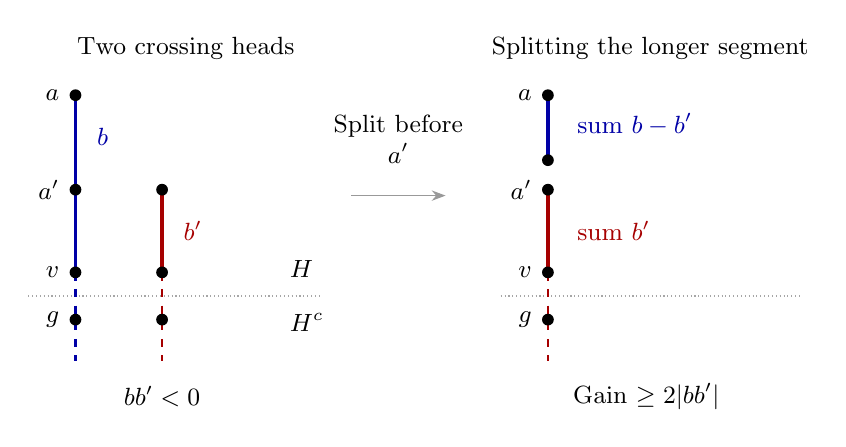
\begin{tikzpicture}[x=1cm,y=0.75cm,font=\small,
  head/.style={line width=1.4pt,blue!65!black},
  second/.style={line width=1.4pt,red!65!black},
  tail/.style={dashed,line width=1pt},
  vertex/.style={circle,fill=black,inner sep=1.5pt}]
  \node at (1.4,4.6) {Two crossing heads};
  \draw[gray!70,densely dotted] (-0.6,0.4)--(3.1,0.4);
  \node[anchor=west] at (2.6,0.85) {\(H\)};
  \node[anchor=west] at (2.6,-0.05) {\(H^c\)};
  \draw[head] (0,3.8)--(0,0.8);
  \draw[head,tail] (0,0.8)--(0,-0.7);
  \draw[second] (1.1,2.2)--(1.1,0.8);
  \draw[second,tail] (1.1,0.8)--(1.1,-0.7);
  \node[vertex,label=left:\(a\)] at (0,3.8) {};
  \node[vertex,label=left:\(a'\)] at (0,2.2) {};
  \node[vertex] at (1.1,2.2) {};
  \node[vertex,label=left:\(v\)] at (0,0.8) {};
  \node[vertex] at (1.1,0.8) {};
  \node[vertex,label=left:\(g\)] at (0,0) {};
  \node[vertex] at (1.1,0) {};
  \node[anchor=west,text=blue!65!black] at (0.15,3.1) {\(b\)};
  \node[anchor=west,text=red!65!black] at (1.25,1.5) {\(b'\)};
  \node at (1.1,-1.3) {\(bb'<0\)};
  \draw[-{Stealth[length=5pt]},gray!80] (3.5,2.1)--(4.7,2.1);
  \node[align=center] at (4.1,3.05) {Split before\\\(a'\)};
  \begin{scope}[xshift=6cm]
    \node at (1.3,4.6) {Splitting the longer segment};
    \draw[gray!70,densely dotted] (-0.6,0.4)--(3.2,0.4);
    \draw[head] (0,3.8)--(0,2.7);
    \draw[second] (0,2.2)--(0,0.8);
    \draw[second,tail] (0,0.8)--(0,-0.7);
    \node[vertex,label=left:\(a\)] at (0,3.8) {};
    \node[vertex] at (0,2.7) {};
    \node[vertex,label=left:\(a'\)] at (0,2.2) {};
    \node[vertex,label=left:\(v\)] at (0,0.8) {};
    \node[vertex,label=left:\(g\)] at (0,0) {};
    \node[anchor=west,text=blue!65!black] at (0.25,3.3)
      {sum \(b-b'\)};
    \node[anchor=west,text=red!65!black] at (0.25,1.5)
      {sum \(b'\)};
    \node at (1.25,-1.3) {Gain \(\ge2|bb'|\)};
  \end{scope}
\end{tikzpicture}
\caption{Opposite $p$-sums at a gate $g$, with $p$ supported in $H$.
The two heads on the left belong to different segment families;
their traces are displaced to show their nesting on the same ancestral
chain. Their tails are schematic and need not coincide.
On the right, the longer segment is split before $a'$; the lower
piece retains that segment's original tail and has $p$-sum $b'$.
The squared segment test increases by at least $2|bb'|$.}
\label{fig:opposite-crossing}
\end{figure}


Do this at every opposite-sign gate, in the family with the longer
head. Within each family each original segment is cut at most once,
because it crosses only one gate. Disjointness is preserved, so the
total gain in each family is at most its deficit $L$. Summing proves
\eqref{eq:opposite-crossing}.
\end{proof}


\section{Keeping the coefficient and slack budgets together}
\label{mol:sec:joint-budget}

We will replace each atom coefficient by a multiple of the head test's
sum on that segment. This produces two nonnegative errors: the squared
change of coefficients and the unused squared head-test energy. Their
sum is controlled by the squared-radius deficit of the center. Keeping
this joint budget proves the main estimate for the part of an arbitrary
displacement outside the head.

We use the segment atoms, ancestral projections, and cone decomposition
already established above.  The argument applies both to the coordinate
completion on the infinite tree and to the finite-height forest, after
their respective atomic-ball identifications.  It does not identify those
two spaces.



\begin{proof}[Proof of Theorem~\ref{thm:main-tail}]
Put $r=\|x\|$. If $r=0$, contractivity gives
$\|Q_Hy\|\le\|y\|\le R$, which proves the assertion. Assume $r>0$.
First suppose that $y$ has finite support, and enlarge $H$ to a finite
ancestral set $K$ containing that support.  Choose a head test $p$ of
norm one such that $x(p)=r$.  By the finite atomic-ball formula, choose
finite laws of represented vectors
\[
 A=\sum_i a_i d_{S_i},\qquad \sum_i a_i^2\le R^2,
\]
with means $x+y$ and $x-y$.  Choose a sign $\sigma$ with equal
probabilities and then the corresponding law.  Thus
$\mathbb EA=x$ and $\mathbb E(\sigma A)=y$.

For each outcome put
\[
 b_i=r p(S_i),\quad
 A^\circ=\sum_i b_i d_{S_i},\quad
 V=\sum_i(a_i-b_i)^2,\quad
 L=r^2-\sum_i b_i^2.
\]
Both $V$ and $L$ are nonnegative.  Since
$\mathbb E\sum_i a_i b_i=r\mathbb EA(p)=r^2$, expansion gives
\begin{equation}\label{mol:eq:joint-identity}
 \eta+\theta
 :=\mathbb EV+\mathbb EL
 =\mathbb E\sum_i a_i^2-r^2
 \le R^2-r^2.
\end{equation}
The atom coefficient estimate also gives
$\|Q_H(A-A^\circ)\|\le\sqrt V$.

Let $G$ be the gates outside $H$ which occur in the finite
representations.  At a gate $g$, write $b(g)$ for the coefficient of the
crossing segment in $A^\circ$, and put it equal to zero when there is
no crossing segment.  Every segment wholly outside $H$ has replaced
coefficient zero.  If $W=Q_H(A-A^\circ)$, then
\[
 \sum_{g\in G}|W(e_g)|^2\le V.
\]
Indeed, the gates are incomparable, so each segment contains at most
one gate, and disjointness assigns different gates to different
coefficients.  Since $\mathbb EA(e_g)=x(e_g)=0$,
\begin{equation}\label{mol:eq:joint-signed-mass}
 \sum_g(\mathbb Eb(g))^2
 =\sum_g(\mathbb EW(e_g))^2\le\mathbb EV=\eta.
\end{equation}

The simultaneous opposite-head splitting argument, applied to the
test $rp$, gives for two independent outcomes
\[
 2\sum_{g:b(g)b'(g)<0}|b(g)b'(g)|\le L+L'.
\]
Here the available squared-test budget is $r^2$; this is the only
change from the norm-one version.  Consequently, with
$m(g)=\mathbb E|b(g)|$,
\begin{equation}\label{mol:eq:joint-absolute-mass}
 \|m\|_2^2-\|\mathbb Eb\|_2^2
 =\mathbb E\sum_g\bigl(|b(g)b'(g)|-b(g)b'(g)\bigr)
 \le2\theta.
\end{equation}
Equations \eqref{mol:eq:joint-signed-mass} and
\eqref{mol:eq:joint-absolute-mass} therefore give
$\|m\|_2\le\sqrt{\eta+2\theta}$.

On the cone rooted at $g$, each replaced outcome is $b(g)d_{J(g)}$,
where $J(g)$ is its crossing tail starting at $g$.  The term is zero
when there is no crossing segment.  Thus the signed mean decomposes as
\begin{equation}\label{mol:eq:signed-product-recovery}
 Q_H\mathbb E(\sigma A^\circ)
 =\sum_g\mathbb E\bigl[\sigma b(g)d_{J(g)}\bigr].
\end{equation}
Each cone term has norm at most $\mathbb E|b(g)|=m(g)$, since
$|\sigma|=1$ and a segment indicator has norm one.  The cone identity
therefore gives
\[
 \|Q_H\mathbb E(\sigma A^\circ)\|
 \le\|m\|_2\le\sqrt{\eta+2\theta}.
\]
Lemma~\ref{stab:coef:tail-assembly} gives a direct convex-product proof
of the same reconstruction, allowing any multiplier of absolute value
at most one in place of $\sigma$.

The signed mean of the original atoms is $y$, so its tail satisfies
\[
 \|Q_Hy\|\le\sqrt\eta+\sqrt{\eta+2\theta}
 \le2\sqrt{\eta+\theta}.
\]
For the last inequality, square both sides and use
$\sqrt{\eta(\eta+2\theta)}\le\eta+\theta$.
Now apply \eqref{mol:eq:joint-identity}.

For an arbitrary completed vector $y$, take an increasing finite ancestral
exhaustion $K_n\supset H$.  Contractivity gives
$\|x\pm P_{K_n}y\|\le R$, and $P_{K_n}y\to y$ in norm.
The finite estimate passes to the limit.  No bound on the height or
the number of children entered the calculation.
\end{proof}

\section{Asymptotic midpoint growth}\label{sec:consequences}

The main tail estimate gives a uniform increase in the endpoint norms
on a finite-codimensional subspace. We specify the two standard
midpoint moduli before deriving this consequence for both models.

For an infinite-dimensional real Banach space $Y$ and $t>0$, define
the maximum-based asymptotic midpoint modulus by
\begin{equation}\label{eq:max-modulus}
 \overline\theta_Y(t)=\inf_{\|x\|=1}
 \sup_{F\in\operatorname{cof}(Y)}
 \inf_{y\in F,\,\|y\|=1}
 \left(\max\{\|x+ty\|,\|x-ty\|\}-1\right),
\end{equation}
where $\operatorname{cof}(Y)$ denotes the closed finite-codimensional
subspaces. This is the convention of \cite[Definition~2.2]{DKRRZ2016}.
A norm is AMUC when this modulus is positive for every $t>0$.

We shall also use the averaged convention
\begin{equation}\label{eq:averaged-modulus}
 \widehat\delta_Y(t)=\inf_{\|x\|=1}\sup_{F\in\operatorname{cof}(Y)}
 \inf_{y\in F,\,\|y\|=1}
 \left(\frac{\|x+ty\|+\|x-ty\|}{2}-1\right).
\end{equation}
For every infinite-dimensional real Banach space,
\begin{equation}\label{eq:modulus-comparison}
 \tfrac12\overline\theta_Y(t)\le\widehat\delta_Y(t)
 \le\overline\theta_Y(t).
\end{equation}
The second inequality is pointwise. For the first, fix a unit center
$x$ and a norming functional $f$. Intersect a finite-codimensional
subspace used for the maximum with $\ker f$. Both signed norms are then
at least one, and an excess $a$ for their maximum gives an excess at
least $a/2$ for their average. Arbitrary approximations to the supremum
over subspaces, followed by the infimum over centers, prove the first
inequality. The two conventions therefore agree as qualitative
properties, but their numerical bounds must be distinguished.

For either symmetric expression, allowing $\|y\|\ge1$ in place of
$\|y\|=1$ does not change the inner infimum. Indeed, the maximum and
the average are even convex functions of the scalar multiplying a fixed
direction, and are nondecreasing on the nonnegative half-line. This also
shows that both moduli are nondecreasing in $t$.

\subsection{Averaged midpoint growth at every radius}

Write $\widehat\delta(t)$ for the averaged modulus of the chosen
space, defined in \eqref{eq:averaged-modulus}.

\begin{corollary}\label{mol:cor:all-radius-averaged}
In either of the segment-atomic completions considered above,
\begin{equation}\label{mol:eq:all-radius-averaged}
 \widehat\delta(t)\ge
 \frac{\sqrt{1+t^2/4}-1}{2}\qquad(t>0).
\end{equation}
\end{corollary}

\begin{proof}
For a unit $x=P_Hx$ and $y\in\ker P_H$ with $\|y\|\ge1$,
Theorem~\ref{mol:prop:joint-budget} applied to $ty$ gives
\[
 \max\{\|x+ty\|,\|x-ty\|\}\ge\sqrt{1+t^2/4}.
\]
Both endpoint norms are at least one, by applying the contractive
projection $P_H$.  Their average therefore exceeds one by at least
the right side of \eqref{mol:eq:all-radius-averaged}.

For an arbitrary unit center $x$, choose a finitely supported unit
vector $x_0$ with $\|x-x_0\|<\varepsilon$, and let $H$ contain
its ancestral support.  The estimate for $x_0$ applies to every
$y\in\ker P_H$ of norm at least one.  Replacing $x_0$ by $x$
loses at most $\varepsilon$ in the average.  Take the infimum over
these $y$, then the supremum over finite-codimensional subspaces,
and finally let $\varepsilon\downarrow0$.  The resulting bound
is uniform over the original unit center.
\end{proof}


\section{Coordinate variants and bounded paths}\label{sec:coordinate-variants}
\subsection{Projections and height conventions}

The coordinate arguments also apply to restrictions of the forest and
to other choices of finite component heights. We first record these
variants, then use bounded root paths to rule out an equivalent AUC norm.

\begin{lemma}\label{foundation:order-convex}
Let $E$ be a set of vertices whose intersection with every segment is
empty or a segment. The coordinate projection $P_E$ is contractive on
both $J$ and $X=J^*$. Its range on $J$ is the completion of $c_{00}(E)$
under the segment norm restricted to $E$, and
\[
 \|P_Ex\|=\|x|_{P_EJ}\| \qquad (x\in X).
\]
In particular these assertions apply to an ancestral set, its
complement, a difference of nested ancestral sets, a descendant subtree,
and an antichain. On an antichain the coordinate norm on either space
is exactly the usual $\ell_2$ norm.
\end{lemma}
\begin{proof}
For a finite vector $u$, each segment sum of $P_Eu$ is the sum of $u$
over the intersection of that segment with $E$. Nonempty intersections
are disjoint segments when the original segments are disjoint. Taking
the supremum proves $\rho(P_Eu)\le\rho(u)$. Extend by density and take
the adjoint to obtain the assertion on $X$. Contractivity and density
identify $P_EJ$ with the indicated completion. Since $P_E$ maps the
unit ball of $J$ onto the unit ball of its range, restriction has exactly
the asserted dual norm. A segment meets an antichain in at most one
vertex; singleton tests then give the $\ell_2$ norm on its primal range.
The restriction identity and $\ell_2$ duality give the dual assertion.
\end{proof}

\begin{proposition}\label{foundation:height-variants}
Let $I$ be countable and let $(h_i)_{i\in I}$ be nonnegative integers.
On the disjoint forest
\[
 \mathcal F_{\boldsymbol h}
   =\coprod_{i\in I}(\{i\}\times\mathbb N^{\le h_i})
\]
define $J_{\boldsymbol h}$ by the same disjoint-segment norm and set
$X_{\boldsymbol h}=J_{\boldsymbol h}^*$. If $J(h)$ denotes the
single-tree completion on $\mathbb N^{\le h}$, then
\[
 J_{\boldsymbol h}
   =\Big(\bigoplus_{i\in I}J(h_i)\Big)_{\ell_2},
 \qquad
 X_{\boldsymbol h}
   =\Big(\bigoplus_{i\in I}J(h_i)^*\Big)_{\ell_2}
\]
isometrically under coordinate restriction. Both spaces are reflexive,
and finite coordinate vectors are dense in each. The projection and
complementary-subtree formulas remain valid for this forest.

The convention of one tree with $n$ levels, including the root, for
every $n\ge1$ gives exactly
\[
 J_{\mathrm{levels}}=\mathbb R\oplus_2 J,
 \qquad X_{\mathrm{levels}}=\mathbb R\oplus_2 X.
\]
Its component estimate is
$\|u\|_2\le\rho(u)\le\sqrt n\,\|u\|_2$, and a root-to-leaf path
has $n-1$ extension steps.
\end{proposition}
\begin{proof}
Every segment belongs to one component. Grouping a test family by
component gives one inequality in the primal sum formula. For the
other, choose nearly maximizing finite families on each of the
finitely many components meeting the support and combine them.
Completion gives the displayed primal identity, and duality for
$\ell_2$ sums gives the dual identity. On component $i$,
\[
 \|u\|_2\le\rho(u)\le\sqrt{h_i+1}\,\|u\|_2.
\]
Thus each component and its dual are reflexive Hilbert space
renormings with dense coordinates. The sum identities give
reflexivity and coordinate density on the entire forest. No bound
uniform in $i$ on the Hilbert space comparison is needed. Projection
contractivity uses only segment intersection, as in
Lemma~\ref{foundation:order-convex}; the complementary-subtree identity
uses independent segment tests in its incomparable subtrees.

For the last assertion, put $h=n-1$. The component $n=1$ is the
one-dimensional singleton tree with the absolute-value norm. The
remaining components have heights $1,2,\ldots$, and the coordinate map
$(n,\sigma)\mapsto(n-1,\sigma)$ preserves their segments and all their
tests. Splitting off the singleton proves both isometries. The
component bound and the number of extension steps follow from the
maximal chain cardinality $n$.
\end{proof}

\subsection{Bounded paths and equivalent norms}

A single segment functional has norm one even when the segment is very
long. Its successive coordinate increments therefore give bounded
paths. The following argument explains why weakly null choices of the
next increment obstruct an asymptotically uniformly convex equivalent
norm. It also retains the precise radius when increments are normalized
before being approximated in a finite-codimensional subspace.

For a norm $N$ on an infinite-dimensional real Banach space $Z$, write
$S_N=\{z:N(z)=1\}$ and let $\operatorname{cof}(Z)$ denote the closed
finite-codimensional linear subspaces. Define
\begin{equation}\label{eq:one-sided-modulus}
 \overline\delta_N(t)=\inf_{x\in S_N}
   \sup_{F\in\operatorname{cof}(Z)}
   \inf_{y\in F\cap S_N}\bigl(N(x+ty)-1\bigr),\qquad t>0.
\end{equation}
Positivity at every $t>0$ is asymptotic uniform convexity.
The spheres $F\cap S_N$ are nonempty. A norming functional for $x$,
with $F$ contained in its kernel, gives the lower bound in
$0\le\overline\delta_N(t)\le t$; the upper bound is the triangle
inequality.

\begin{lemma}\label{foundation:weak-null-growth}
Let $x\in S_N$, let $(z_j)$ be weakly null, and suppose $N(z_j)\ge t>0$
for every $j$. For every
$0<\gamma<\overline\delta_N(t)$, all sufficiently large $j$ satisfy
\[
 N(x+z_j)>1+\gamma.
\]
\end{lemma}
\begin{proof}
Choose $\eta$ with $\gamma<\eta<\overline\delta_N(t)$ and then
$F\in\operatorname{cof}(Z)$ such that
$N(x+tv)>1+\eta$ for every $v\in F\cap S_N$.
Put $u_j=z_j/N(z_j)$. These vectors are weakly null because
$1/N(z_j)\le1/t$. Their images in $Z/F$ converge to zero weakly,
hence in norm, since the quotient is finite dimensional. Choose
$v_j\in F$ with $N(v_j-u_j)\to0$. Then $N(v_j)\to1$, so
$w_j=v_j/N(v_j)$ is defined for large $j$, belongs to $F\cap S_N$,
and satisfies $N(w_j-u_j)\to0$. Consequently
\[
 N(x+t u_j)>1+\eta-tN(w_j-u_j)>1+\gamma
\]
for large $j$. For $r\ge t$, convexity gives
\[
 N(x+r u_j)-1\ge\frac rt\bigl(N(x+t u_j)-1\bigr).
\]
Apply this at $r=N(z_j)$ to finish the proof.
\end{proof}

There is a second useful form of the approximation step. If
$N(z_j)\ge2t$ and $N(x+tv)>1+\eta$ on $F\cap S_N$, approximate
$z_j$ directly by $v_j\in F$ with $N(z_j-v_j)\to0$.
Eventually $N(v_j)\ge t$, so the same ray-convexity inequality gives
$N(x+v_j)>1+\eta$. For every $0<\gamma<\eta$, choosing
$N(z_j-v_j)<\eta-\gamma$ gives $N(x+z_j)>1+\gamma$.
This form uses the spare factor two in the radius and does not require
approximating the normalized sequence.

\begin{proposition}\label{foundation:bounded-tree}
Suppose an infinite-dimensional real Banach space $(Z,\|\cdot\|)$
contains, for every positive
integer $k$, vectors $(u_s)_{s\in\mathbb N^{\le k}}$ such that
\[
 0<m\le\|u_s\|\le M,
 \qquad \|u_{s^\frown j}-u_s\|\ge c>0,
\]
where $m,M,c$ are independent of $k$, and for each nonterminal $s$ the
sequence $(u_{s^\frown j}-u_s)_j$ is weakly null against the whole
continuous dual of $Z$. If
$0<a\le b<\infty$ and $a\|z\|\le N(z)\le b\|z\|$, then
\[
 \overline\delta_N\!\left(\frac{ac}{bM}\right)=0.
\]
In particular the same conclusion holds at $ac/(2bM)$, and $Z$ admits
no equivalent asymptotically uniformly convex norm.
\end{proposition}
\begin{proof}
Suppose the modulus at $t=ac/(bM)$ is positive and choose
$0<\gamma<\overline\delta_N(t)$. At a nonterminal $s$, put
\[
 x=\frac{u_s}{N(u_s)},\qquad
 z_j=\frac{u_{s^\frown j}-u_s}{N(u_s)}.
\]
The equivalent norms have the same continuous linear functionals,
so $(z_j)$ is weakly null, and $N(z_j)\ge ac/(bM)=t$.
Lemma~\ref{foundation:weak-null-growth} gives a child for which
$N(u_{s^\frown j})>(1+\gamma)N(u_s)$. Starting at the root and
repeating $k$ times gives $am(1+\gamma)^k<bM$, which is impossible
for sufficiently large $k$. Thus the modulus at $t$ is zero. Applying
the same argument at $t/2$, using either the lemma or the direct
approximation form above, proves the stated smaller-radius conclusion.
\end{proof}

\begin{corollary}\label{foundation:forest-obstruction}
If the finite component heights $h_i$ in
Proposition~\ref{foundation:height-variants} are unbounded, then every
equivalent norm $N$ on $X_{\boldsymbol h}$ with
$a\|x\|\le N(x)\le b\|x\|$ satisfies
\[
 \overline\delta_N(a/b)=\overline\delta_N(a/(2b))=0.
\]
\end{corollary}
\begin{proof}
For a vertex $s$ in a component with root $o$, put
$u_s=\sum_{o\preceq v\preceq s}e_v^*$. A single segment test gives
$\|u_s\|\le1$, while evaluation on $e_s$ gives equality. Likewise
$\|e_s^*\|=1$, and
$u_{s^\frown j}-u_s=e_{s^\frown j}^*$.
These increments are weakly null: under the canonical identification
$X_{\boldsymbol h}^*=J_{\boldsymbol h}$, their evaluations on $g$
are the coordinates $g(s^\frown j)$, which tend to zero since
$\|g\|_2\le\rho(g)$. Equivalently, the coordinate map on this fixed
component is a Hilbert space isomorphism, so every continuous
functional on the full space restricts to a continuous Hilbert space
functional there. Components of unbounded finite height give the
trees required by Proposition~\ref{foundation:bounded-tree}, with
$m=M=c=1$. For the convention of $n$ levels the same iteration makes
$n-1$ steps. Both step counts tend to infinity.
\end{proof}

\section{The infinite-height renorming obstruction}\label{sec:infinite-obstruction}
\begin{proposition}[The bounded-path obstruction]\label{binf:obstruction}
The unit root-path vectors in $B_\infty$ have unit child increments
which are weakly null among the children of each fixed vertex. Every
sequence of distinct coordinate vectors is in fact weakly null.
If $a\|\cdot\|\le N\le b\|\cdot\|$, with $0<a\le b<\infty$,
then the one-sided asymptotic modulus of $N$ vanishes at $a/(2b)$
and at $a/b$. In particular, $B_\infty$ has no equivalent AUC norm.
The same obstruction holds for the finite-height forest, using trees
of arbitrarily large finite height.
\end{proposition}
\begin{proof}
Singleton tests and Cauchy--Schwarz give
\[
 \left\|\sum_v c_v e_v^*\right\|\le
 \left(\sum_v c_v^2\right)^{1/2}.
\]
For coefficients supported on an antichain, equality holds: the test
with proportional coefficients on that antichain has its Euclidean
norm, since a segment meets it in at most one point. In particular
sibling coordinate vectors span an isometric $\ell_2$.
Thus the map sending the unit vectors of $\ell_2(T_\infty)$ to
$e_v^*$ extends boundedly into $B_\infty$. For any $L\in B_\infty^*$,
finite Euclidean duality gives
$\sum_v|L(e_v^*)|^2\le\|L\|^2$. Hence distinct coordinates are
weakly null against the whole continuous dual. A root-path functional
$z_v=d_{[o,v]}$ has norm one, by the single segment upper bound and
any coordinate test on that path. Its child is
$z_{v^\frown n}=z_v+e_{v^\frown n}^*$.

Use the one-sided modulus defined in \eqref{eq:one-sided-modulus}.
It is nonnegative: for each $x$, the kernel of a norming functional
makes every displayed norm at least one. Suppose its value is positive
at a radius $r_0\le a/b$. Choose $0<d<\overline\delta_N(r_0)$.
For a path $z$, put $x=z/N(z)$ and choose $F$ so that
$N(x+r_0w)\ge1+d$ on the $N$-unit sphere of $F$. The normalized
child directions $v_n=e_{v^\frown n}^*/N(e_{v^\frown n}^*)$ are
weakly null. Their images in the finite-dimensional quotient by $F$
converge to zero in norm. Approximate them in $F$ and normalize those
approximants to obtain $N$-unit vectors $w_n\in F$ with
$N(v_n-w_n)\to0$. Choose $N(v_n-w_n)<d/(2r_0)$. Then
$N(x+r_0v_n)>1+d/2$ for large $n$. The actual child step has radius
\[
 r_n=\frac{N(e_{v^\frown n}^*)}{N(z)}\in[a/b,b/a].
\]
Convexity along this ray, including the case $r_n=r_0$, gives
\begin{equation}\label{binf:radial-growth}
 N(x+r_nv_n)>1+\frac{r_n}{r_0}\frac d2\ge1+\frac d2.
\end{equation}
Choosing a child repeatedly contradicts $a\le N(z_v)\le b$.
For the forest, choose the component height in advance large enough
that $a(1+d/2)^h>b$ and carry out only $h$ such selections.

\end{proof}

\subsection{Transferring the cofinite gain to a child}
\label{binf:transfer-comparisons}

The following procedures keep track of the radius and approximation error
in the bounded-path argument. Fix the equivalent norm $N$ and constants
$a,b$ from Proposition~\ref{binf:obstruction}. For a root path
$z=d_{[o,v]}$, put $x=z/N(z)$ and write $e_n=e_{v^\frown n}^*$
for its child increments. Then
\[
 a\le N(z)\le b,\qquad a\le N(e_n)\le b.
\]
At each stated radius $r_0$, suppose a finite-codimensional subspace $F$
gives $N(x+r_0w)\ge1+d$ for every $N$-unit $w\in F$, with $d>0$
chosen below the putative positive modulus. Raw, path-normalized, and
unit child sequences are weakly null, so all three can be approximated
in $F$. Each resulting uniform child gain contradicts bounded path norms
by the iteration just proved.

\paragraph{Raw children at the safety radius.}
At the safety radius $r_0=a/(2b)$, one can approximate the child
without first normalizing it.
Given a cofinite gain $d>0$ at $z/N(z)$, choose a raw child $e$ and
$q\in F$ with
\begin{equation}\label{binf:raw-error}
 N(e-q)<\min\{a/2,dN(z)/2\}.
\end{equation}
Then $N(q)\ge a/2\ge r_0N(z)$, and ray convexity yields
$N(z+q)\ge(1+d)N(z)$. Consequently
$N(z+e)\ge(1+d/2)N(z)$. The stronger restriction
$N(e-q)<\min\{a/2,ad/2\}$ suffices uniformly over all paths.
If the cofinite gain is $2d$, the error bound $dN(z)$ gives factor
$1+d$; if that gain is half a named modulus $\delta$, error less
than $\delta N(z)/4$ gives factor $1+\delta/4$.

\paragraph{Repair at the endpoint radius.}
Normalize a raw child by the path norm, setting
$h_n=e_{v^\frown n}^*/N(z)$. Its norm is at least $a/b$. At the
radius $r_0=a/b$, take $q_n\in F$ with $N(q_n-h_n)\to0$.
These approximants may have norm slightly less than $r_0$. For large
$n$, set
\begin{equation}\label{binf:radial-repair}
 q_n'=\max\{1,r_0/N(q_n)\}\,q_n.
\end{equation}
Since $N(h_n)\ge r_0$, the enlargement costs at most
$N(q_n-h_n)$, so $N(q_n'-h_n)\le2N(q_n-h_n)\to0$.
The cofinite gain applied to $q_n'$ therefore gives a strict child
factor greater than $1+d/2$ once the repaired error
$N(q_n'-h_n)$ is less than $d/2$ (for example, when the original
error is less than $d/4$).
At the safety radius $r_0=a/(2b)$ no enlargement is needed:
$N(h_n)\ge2r_0$, and choosing
$N(q_n-h_n)<\min\{r_0,\gamma/2\}$ transfers a cofinite gain
$\gamma$ to a strict child factor greater than $1+\gamma/2$.

\paragraph{Unit directions at the variable radius.}
For $0<r_0\le a/b$, the unit-child procedure from the proof inserts the
approximating unit direction at the actual variable radius $r_n$,
instead of first transferring at $r_0$. Ray convexity gives
$N(x+r_nw_n)\ge1+d$. As $r_n\le b/a$,
\begin{equation}\label{binf:variable-radius-transfer}
 N(x+r_nv_n)\ge1+d-r_nN(v_n-w_n)
              \ge1+d-(b/a)N(v_n-w_n)>1+d/2
\end{equation}
for all sufficiently close unit approximants. This proves the
variable-scale transfer with its uniform error factor and also covers
the endpoint $r_n=r_0$.

\paragraph{Additive growth.}
At the safety radius $r_0=a/(2b)$, a cofinite gain $\eta>0$ gives
$N(z+q)\ge N(z)+a\eta$ since $N(z)\ge a$. With
$N(e-q)<\min\{a/2,a\eta/2\}$, each chosen child satisfies
$N(z+e)\ge N(z)+a\eta/2$. Repetition again contradicts the same
upper bound $b$. This is a separate way to accumulate the gain.

\subsection{Parameter choices for the raw-child transfer}

At the safety radius $t_0=a/(2b)$, the raw-child argument above
turns a cofinite gain into growth of a root-path norm. The following
statement records three choices of that gain and their uniform error
bounds.

\begin{proposition}\label{stab:sign:obstruction}
In $B_\infty$, the root paths $h_v=d_{[o,v]}$ and the coordinates
$e_v^*$ have norm one, and the children $(e_{v^\frown j}^*)_j$ of
each fixed vertex are weakly null. If
$a\|z\|\le N(z)\le b\|z\|$, with $0<a\le b<\infty$, then
$\overline\delta_N(a/(2b))=0$.

More precisely, put $t_0=a/(2b)$, with $d,\varepsilon>0$ below.
Each of the following assumptions
would permit a finite-codimensional subspace and a child whose
approximation error and growth factor satisfy the corresponding row:
\[
\begin{array}{c|c|c}
 \text{assumed positive lower bound}&
 \text{error less than}&\text{growth factor}\\\hline
 0<d<\overline\delta_N(t_0)&\min(a/2,ad/2)&1+d/2\rule{0pt}{13pt}\\
 2\varepsilon<\overline\delta_N(t_0)&
       \min(a/2,a\varepsilon/2)&1+\varepsilon/2\\
 d=\overline\delta_N(t_0)>0&\min(a/2,ad/4)&1+d/4
\end{array}
\]
Here the error is $N(e_v^*-f)$ for the chosen child and its
approximant $f$ in the finite-codimensional subspace. Growth is
measured relative to the $N$-norm of the parent root-path vector.
\end{proposition}

\begin{proof}
The path norms, weak nullity against the whole dual and vanishing
one-sided modulus are Proposition~\ref{binf:obstruction}.
For the table, choose respectively a cofinite gain
$\gamma=d$, $\gamma=\varepsilon$ or $\gamma=d/2$.
The uniform raw-child error bound
$N(e_v^*-f)<\min(a/2,a\gamma/2)$ from
\eqref{binf:raw-error} gives growth at least $1+\gamma/2$.
These are exactly the three rows. In the last row the selected gain
$d/2$ lies strictly below the named modulus, as required by the
supremum over finite-codimensional subspaces.
\end{proof}


\begin{remark}[Taking the supremum of the path norms]\label{binf:supremum-obstruction}
For the infinite tree there is a second contradiction that uses no
iteration along a branch. Set
\[
 M=\sup_v N(d_{[o,v]})\in[a,b],\qquad t_0=\frac{a}{2M}.
\]
Suppose $0<\gamma<\overline\delta_N(t_0)$. For each path vector
$z=d_{[o,v]}$, choose a cofinite subspace $F$ giving gain $\gamma$
at $z/N(z)$. The child increments $e_{v^\frown n}^*$ are weakly
null, so choose $q_n\in F$ with
$N(q_n-e_{v^\frown n}^*)\to0$. Eventually
$N(q_n)\ge a/2\ge t_0N(z)$. Convexity along the ray through $q_n$
therefore gives $N(z+q_n)\ge(1+\gamma)N(z)$. Passing to the lower
limit and using the vanishing approximation error yields
\[
 M\ge\liminf_n N(z+e_{v^\frown n}^*)\ge(1+\gamma)N(z).
\]
Taking the supremum over all $v$ gives $M\ge(1+\gamma)M$, a
contradiction. No path is required to attain $M$. This argument uses
the fact that every vertex of the infinite tree has children; the
finite-height forest is covered by the finite-iteration argument above.
\end{remark}

\section{Clipping cumulative segment sums}\label{clip:section}

We now perturb a primal head test while keeping the squared cost
quadratic in the perturbation size. The construction works on
$T_\infty$ and on the finite-height forest. In this section $\mathcal T$
denotes either tree system, $J(\mathcal T)$ its segment completion,
and $Z$ its closed coordinate span in $J(\mathcal T)^*$. Thus
$Z=B_\infty$ in the first case and $Z=X$ in the second. We retain
$\rho$ for the test norm and $\|\cdot\|$ for the coefficient norm.
All tests constructed below are finitely supported.

Fix a finite ancestral head $H$. For a gate $g$ let $U_g$ be its
exterior cone, and give its parent the artificial cumulative value zero
when that parent is absent from the component. For $v=Q_Hv$ define
\[
 V_g(w)=v([g,w]),\qquad
 m_g=\max_{w\in U_g}|V_g(w)|,\qquad
 q_g=\rho(v\mathbf1_{U_g}).
\]
These maxima exist: finite support gives only finitely many distinct
cumulative values. We have
\begin{equation}\label{clip:budgets}
 \sum_gm_g^2\le\rho(v)^2=\sum_gq_g^2.
\end{equation}
The equality follows from the exterior square-sum identity. For the
inequality, choose one maximizing root prefix in each nonzero cone;
these prefixes are disjoint.

A third useful grouping collects cones with the same last head vertex.
For $p\in H$, let $C_p$ consist of all exterior vertices whose last
ancestor in $H$ is $p$. Either of
\begin{equation}\label{clip:group-budgets}
 b_p=\rho(v\mathbf1_{C_p}),\qquad
 M_p=\max_{w\in C_p}|v((p,w])|
\end{equation}
may be used as its budget, with $M_p=0$ when $C_p$ is empty. Both satisfy
$\sum_pb_p^2\le\rho(v)^2$ and $\sum_pM_p^2\le\rho(v)^2$.
The first follows by joining nearly maximizing families in the disjoint
regions; for the second choose one maximizing prefix in each region.
A region may contain several cones, but a segment meeting it stays
in one cone, and disjoint crossing segments have distinct last head
vertices. These facts, rather than an assumed orthogonality within a
region, justify the grouping. For a component disjoint from $H$, there is no
last head vertex. Keep each such cone as a separate group, use its
prefix maximum or full cone norm, and choose an arbitrary fixed
inward sign. It has no head crossing and contributes only to exterior
squares. This convention also handles $H=\varnothing$.

\begin{lemma}[An inward crossing estimate]\label{clip:crossing}
Let $f=P_Hf$ and $v=Q_Hv$ be finite tests. Use either the cone budgets
$m_g$ or $q_g$, or the last-head budgets in
\eqref{clip:group-budgets}; write $c_j$ for the chosen budget of a
cone or region. Fix $s>0$. At each attached group choose the shortest
head suffix ending at its attachment whose $f$-sum has magnitude at
least $sc_j$, if one exists and $c_j>0$. Let $\sigma_j$ be the
opposite sign of that sum, and otherwise choose either sign.

Suppose a finite exterior test $w$ satisfies
$\rho(w)\le\rho(v)$, and every root prefix in group $j$ has
$w$-sum in $\sigma_j[0,c_j]$. Then
\begin{equation}\label{clip:crossing-bound}
 \rho(f+sw)^2\le\rho(f)^2+3s^2\rho(v)^2.
\end{equation}
The same conclusion holds with a strictly greater suffix threshold,
provided the small-crossing case includes equality. With a non-strict
suffix threshold, equality may also be assigned to the small-crossing
case, leaving only strictly larger terms to be split.
\end{lemma}
\begin{proof}
Take a disjoint segment family. Write $A_i$ and $B_i$ for its head
$f$-sum and exterior $w$-sum. Then
$\sum_iB_i^2\le\rho(v)^2$. A positive product $A_iB_i$ occurs
only at a crossing, and different crossings use different cone indices
(or different last head vertices in the grouped construction).
If $|A_i|<sc_j$, its cross term is bounded by $2s^2c_j^2$.
Their total is at most $2s^2\rho(v)^2$.

For a remaining positive product, the head qualifies for the suffix
selection. It contains the selected suffix, whose sum $C_i$ has the
opposite sign to $A_i$ and magnitude at least $sc_j$. The suffix is
proper, so splitting it off leaves two nonempty head segments. The
increase in their squared $f$-sums is
\begin{equation}\label{clip:split-gain}
 (A_i-C_i)^2+C_i^2-A_i^2
 =2C_i^2-2A_iC_i\ge2s|A_i|c_j\ge2sA_iB_i.
\end{equation}
These cuts are simultaneous cuts in distinct original segments.
Their pieces and the other nonempty heads are a valid disjoint test
family for $f$. Thus the original head energy plus all large positive
cross terms is at most $\rho(f)^2$. Drop nonpositive cross terms,
add the small-crossing budget $2s^2\rho(v)^2$, and add the pure
exterior budget $s^2\rho(v)^2$. This proves the result.
For a strict threshold, use $|A_i|\le sc_j$ in the small case and
$|A_i|>sc_j$ in the large case; the proof is unchanged.
\end{proof}

\begin{lemma}[Two cumulative clips]\label{clip:two-clips}
For every $s>0$ and finite tests $f=P_Hf$, $v=Q_Hv$, there are
$h_1,h_2$ supported on $\operatorname{supp}v$ such that
\begin{equation}\label{clip:difference-split}
 v=h_1-h_2,\qquad \rho(h_j)\le\rho(v),\qquad
 \rho(f+sh_j)^2\le\rho(f)^2+3s^2\rho(v)^2\quad(j=1,2).
\end{equation}
Equivalently, $v=k_1+k_2$ with $k_1=h_1$, $k_2=-h_2$, and the
two admissible perturbations are $f+sk_1$ and $f-sk_2$.
\end{lemma}
\begin{proof}
Fix any one of the budgets above and choose its signs by
Lemma~\ref{clip:crossing}. For each group let
$\Phi_j(r)=\sigma_j\max\{\sigma_j r,0\}$. On an exterior cone
in that group, set the cumulative potentials of $h_1,h_2$ equal to
$\Phi_j(V_g(w))$ and $\Phi_j(-V_g(w))$, respectively, and take
successive differences down the edges from initial value zero.
Since $\Phi_j(r)-\Phi_j(-r)=r$, the difference of the two tests
is $v$. If $v(w)=0$, its cumulative values at $w$ and its parent
are equal, so both new increments vanish. Thus no new support appears,
even along infinite descendant paths.

On any segment in a cone, its $h_j$-sum is a difference of two values
of a single $1$-Lipschitz map. Its magnitude is therefore at most the
absolute $v$-sum on that same segment. The same assertion holds for a
crossing after deleting its zero head portion. In a last-head group,
both endpoints use the same grouping index, including the artificial
zero at the head predecessor. Hence $\rho(h_j)\le\rho(v)$.
Root prefixes have the chosen sign and the chosen budget bounds their
magnitudes. Lemma~\ref{clip:crossing} completes the proof.
\end{proof}

The large-crossing calculation has a second form which retains only
one of the two split pieces. If $A_iC_i<0$, the preceding head piece
has sum $A_i-C_i$, and
\begin{equation}\label{clip:shortening}
 (A_i-C_i)^2\ge A_i^2+2s|A_i|c_j
                 \ge A_i^2+2sA_iB_i.
\end{equation}
Keeping this piece for each large crossing, and keeping each other
head unchanged, is again a disjoint head family. This proves the
homogeneous sum-decomposition estimate in
Lemma~\ref{clip:two-clips} by shortening rather than by retaining both
pieces. The missing suffix is discarded only from the test family,
not from the vector being constructed.

\subsection{What the two tests recover}\label{clip:testing}

For $x=P_Hx$ and $y\in\ker P_H$, the mixed head--tail pairings
vanish. If $\rho(f),\rho(v)\le1$, $x(f)=\|x\|$, and
$y(v)\ge\theta\|y\|$ for $0<\theta<1$, the two clips yield both
\begin{align}
 \max_\pm\|x\pm ty\|&\ge
 \frac{\|x\|+st\theta\|y\|/2}{\sqrt{1+3s^2}},
 \label{clip:max-testing}\\
 \frac{\|x+ty\|+\|x-ty\|}{2}&\ge
 \frac{\|x\|+st\theta\|y\|/2}{\sqrt{1+3s^2}}.
 \label{clip:paired-testing}
\end{align}
The first uses one clip with $|y(h_j)|\ge\theta\|y\|/2$ and
chooses the corresponding endpoint sign. The second tests $x+ty$ on
$f+sh_1$ and $x-ty$ on $f+sh_2$, and uses
$y(h_1)-y(h_2)=y(v)$ before averaging. These are distinct testing
procedures, although their displayed right sides agree. Both norms
are separately at least $\|x\|$ by testing on $f$.

Finite tail vectors have exact norming tests after a finite ancestral
projection and then $Q_H$. For completed tails, finite test density
allows $\theta\uparrow1$; alternatively approximate the tail in norm
using Lemma~\ref{binf:projections}. Thus, for every $s,t>0$,
\begin{equation}\label{clip:general-head-tail}
 \max_\pm\|x\pm ty\|\ge
 \frac{\|x\|+st\|y\|/2}{\sqrt{1+3s^2}}.
\end{equation}
This preserves arbitrary head norms and arbitrary tail magnitudes.
In particular, if $\|x-P_Hx\|<\varepsilon$ at a unit center and
$y\in\ker P_H$, $\|y\|\ge1$, contractivity gives both endpoint
bounds $\|x\pm ty\|\ge1-\varepsilon$, while
\eqref{clip:general-head-tail} applied to $P_Hx$ gives
\[
 \max_\pm\|x\pm ty\|\ge
 \frac{1-\varepsilon+st/2}{\sqrt{1+3s^2}}-\varepsilon.
\]

The paired argument also gives the same lower bound for the average.

Use the averaged modulus in \eqref{eq:averaged-modulus}, with $Z$
as the chosen coordinate space. A uniform estimate proved for finite unit centers passes to general
centers by normalized finite approximation. If its excess is $E(t)$,
choosing an approximation within $E(t)/2$ retains $E(t)/2$.
If approximation errors are allowed to tend to zero after choosing
the cofinite subspace, the full $E(t)$ remains. The supremum over
subspaces is taken before the infimum over centers. For a bound first
proved for unit tails, the symmetric norm average is an even convex
function of the tail radius, hence nondecreasing at nonnegative radii;
this gives the required $\|y\|\ge1$ version.

\begin{corollary}[The averaged clipping estimate]\label{clip:paired-modulus}
For the infinite-height coordinate predual $B_\infty$ and the
finite-height forest space $X$,
\[
 \widehat\delta_Z(t)\ge\sqrt{1+t^2/12}-1\qquad(t>0).
\]
\end{corollary}
\begin{proof}
Use the paired test procedure \eqref{clip:paired-testing}, let the
tail test approach its norm, and put $s=t/6$. At a finite unit center
the average is at least
\[
 \frac{1+st/2}{\sqrt{1+3s^2}}=\sqrt{1+t^2/12}.
\]
Arbitrarily close normalized approximation of the center preserves this
bound. The construction applies to untouched forest components because
they have no crossing terms. It needs no bound on the component height.
\end{proof}

\subsection{Homogeneous consequences of the clipped tests}
\label{dir:primal:add:homogeneous}
We record two consequences of the common clipped construction that
will be useful for comparing midpoint bounds. Here \(X\) is the finite-height
forest dual, and \(H\) is a finite ancestral head.

\begin{proposition}\label{dir:primal:add:head-tail-lens}
If \(x=P_Hx\) and \(y=Q_Hy\), then
\begin{equation}\label{dir:primal:add:optimized}
 \max_{\pm}\|x\pm y\|\ge\sqrt{\|x\|^2+\|y\|^2/12}.
\end{equation}
If \(0<\sigma\le1\) and \(w,Z_1,Z_2,\ldots\in X\) satisfy
\(\|w\pm Z_j\|\le1\) and \(\|Z_j-Z_l\|\ge2\sigma\) for \(j\ne l\),
then \(\|w\|\le1-\sigma^2/24\).
\end{proposition}
\begin{proof}
In \eqref{clip:general-head-tail}, put \(t=1\) and
\(s=\|y\|/(6\|x\|)\) when both vectors are nonzero. This gives
\eqref{dir:primal:add:optimized}. If \(y=0\) the assertion is equality;
if \(x=0\), it follows from \(\|y\|\ge\|y\|/\sqrt{12}\).

For the second assertion, given \(\varepsilon>0\), choose \(H\) with
\(\|w-P_Hw\|\le\varepsilon\). The bounded sequence \(P_HZ_j\) has two
distinct terms for which \(h=(Z_j-Z_l)/2\) satisfies
\(\|P_Hh\|\le\varepsilon\). Then \(\|h\|\ge\sigma\) and
\(\|w\pm h\|\le1\) by convexity. Formula~\eqref{clip:general-head-tail}
at \(P_Hw,Q_Hh\), again with \(t=1\), gives
\[
 (1+2\varepsilon)\sqrt{1+3s^2}
 \ge\|w\|-\varepsilon+\tfrac{s}{2}(\sigma-\varepsilon).
\]
Let \(\varepsilon\downarrow0\), put \(s=\sigma/6\), and use
\(\sqrt{1+3s^2}\le1+3s^2/2\). This retains the stated \(1/24\) loss.
\end{proof}

\subsection{Three ways to retain a useful sign}\label{clip:selection}

We return to both choices of $Z$ for the three selection procedures below.

The two global clips retain half the original pairing in a single
endpoint test. Sometimes the construction selects signs before it
chooses that endpoint. The resulting extra loss records a different
selection mechanism.

\begin{proposition}[Selection before testing]\label{clip:selection-prop}
Suppose $x=P_Hx$, $\|x\|=1$, $y\in\ker P_H$, and
$v=Q_Hv$, $\rho(v)\le1$, and $y(v)>\|y\|/2$.
For every $s>0$, each of
the following constructions produces an exterior test $w$ with
\[
 |y(w)|>\|y\|/8,\qquad \rho(w)\le1,
 \qquad \rho(f+sw)^2\le1+3s^2,
\]
where $f=P_Hf$ norms $x$ and the inward signs are chosen with full
cone budgets $q_g$.

\begin{enumerate}
\item Take the positive and negative cumulative parts globally, choose
one by its total pairing, then retain one of the two groups of cones
having the same prescribed inward sign.
\item Form all four combinations of a cumulative positive/negative
part and a prescribed inward-sign group, and select one by its pairing.
\item Choose a cumulative part separately in each cone, orient it
inward, then retain the cones on which the resulting pairings have
one common sign.
\end{enumerate}
\end{proposition}
\begin{proof}
The exterior-test requirement loses no norming accuracy: replacing any
finite test $v$ by $Q_Hv$ preserves $y(v)$ and cannot increase $\rho(v)$.
Let $v^+,v^-$ be the successive differences of $\max(V_g,0)$ and
$\max(-V_g,0)$ on each cone. Both have nonnegative root prefixes,
$v=v^+-v^-$, and each segment sum is dominated in absolute value
by the corresponding $v$-sum.

For the first construction choose $q\in\{v^+,v^-\}$ with
$|y(q)|>\|y\|/4$. Partition its cones by $\sigma_g=1$ and
$\sigma_g=-1$, writing $q=q_++q_-$. One part has pairing of
absolute value greater than $\|y\|/8$. For that sign $\sigma$
put $w=\sigma q_\sigma$. This last sign makes its root prefixes
inward; the eventual endpoint sign is chosen from the sign of $y(w)$.
These two choices must not be confused.

For the second construction form
$w_{\sigma,+}=\sigma v^+\mathbf1_{\{\sigma_g=\sigma\}}$ and
$w_{\sigma,-}=\sigma v^-\mathbf1_{\{\sigma_g=\sigma\}}$ for
$\sigma\in\{-1,1\}$. Then
$v=\sum_\sigma\sigma(w_{\sigma,+}-w_{\sigma,-})$.
The triangle inequality for their four pairings gives the claimed
$1/8$ bound for one of them. Each of the four was fixed before the
endpoint was selected.

For the third construction write $v_g=v\mathbf1_{U_g}$. In each
nonzero cone select $q_g'$ from the two cumulative parts so that
$|y(q_g')|\ge|y(v_g)|/2$. Reverse the selected part if necessary
to make its root prefixes inward. Call the oriented test $r_g$.
Then
\[
 \sum_g|y(r_g)|\ge\tfrac12\sum_g|y(v_g)|
                    \ge\tfrac12y(v)>\|y\|/4.
\]
Keep either the positive-pairing cones or the negative-pairing cones,
whichever has larger total absolute pairing, and sum their $r_g$.
This loses another factor two. The selected half in each cone can
differ; this procedure is not the choice of one of two fixed global
clips.

In all three constructions, masking cones and reversing complete
cone pieces preserves the same-segment absolute-sum domination.
Thus $\rho(w)\le\rho(v)$ and all prefix signs are inward.
Lemma~\ref{clip:crossing} proves the test-cost bound.
\end{proof}

For each selection procedure the selected endpoint satisfies
\begin{equation}\label{clip:eighth-ratio}
 \max_\pm\|x\pm ty\|\ge
 \frac{1+st\|y\|/8}{\sqrt{1+3s^2}},
\end{equation}
and the other endpoint has norm at least one. If $\|y\|\ge1$, then for
every fixed $t>0$ the ratio exceeds one by a uniform amount when $s>0$
is sufficiently small. The previously
described center approximation then gives a uniform positive averaged
gain. This route spends a second factor two to impose the selected sign;
the paired procedure uses both test evaluations instead.

\subsection{Selection order and whole-crossing replacement}
\label{dir:primal:add:selection}
In this subsection we specialize to the finite-height forest dual $X$.
The constructions in Proposition~\ref{clip:selection-prop} allow two
further choices worth distinguishing. The first chooses its prefix budget
only after selecting a global clipped part. The second pays for a whole
crossing square with a single shortened head segment.

\paragraph{Choosing the budget after a global clip.}
\label{dir:primal:add:global}
Let \(0<t\le1\), \(\|x\|=1\), and put \(\eta=t^2/1000\).
Choose a finite ancestral \(H\) with \(\|Q_Hx\|<\eta\), and a head test
\(f\) with \(\rho(f)\le1\), \(x(f)>1-2\eta\).
For \(z\in\ker P_H\) with \(\|z\|\ge t\), choose a finite unit-ball
tail test \(v\) with \(z(v)>3t/4\).
Take positive and negative cumulative parts as in
Proposition~\ref{clip:selection-prop}. One global part \(q\) has
\(|z(q)|>3t/8\); all its root prefixes are nonnegative. Now assign to
each cone the prefix maximum of \(q\), rather than that of \(v\),
\[
 M_g=\max_{u\in U_g}q([g,u]),\qquad \sum_gM_g^2\le1.
\]
With \(s=t/32\), choose the inward sign from the shortest head suffix
of magnitude at least \(sM_g\), taking a default sign when \(M_g=0\),
there is no parent, or there is no qualifying suffix.
One of the two sign classes of cones retains absolute pairing greater
than \(3t/16\). Multiply that class by its common inward sign, and call
it \(w\). Then \(\rho(w)\le1\). Lemma~\ref{clip:crossing}, applied with
baseline \(q\) and its own prefix budgets, gives
\(\rho(f+sw)^2\le1+3s^2\). Since \(|x(w)|<\eta\) and \(z(f)=0\),
\begin{equation}\label{dir:primal:add:global-gain}
 \max_{\pm}\|x\pm z\|
 \ge\frac{1-2\eta-s\eta+3st/16}{\sqrt{1+3s^2}}
 \ge1+t^2/1000.
\end{equation}
Indeed, after replacing the denominator by \(1+3s^2/2\), the numerator
minus \((1+t^2/1000)(1+3s^2/2)\), divided by \(t^2\), is
\[
 \frac3{512}-\frac3{1000}-\frac t{32000}
 -\frac3{2048}-\frac{3t^2}{2048000}
 \ge\frac{2789}{2048000}>0.
\]
Thus this order of selection keeps both losses \(3t/8\) and \(3t/16\).

\paragraph{One head piece for a whole crossing.}
\label{dir:primal:add:whole-crossing}
Take a finite head test \(f\) with \(\rho(f)\le1\), a unit
\(y\in\ker P_H\), and a finite tail test \(v\) with
\(\rho(v)\le1\), \(y(v)>1/2\).
The third construction in the proof of Proposition~\ref{clip:selection-prop}
uses only \(f\) and these tests, before any center is evaluated. With full
cone budgets \(q_g\) and threshold \(s q_g\), it produces \(w\) with
\(\rho(w)\le1\), \(|y(w)|>1/8\), and inward root prefixes of magnitude
at most \(q_g\).

Consider a crossing segment with head \(P\), and put
\(A=f(P)\), \(B=w([g,u])\). If its cone is unselected or \(B=0\),
keep the head square. Otherwise \(q_g>0\). If \(|A|<s q_g\), its whole
square is at most \(A^2+3s^2q_g^2\). If \(|A|\ge s q_g\), the selected
suffix \(I\subseteq P\), with sum \(C=f(I)\), exists. When \(A\) and
\(C\) have the same sign, the inward tail cancels and
\(|A+sB|\le|A|\). With opposite signs, \(I\) is proper and
\[
 |f(P\setminus I)|=|A|+|C|\ge|A+sB|.
\]
In that case replace the whole head test by its preceding piece.
All retained head pieces are disjoint. Small crossings cost at most
\(3s^2\sum_gq_g^2\), and wholly exterior segments cost at most \(s^2\).
We have proved, directly by whole-crossing replacement,
\begin{equation}\label{dir:primal:add:four-cost}
 \rho(f+sw)^2\le1+4s^2.
\end{equation}
This differs from paying the cross term and tail square separately in
\eqref{clip:shortening}.

For an actual unit center \(x\), take
\(s=t/64\) and \(\eta=\min\{1/2,ts/[32(1+s)]\}\), for any \(t>0\).
Choose \(f\) finite with \(\rho(f)\le1\), \(x(f)>1-\eta\), and a finite
coordinate approximation \(x_0\) within \(\eta\) of \(x\). Choose \(H\)
to contain both supports and their ancestors. For each unit tail \(y\),
the selected \(w\) above satisfies \(|x(w)|<\eta\). Hence
\begin{equation}\label{dir:primal:add:four-gain}
 \max_{\pm}\|x\pm ty\|
 \ge\frac{1-(1+s)\eta+ts/8}{\sqrt{1+4s^2}}
 \ge\frac{1+3ts/32}{1+ts/32}>1.
\end{equation}
The last step uses \(2s^2=ts/32\).

\subsection{Direct estimates at an approximate center}
\label{clip:approximate-center}

Here $Z$ again denotes either coordinate model. We record the error
calculation because it permits the tests to be
chosen at the actual center, and it distinguishes paired testing from
selection of one endpoint. Let $\|x\|=1$, let $x_0=P_Hx_0$ with
$\|x-x_0\|\le\varepsilon$, and choose a head test $f$ with
$\rho(f)\le1$. Suppose
\[
 x(f)\ge1-\kappa\varepsilon,
 \qquad y\in\ker P_H,\qquad \|y\|\ge1.
\]
Every exterior unit test $w$ satisfies $|x(w)|\le\varepsilon$.
If a selected inward test has $|y(w)|\ge\theta$, then
\begin{equation}\label{clip:approx-selected}
 \max_\pm\|x\pm ty\|\ge
 \frac{1-\kappa\varepsilon-s\varepsilon+st\theta}
      {\sqrt{1+3s^2}},
 \qquad \min_\pm\|x\pm ty\|\ge1-\kappa\varepsilon.
\end{equation}
These follow by evaluating on $f+sw$ with the chosen endpoint sign,
and on $f$ itself. If $v=h_1-h_2$ and $y(v)\ge\theta$, testing
both endpoints instead gives
\begin{equation}\label{clip:approx-paired}
 \frac{\|x+ty\|+\|x-ty\|}{2}
 \ge\frac{1-\kappa\varepsilon-s\varepsilon+st\theta/2}
           {\sqrt{1+3s^2}}.
\end{equation}
Here the tail pairings combine exactly to $y(v)$, while the average
of the two center errors is bounded below by $-s\varepsilon$.
If one instead works first at $x_0$, with $x_0(f)\ge1-2\varepsilon$,
and then transfers the norm estimate back to $x$, the corresponding
paired bound is
\begin{equation}\label{clip:finite-transfer}
 \frac{\|x+ty\|+\|x-ty\|}{2}
 \ge\frac{1-2\varepsilon+st\theta/2}{\sqrt{1+3s^2}}
       -\varepsilon.
\end{equation}

\paragraph{Choosing the test size before its accuracy.}
\label{clip:ordered-accuracy}
The formulas also prove positivity without choosing a numerical test
size in advance. With a half-norming tail and one global clip, first
choose $0<s<1$ so that
$(1+st/4)/\sqrt{1+3s^2}>1$. Then choose the center and head-test
accuracy $\varepsilon$ small enough that
\[
 \frac12\left[
 \frac{1-\varepsilon-s\varepsilon+st/4}{\sqrt{1+3s^2}}
      +1-\varepsilon\right]>1.
\]
The head normer and its finite approximation are chosen to this
accuracy, and the cofinite subspace annihilates the resulting head.
The choices depend on $t$, not on the unit tail. Their order separates
the quadratic test cost from the approximation error.

\paragraph{Using a norming-functional kernel.}\label{clip:norming-kernel}
Let $\ell\in Z^*$ norm the actual center $x$, and use
$F=\ker P_H\cap\ker\ell$. Then both endpoints have norm at least
one, without a center error in that conclusion. A tail test with
pairing above $3/4$ supplies one global clip with pairing above $3/8$.
Choosing a head test with $x(f)\ge1-3\varepsilon$, formula
\eqref{clip:approx-selected} gives
\[
 \max_\pm\|x\pm ty\|\ge
 \frac{1-3\varepsilon-s\varepsilon+3st/8}{\sqrt{1+3s^2}}.
\]
Averaging this bound with one exploits information from the added
kernel that the finite-coordinate conditions alone do not supply.

\paragraph{Testing the two endpoints directly.}\label{clip:direct-paired}
For a half-norming tail, the difference decomposition and two head-plus-tail
tests instead give
\[
 \frac{\|x+ty\|+\|x-ty\|}{2}
 \ge\frac{1-3\varepsilon-s\varepsilon+st/4}{\sqrt{1+3s^2}}.
\]
Here the tail gain is the pairing of the original tail test, divided
by two; the center errors are estimated before averaging. Thus this
procedure controls the sum directly. Formula~\eqref{clip:finite-transfer}
records the other order: test a finite approximant first, then transfer
both endpoint norms to the actual center.

\paragraph{Separating crossing and wholly exterior budgets.}
\label{clip:constant-four}
For full-cone budgets, keep the sum decomposition $v=k_1+k_2$.
One may bound a crossing by its retained or split head square plus
$3s^2q_g^2$: $2s^2q_g^2$ pays the small cross term and
$s^2q_g^2$ pays its tail square. Sum over crossings and then pay
at most another $s^2$ for all wholly exterior segments. This gives
\[
 \rho(f+sk_1)^2,\ \rho(f-sk_2)^2\le1+4s^2.
\]
With a half-norming tail and a finite-center test of value at least
$1-2\eta$, paired testing followed by center transfer therefore gives
\[
 \frac{\|x+ty\|+\|x-ty\|}{2}
 \ge\frac{1-2\eta+st/4}{\sqrt{1+4s^2}}-\eta.
\]
First choose $s>0$ so that the ratio at $\eta=0$ exceeds one,
then choose $\eta$ from this positive gap. This retains the separate
crossing and exterior accounting, including its constant $4$.


\section{Frontier shifts and separated families}\label{sec:primal-additions}

\subsection{A selected frontier shift}\label{clip:frontier}

Cumulative clipping changes the increments only where the original
test is supported. The next construction instead places a compensating
value at each relevant gate. Its two possible perturbations recover
the original tail through their difference, while the selected-endpoint
argument keeps only half of the resulting maximum excess.

\begin{proposition}[Frontier shift and selected endpoint]
\label{clip:frontier-prop}
For finite $f=P_Hf$ and $v=Q_Hv$ with $\rho(f),\rho(v)\le1$,
and every $s>0$, there is a finitely supported gate vector $a$ such that
\begin{equation}\label{clip:frontier-tests}
 \rho(a)\le1,\qquad \rho(a\pm v)\le2,\qquad
 \rho\bigl(f+s(a\pm v)\bigr)^2\le1+12s^2.
\end{equation}
For either $Z=B_\infty$ or the finite-height forest space, this
selected-endpoint method gives
\begin{equation}\label{clip:frontier-modulus}
 \widehat\delta_Z(t)\ge
 \frac{\sqrt{1+t^2/48}-1}{4}\qquad(0<t<1).
\end{equation}
\end{proposition}
\begin{proof}
Put $q_g=\rho(v\mathbf1_{U_g})$, so $\sum_gq_g^2\le1$.
At each attached gate with $q_g>0$, choose the shortest head suffix
of magnitude at least $2sq_g$, if one exists, and let $\tau_g$
be its sign. Otherwise use $\tau_g=1$. Set
$a(g)=-\tau_gq_g$ at the gates and zero elsewhere.
The gates form an antichain, so $\rho(a)^2=\sum_gq_g^2\le1$.
For $w=a\pm v$, every root prefix at $g$ has sign
$-\tau_g$ or is zero, and magnitude at most $2q_g$.
Also $\rho(w)\le2$.

In a disjoint testing family write the head and tail sums as $A_i,B_i$.
The pure tail contribution $s^2\sum_iB_i^2$ is at most $4s^2$.
A positive cross term with $|A_i|<2sq_g$ costs at most
$8s^2q_g^2$. Their total is at most $8s^2$.
For a larger positive term the selected suffix has sum $C_i$
opposite to $A_i$ and magnitude at least $2sq_g$.
Splitting it off gains
\[
 (A_i-C_i)^2+C_i^2-A_i^2
 \ge4s|A_i|q_g\ge2sA_iB_i.
\]
The simultaneous cuts are disjoint, so all these larger terms are
paid by the head norm. This proves \eqref{clip:frontier-tests}.
Unattached roots contribute only to the pure tail budget.

For a finite unit center choose its head normer $f$ and a half-norming
exterior test $v$, so $|y(v)|\ge1/2$ for $\|y\|\ge1$.
One of $a+v,a-v$ has pairing of absolute value at least $|y(v)|$,
because their difference is $2v$. Selecting that test and then the
endpoint sign gives
\[
 \max_\pm\|x\pm ty\|\ge
 \frac{1+st/2}{\sqrt{1+12s^2}}.
\]
Take $s=t/24$. The ratio equals $\sqrt{1+t^2/48}$; testing on
$f$ makes the other endpoint at least one. Finally approximate an
arbitrary unit center within one quarter of this ratio's excess.
The average retains precisely the lower bound in
\eqref{clip:frontier-modulus}.
\end{proof}

\subsection{An independent suffix threshold for root shifts}
\label{dir:primal:add:root-shifts}
A root shift can be chosen with a suffix threshold independent of the
size by which the shifted test is later multiplied. This
retains a rational estimate and also permits prefix-maximum root weights.

\begin{lemma}\label{dir:primal:add:independent-threshold}
On either the finite-height forest or the infinite tree, let
\(f=P_Hf\), \(v=Q_Hv\) be finite tests with
\(\rho(f),\rho(v)\le1\). Let finitely many \(a_g\ge0\) satisfy
\(\sum_ga_g^2\le1\) and \(|v([g,u])|\le a_g\) on every root prefix.
Fix \(\alpha>0\). For \(a_g>0\), choose the shortest attached head
suffix of magnitude at least \(\alpha a_g\), if one exists, and let
\(\tau_g\) be its sign; otherwise put \(\tau_g=1\). Strict thresholds
may be used instead. Set
\[
 a=-\sum_g\tau_ga_ge_g,\qquad h_+=a+v,\qquad h_-=a-v.
\]
For \(h\in\{a,h_+,h_-\}\) and \(0<c\le\alpha/2\),
\begin{equation}\label{dir:primal:add:independent-cost}
 \rho(h)\le2,\qquad
 \rho(f+ch)^2\le1+4c\alpha+4c^2.
\end{equation}
Both the full cone norms \(q_g\) and the prefix maxima \(m_g\) may be
used for \(a_g\).
\end{lemma}
\begin{proof}
Since the gates form an antichain,
\(\rho(a)^2=\sum_ga_g^2\le1\). Each root prefix of \(h\) has sign
\(-\tau_g\) or is zero and magnitude at most \(2a_g\), and
\(\rho(h)\le2\). Zero weights give zero cross terms; unattached roots have no head crossing.

For a disjoint test family write \(A_i,B_i\) for head and tail sums and
\(L=\sum_iA_i^2\le1\). Small positive products, with
\(|A_i|\le\alpha a_g\), have total at most \(2\alpha\).
For every other positive product, the simultaneous suffix cuts in
\eqref{clip:split-gain} release at least \(2|A_i|\alpha a_g\).
Their total release is at most \(1-L\), whereas \(|B_i|\le2a_g\).
Thus the large positive products total at most \((1-L)/\alpha\).
Since \(\sum_iB_i^2\le4\),
\[
 \sum_i(A_i+cB_i)^2
 \le L+2c\bigl(2\alpha+(1-L)/\alpha\bigr)+4c^2
 \le1+4c\alpha+4c^2.
\]
This uses precisely \(2c\le\alpha\). Strict thresholds use the same
small class, including equality. Formula~\eqref{clip:budgets} verifies
both proposed choices of weights.
\end{proof}

The next two endpoint estimates concern the finite-height forest dual $X$.

\paragraph{The rational gap.}\label{dir:primal:add:rational}
At a finite unit center take its head normer \(f\), and a finite tail
normer \(v\) with \(\rho(v)=1\) and \(y(v)>1/2\), for unit
\(y\in\ker P_H\). Use \(a_g=q_g\), so \(\sum_gq_g^2=1\).
The difference \(h_+-h_-=2v\) gives one \(|y(h)|>1/2\).
The mixed head--tail pairings vanish, and
\[
 \max_{\pm}\|x\pm ty\|
 \ge\frac{1+ct/2}{\sqrt{1+4c\alpha+4c^2}}
 \ge\frac{1+ct/2}{1+2c\alpha+2c^2}.
\]
Choose \(\alpha=t/16\), \(c=t/32\), for any \(t>0\). The ratio equals
\(1+d_0(t)\), where
\[
 d_0(t)=\frac{5t^2}{512+3t^2}.
\]
Approximation of any unit center by a finite unit center within
\(d_0(t)/2\) retains gain \(d_0(t)/2\), with the same finite-coordinate
annihilator.

\paragraph{Prefix weights at the actual center.}
\label{dir:primal:add:root-actual}
Fix \(t>0\), \(0<c<t/6\), and put
\(L_c=\sqrt{1+12c^2}\), \(b=1+ct-L_c>0\).
Choose
\[
 0<\eta<\min\{1,b/[2(1+ct+2c)]\},\qquad
 \gamma=b/(2L_c).
\]
For any unit \(x\), choose a finite ancestral \(H\) with
\(\|Q_Hx\|<\eta\) and a head test \(f\) with
\(\rho(f)\le1\), \(x(f)\ge1-\eta\).
For a unit \(y\in\ker P_H\), choose a finite tail test \(v\) with
\(\rho(v)\le1\), \(y(v)>1-\eta\). In
Lemma~\ref{dir:primal:add:independent-threshold}, use prefix weights
\(a_g=m_g\), strict threshold \(\alpha=2c\), and the deepest qualifying
starting vertex, which is the shortest qualifying suffix.
One \(h\in\{h_+,h_-\}\) has \(|y(h)|>1-\eta\), while
\(|x(h)|<2\eta\). Consequently
\begin{equation}\label{dir:primal:add:root-actual-gain}
 \max_{\pm}\|x\pm ty\|
 \ge\frac{1-\eta+c((1-\eta)t-2\eta)}{\sqrt{1+12c^2}}
 >1+\gamma.
\end{equation}
Indeed \(L_c\le1+6c^2<1+ct\), and the numerator is
\(L_c+b-\eta(1+ct+2c)>L_c+b/2\).

\subsection{Two tests for a bounded separated family}
\label{dir:primal:add:fixed-bound}
The final variant uses a tail witness selected from an entire separated
family. Its member need not annihilate the head. Testing the two endpoints
with different primal vectors cancels that unknown head evaluation.

\begin{proposition}\label{dir:primal:add:separated}
For each \(D\ge1\), there exists \(c_D>0\) such that, if
\(x,z_i\in X\), \(1\le\|x\|\le D\), \(\|z_i\|\le2D\), and
\(\|z_i-z_j\|\ge1\) for distinct indices in an infinite sequence, then
some \(i\) satisfies \(\max_{\pm}\|x\pm z_i\|>\|x\|+c_D\).
\end{proposition}
\begin{proof}
First choose \(c>0\), depending only on \(D\), with
\(D(\sqrt{1+16c^2}-1)<c/16\), and then choose
\(0<\eta<c/[64(1+c)]\).
Choose a head \(H\), a head test \(f\), and a center tail error so that
\(\rho(f)\le1\), \(x(f)>\|x\|-\eta\), and \(\|Q_Hx\|<\eta\).
Boundedness in the finite-dimensional head gives distinct indices with
\(\|P_H(z_i-z_j)\|<1/4\), hence their tail difference has norm greater
than \(3/4\). A finite tail test \(v\), \(\rho(v)\le1\), has
\(|(z_i-z_j)(v)|>1/2\). Rename one index so \(|z_i(v)|>1/4\).

Use prefix weights \(a_g=m_g\) and strict threshold \(2c m_g\) in
Lemma~\ref{dir:primal:add:independent-threshold}. The two perturbations
\(h_0=a\), \(h_1=a+v\) differ by \(v\), have norms at most one and two,
and have the same inward prefix signs with magnitudes at most \(2m_g\).
One choice \(h\) has \(|z_i(h)|>1/8\).
We retain the following direct whole-crossing estimate:
\begin{equation}\label{dir:primal:add:sixteen}
 \rho(f+ch)^2\le1+16c^2.
\end{equation}
For a crossing write its entire sum as \(A+B\), where \(B\) already
includes the factor \(c\), so \(|B|\le2cm_g\).
If \(|A|\le2cm_g\), its square is at most \(A^2+12c^2m_g^2\).
If \(|A|>2cm_g\) and \(AB\le0\), it is at most \(A^2\).
Otherwise the chosen suffix has sum \(C\) opposite to \(A\), with
\(|C|>2cm_g\ge|B|\), and
\[
 (A-C)^2+C^2
 =A^2+2|A||C|+2C^2\ge(A+B)^2.
\]
The simultaneous head cuts remain disjoint. Crossings and wholly head
segments therefore cost at most \(1+12c^2\); wholly tail segments add
at most \(c^2\rho(h)^2\le4c^2\). This proves
\eqref{dir:primal:add:sixteen}.

Put \(M=\max_{\pm}\|x\pm z_i\|\), and choose \(\epsilon\in\{-1,1\}\)
so that \(\epsilon z_i(h)=|z_i(h)|\). Test \(x+\epsilon z_i\) on
\(f+ch\), and \(x-\epsilon z_i\) on \(f\), and add. The head evaluations
of \(z_i\) cancel. With \(L=\sqrt{1+16c^2}\), this gives
\begin{equation}\label{dir:primal:add:two-test}
 M(1+L)\ge2(\|x\|-\eta)+c(1/8-2\eta).
\end{equation}
Here \(x(h)>-2\eta\). It follows that
\[
 (1+L)(M-\|x\|)
 >c/16-2\eta(1+c)>c/32.
\]
Thus \(c_D=c/[32(1+L)]\) works. The parameter choice depends on the fixed
bound \(D\); no unit-tail hypothesis on the selected \(z_i\) was used.
\end{proof}

\section{A radial deficit and separate endpoint laws}\label{sec:radial}
After normalizing the lens radius to one, this argument uses the
norm-one head-test sums $p(S_i)$ as replacement coefficients; the
joint-budget proof used $\|x\|p(S_i)$. Estimating the coefficient
change and squared-test slack separately gives a radial-deficit bound.
The same calculation then controls each endpoint law.

\begin{proposition}[A radial-deficit estimate]\label{thm:tail}
For a finite ancestral $H$, $x=P_Hx$, and arbitrary $y\in X$ with
$\|x\pm y\|\le R$, one has
\begin{equation}\label{eq:atomic-tail}
 \|Q_Hy\|\le(\sqrt2+\sqrt6)\sqrt{R(R-\|x\|)}.
\end{equation}
\end{proposition}

\begin{proof}
If $R=0$, both vectors vanish. If $x=0$, contractivity of $Q_H$ gives
$\|Q_Hy\|\le R$, which implies the theorem. In the remaining case,
scale to $R=1$ and put $d=1-\|x\|$. By
Lemma~\ref{lem:finite-hull}, choose a norming test $p=P_Hp$ with
$\rho(p)=1$ and $x(p)=\|x\|$.

Fix a finite ancestral $K\supset H$. Represent each of
$P_K(x+y)$ and $P_K(x-y)$ as a finite convex combination of atoms,
as supplied by Lemma~\ref{lem:finite-hull}. On a finite probability
space choose a uniform sign $\sigma\in\{-1,1\}$ and conditionally
choose a represented atom $A=\sum_i a_i d_{S_i}$ from the corresponding
combination. Then
\[
 \mathbb EA=x,\qquad\mathbb E(\sigma A)=P_Ky.
\]
For each outcome set $b_i=p(S_i)$, $A^\circ=\sum_i b_i d_{S_i}$,
and $L=1-\sum_i b_i^2$. Replacing the original coefficients by these
segment sums has the joint error estimate
\[
 L+\sum_i(a_i-b_i)^2
 =1+\sum_i a_i^2-2A(p)\le2(1-A(p)).
\]
Taking expectations and applying \eqref{eq:atom-coefficients} gives
\begin{equation}\label{eq:mixture-error}
 \mathbb EL\le2d,\qquad
 \mathbb E\|A-A^\circ\|\le\sqrt{2d}.
\end{equation}

We have paid for coefficient replacement. It remains to control the
tail of the replaced signed mean. At a gate $g$, let $b(g)$ be the
crossing sum of the represented family, or zero. Segments entirely
outside $H$ have replaced coefficient zero. Thus
$A^\circ(e_g)=b(g)$ and its restriction to $J(U_g)$ has norm at most
$|b(g)|$. Define finite gate vectors
\[
 h(g)=\mathbb Eb(g),\qquad m(g)=\mathbb E|b(g)|.
\]
Because $x(e_g)=0$, Lemma~\ref{lem:cones} and
\eqref{eq:mixture-error} give $\|h\|_2\le\sqrt{2d}$.
Take two independent copies of the atom data. Lemma~\ref{lem:opposite-crossing}
and independence yield
\[
 \begin{split}
 \|m\|_2^2-\|h\|_2^2
 &=\mathbb E\sum_g\bigl(|b(g)b'(g)|-b(g)b'(g)\bigr)\\
 &\le\mathbb E(L+L')\le4d.
 \end{split}
\]
Consequently $\|m\|_2\le\sqrt{6d}$. By the cone identity
\eqref{eq:cone-decomposition},
\[
 \|Q_H\mathbb E(\sigma A^\circ)\|\le\|m\|_2\le\sqrt{6d}.
\]
Its distance to $Q_HP_Ky$ is at most $\sqrt{2d}$ by
\eqref{eq:mixture-error}. Let $K$ increase through an ancestral
exhaustion. Lemma~\ref{lem:forest-structure} gives $P_Ky\to y$, proving
\eqref{eq:atomic-tail} for $R=1$. Scaling gives the stated theorem.
\end{proof}

\subsection{A maximum bound from the radial estimate}

The radial estimate also gives a bound for the maximum-based modulus
defined in \eqref{eq:max-modulus}, with a weaker constant than the
joint-budget estimate. We retain this calculation to record the effect
of the alternative normalization.

\begin{corollary}\label{cor:max-modulus}
For the specified dual norm on $X$,
\[
 \overline\theta_X(t)\ge\frac{\sqrt{1+t^2/4}-1}{2}\qquad(t>0).
\]
\end{corollary}

\begin{proof}
For a finite-head unit vector $u=P_Hu$ and unit $y\in\ker P_H$, put
$R=\max\{\|u+ty\|,\|u-ty\|\}$. Convexity gives $R\ge1$.
Since $(\sqrt2+\sqrt6)^2<16$, Proposition~\ref{thm:tail} implies
$t^2\le16R(R-1)$. Solving this quadratic inequality gives the asserted
lower bound for $R-1$.

For an arbitrary unit $x$, choose an ancestral head $H$ with
$\|Q_Hx\|<\eta<1$. Then $u=P_Hx/\|P_Hx\|$ is well defined
and $\|x-u\|<2\eta$. The preceding bound for $R-1$, diminished
by $2\eta$, therefore holds for all unit $y\in\ker P_H$ with center
$x$. Take the infimum over these $y$, the supremum over finite-codimensional
subspaces, and then let $\eta\downarrow0$. The bound is independent
of $x$, so the final infimum proves the corollary.
\end{proof}

\subsection{Keeping the endpoint laws separate}

The proof of Proposition~\ref{thm:tail} estimates a signed mixture of the
two atom laws. It does not require a small replacement error for either
conditional law separately. The next proposition supplies that
representation-level information.

\begin{proposition}\label{prop:endpoint}
Let $0\le d<1$, let $H$ be finite and ancestral, and suppose
$x=P_Hx$, $\|x\|\ge1-d$, and $\|x\pm y\|\le1$. Fix a head
norming test $p$ with $\rho(p)=1$ and $x(p)=\|x\|$, and a finite
ancestral set $K\supset H$. For each $\tau\in\{-1,1\}$ choose
any finite represented atom law with mean $P_K(x+\tau y)$, and denote
its expectation by $\mathbb E_\tau$. For an atom $A=\sum_i a_i d_{S_i}$,
put $b_i=p(S_i)$, $A^\circ=\sum_i b_i d_{S_i}$, and
$L=1-\sum_i b_i^2$. Then
\begin{equation}\label{eq:endpoint-coefficients}
 \mathbb E_\tau\!\left[L+\sum_i(a_i-b_i)^2\right]\le4d,
 \qquad \mathbb E_\tau\|A-A^\circ\|\le2\sqrt d.
\end{equation}
If $b(g)$ is the replaced crossing sum at gate $g$, put
$m_\tau(g)=\mathbb E_\tau|b(g)|$ and
$m=(m_1+m_{-1})/2$. These nonnegative vectors satisfy
\begin{equation}\label{eq:endpoint-gates}
 m_\tau\le2m\text{ coordinatewise},\qquad\|m\|_2\le\sqrt{6d}.
\end{equation}
\end{proposition}

\begin{proof}
The test exists by Lemma~\ref{lem:finite-hull}, since
$\|x\|\ge1-d>0$. Both endpoint evaluations on $p$ are at most one,
so $|y(p)|\le1-\|x\|\le d$ and $(x\pm y)(p)\ge1-2d$.
The coefficient identity from the proof of Proposition~\ref{thm:tail} gives
\[
 \mathbb E_\tau\!\left[L+\sum_i(a_i-b_i)^2\right]
 \le2\bigl(1-(x+\tau y)(p)\bigr)\le4d.
\]
Equation~\eqref{eq:atom-coefficients} and Cauchy--Schwarz give the
second bound in \eqref{eq:endpoint-coefficients}.

Combine the laws with equal probabilities. Their mean is $x$, whose
pairing with $p$ is at least $1-d$. The coefficient and opposite-crossing
calculation in the proof of Proposition~\ref{thm:tail} therefore gives
$\|m\|_2\le\sqrt{6d}$. The coordinate inequality in
\eqref{eq:endpoint-gates} follows from $m=(m_1+m_{-1})/2$.

These separate-law bounds also give a tail estimate directly. The cone
identity implies
\[
 \|Q_H\mathbb E_\tau A^\circ\|\le\|m_\tau\|_2\le2\sqrt{6d},
 \qquad Q_H\mathbb E_\tau A=\tau Q_HP_Ky.
\]
Thus \eqref{eq:endpoint-coefficients} gives
$\|Q_HP_Ky\|\le2\sqrt d+2\sqrt{6d}$. Ancestral exhaustion yields
\[
 \|Q_Hy\|\le(2+2\sqrt6)\sqrt d.
\]
The larger constant records the cost of retaining the two conditional
laws separately; Proposition~\ref{thm:tail} uses their signed mixture.
\end{proof}

\section{Further consequences of the joint budget}\label{sec:joint-consequences}
\subsection{Separate endpoint recovery and strict gauge representations}

The signed mixture in Theorem~\ref{mol:prop:joint-budget} can be
replaced by the recovery of one conditional endpoint.  This pays for
the fact that a conditional absolute mass can be twice the mixed mass.
The next statement keeps that loss explicit.

\begin{proposition}\label{mol:prop:conditional-joint}
Under the hypotheses of Theorem~\ref{mol:prop:joint-budget}, assume
in addition that $P_Hy=0$ and $r=\|x\|>0$, and put $\Delta=R^2-r^2$.
Fix a head norming test $p=P_Hp$ with $\rho(p)=1$ and $x(p)=r$.
For every finite ancestral $K\supset H$ and each sign
$\tau\in\{-1,1\}$, choose any finite law of represented vectors
\[
 A=\sum_i a_i d_{S_i},\qquad \sum_i a_i^2\le R^2,
 \qquad \mathbb E_\tau A=P_K(x+\tau y),
\]
where each represented family consists of disjoint segments. Put
\[
 b_i=r p(S_i),\qquad A^\circ=\sum_i b_i d_{S_i},\qquad
 V=\sum_i(a_i-b_i)^2,\qquad L=r^2-\sum_i b_i^2.
\]
These laws exist by the finite atomic-ball formula. For every such
choice, the replacement satisfies
\begin{equation}\label{mol:eq:conditional-joint}
 \mathbb E_\tau(V+L)\le\Delta,
 \qquad
 \mathbb E_\tau\|Q_H(A-A^\circ)\|\le\sqrt\Delta.
\end{equation}
At each gate $g$, let $b(g)$ be the replaced crossing coefficient,
or zero when there is no crossing segment. The mixed absolute crossing
vector
$m(g)=\bigl(\mathbb E_1|b(g)|+\mathbb E_{-1}|b(g)|\bigr)/2$
satisfies $\|m\|_2\le\sqrt{2\Delta}$. Consequently a separate
endpoint argument, followed by ancestral exhaustion, yields
\begin{equation}\label{mol:eq:conditional-joint-tail}
 \|y\|\le(1+2\sqrt2)\sqrt\Delta.
\end{equation}
If the same two nonnegative errors are bounded separately, without
retaining their sum, the corresponding calculation gives
\begin{equation}\label{mol:eq:strict-gauge-tail}
 \|y\|\le(1+2\sqrt3)\sqrt\Delta.
\end{equation}
\end{proposition}

\begin{proof}
The head support of $p$ and $P_Hy=0$ imply
$P_K(x+\tau y)(p)=r$ for both signs. Expanding exactly as in
\eqref{mol:eq:joint-identity} gives the first assertion of
\eqref{mol:eq:conditional-joint}, and Cauchy--Schwarz gives the second.
For the equal mixture, put $\eta=\mathbb EV$ and
$\theta=\mathbb EL$. Then $\eta+\theta\le\Delta$, so
$\eta+2\theta\le2\Delta$.  Thus
\eqref{mol:eq:joint-absolute-mass} bounds $\|m\|_2$ as asserted.
Writing $m_\tau(g)=\mathbb E_\tau|b(g)|$, positivity gives
$m_\tau\le2m$ coordinatewise.  Hence
\[
 \|Q_H\mathbb E_\tau A^\circ\|
 \le\|m_\tau\|_2\le2\sqrt{2\Delta}.
\]
The original conditional tail is $\tau P_Ky$. Adding its replacement
error gives $\|P_Ky\|\le(1+2\sqrt2)\sqrt\Delta$ for every
finite ancestral $K\supset H$. Along an ancestral exhaustion,
$P_Ky\to y$ in norm, proving \eqref{mol:eq:conditional-joint-tail}
for the completed vector.

Alternatively, use only $\eta\le\Delta$ and $\theta\le\Delta$.
Then $\eta+2\theta\le3\Delta$, and the identical endpoint recovery
proves \eqref{mol:eq:strict-gauge-tail}.  This calculation is useful
when starting from the gauge definition. First let $x$ and $y$ have
finite coordinate support. For every
$\lambda>\max\{\|x+y\|,\|x-y\|\}$ there are finite convex
representations with coefficient radii at most $\lambda$.  Carrying
out the calculation with $\lambda$ gives
\[
 \|y\|\le(1+2\sqrt3)\sqrt{\lambda^2-r^2}.
\]
Letting $\lambda\downarrow R$ gives
\eqref{mol:eq:strict-gauge-tail}, without assuming that the infimum
in the gauge definition is attained. For a completed tail $y$, first
apply this finite-coordinate argument to $P_Ky$, where $K\supset H$
is finite and ancestral. Contractivity bounds both projected endpoint
norms by $R$, and $P_Kx=x$. The resulting estimate for $P_Ky$ passes
to $y$ along an ancestral exhaustion, as in the preceding proof.
\end{proof}

\subsection{A radial deficit budget}

A different normalization puts both endpoints in the unit ball and
replaces their coefficients by the norm-one head-test sums.  In the
notation of the original cancellation proof, let
$d=1-\|x\|$.  The joint estimate is
$\eta+\theta\le2d$, with
$\eta=\mathbb E\sum_i(a_i-p(S_i))^2$ and
$\theta=\mathbb E(1-\sum_i p(S_i)^2)$.  Consequently
\begin{equation}\label{mol:eq:radial-budget}
 \|m\|_2^2\le\eta+2\theta\le4d,
 \qquad
 \|Q_Hy\|\le(2+\sqrt2)\sqrt d.
\end{equation}
The second inequality follows by adding the mixed replacement error
$\sqrt\eta\le\sqrt{2d}$ to $\|m\|_2\le2\sqrt d$.
This retains the radial-budget route and its constants; it uses
neither individual conditional error bounds nor equality of the two
endpoint head projections.  After scaling, it reads
\[
 \|Q_Hy\|\le(2+\sqrt2)\sqrt{R(R-\|x\|)}.
\]
The coefficient $2+\sqrt2<4$ gives the convenient consequence
$\|y\|^2\le16R(R-\|x\|)$ for a zero-head displacement.

\section{Atomic gauges and finite-coordinate polars}
\label{presentation:constructions}

The forest space also admits two direct constructions. Identify a
coefficient vector $x\in c_{00}(\mathcal F)$ with
$\sum_v x(v)e_v^*$, and let $\mathcal A$ be the atoms defined above,
including zero. Define
\[
 a(x)=\inf\{\lambda>0:x\in\lambda\operatorname{conv}\mathcal A\},
 \qquad
 q(x)=\sup_{\substack{u\in c_{00}(\mathcal F)\\\rho(u)\le1}}
       \left|\sum_v x(v)u(v)\right|.
\]
Let $X_a$ and $X_q$ be the respective completions.

\begin{proposition}\label{presentation:identity}
The coordinate identity satisfies $a(x)=q(x)=\|x\|$ on
$c_{00}(\mathcal F)$ and extends to surjective linear isometries
\[
 X_a=X_q=X=J^*.
\]
The finite unit balls and completed atomic ball are therefore exactly
those of Lemma~\ref{lem:finite-hull} and
Corollary~\ref{cor:closed-atomic-ball}.
\end{proposition}

\begin{proof}
The convex hull of $\mathcal A$ is symmetric and absorbing. Disjointness
bounds every atom's coordinates by one, while singleton segments make
$x/\|x\|_2$ an atom for $x\ne0$. Hence its gauge is a norm and
\begin{equation}\label{presentation:gauge-bounds}
 \|x\|_\infty\le a(x)\le\|x\|_2.
\end{equation}
For every $\lambda>a(x)$ there is a finite convex representation
\[
 x=\sum_{k=1}^N\theta_k A_k,\qquad
 \theta_k\ge0,\quad\sum_k\theta_k=1,
 \qquad
 A_k=\sum_i c_{ki}d_{S_{ki}},\quad
 \sum_i c_{ki}^2\le\lambda^2.
\]
Indeed, the defining infimum gives such a representation at some radius
less than $\lambda$; adjoining the zero atom permits any larger radius.
No attainment of the gauge infimum is used here.

If every segment meets $E\subset\mathcal F$ in a segment or the empty
set, then $P_E$ preserves atoms: intersect their disjoint segment
families with $E$ and discard empty terms. Thus $P_E$ is contractive for
$a$ and extends to $X_a$. This applies to ancestral sets, descendant
subtrees, and unions of incomparable descendant subtrees. Along a finite
ancestral exhaustion, $P_Hx\to x$ in $X_a$, because these projections
are contractive and eventually fix each finite coordinate vector.

Density of $c_{00}(\mathcal F)$ in $J$ gives $q(x)=\|x\|$; tests
approaching the unit ball may be rescaled to have norm at most one.
Every atom belongs to $B_X$, so $\|x\|\le a(x)$. Conversely, place the
support of a nonzero $x$ in a finite ancestral set $H$.
Lemma~\ref{lem:finite-hull} expresses $x/\|x\|$ as a finite convex
combination of atoms supported in $H$, giving $a(x)\le\|x\|$.
The zero vector is immediate. This proves equality of the three norms.
Coordinate density in Lemma~\ref{lem:forest-structure} makes both
completion maps onto $X$.

In particular the component duality already proved in that lemma
applies to the finite polar construction without a change of norm:
$q_h=q|_{c_{00}(T_h)}$ is the norm inherited from $J_h^*$, and
\[
 q(x)^2=\sum_h q_h(x|_{T_h})^2
 \qquad(x\in c_{00}(\mathcal F)).
\]
On each component the inherited bounds are
\[
 \frac{\|x\|_2}{\sqrt{h+1}}\le q_h(x)\le\|x\|_2
 \qquad(x\in c_{00}(T_h)).
\]
Thus the polar completion has the asserted component decomposition
and is reflexive.
\end{proof}

\begin{remark}[Rescaled finite approximants]\label{presentation:rescaled-closed-ball}
There is also a direct closed-ball argument from the strict gauge
infimum. If $a(x)\le1$ in the completion, choose finite $x_n$ with
$a(x_n-x)<1/n$. Then $a(x_n)\le1+1/n<1+2/n$, so the strict
infimum and balance of the convex hull give
$x_n/(1+2/n)\in\operatorname{conv}\mathcal A$. These vectors converge
to $x$. Conversely, every atom has norm at most one, so the closed
convex hull is contained in the completed unit ball. The same argument
applies to the infinite-tree gauge of Lemma~\ref{binf:finite-hull}.
\end{remark}

The atomic gauge also gives a direct proof of the subtree formula.

\begin{proposition}\label{presentation:subtrees}
Let $(r_j)$ be a finite or countable family of incomparable vertices,
and put $U_j=\{v:r_j\preceq v\}$. For $x\in X_a$ supported in
$\bigcup_jU_j$,
\[
 a(x)^2=\sum_j a(P_{U_j}x)^2.
\]
\end{proposition}

\begin{proof}
First take a finite family and $x\in c_{00}(\mathcal F)$. A segment
meets at most one $U_j$. Consequently the squared coefficient norms
of an atom's restrictions sum to at most one. The seminorm
$z\mapsto(\sum_j a(P_{U_j}z)^2)^{1/2}$ is at most one on every atom,
so it is at most $a(z)$ by convexity and passage through radii
$\lambda>a(z)$.

For the reverse inequality, choose $\lambda_j>a(P_{U_j}x)$.
Write each $P_{U_j}x$ as a finite convex average
$\sum_{k_j}\theta_{j,k_j}A_{j,k_j}$ of disjoint-segment sums with
coefficient norm at most $\lambda_j$. Project these representations
onto $U_j$, preserving that bound. For each tuple $(k_1,\ldots,k_m)$,
the sum $\sum_j A_{j,k_j}$ still uses disjoint segments and has
coefficient norm at most $(\sum_j\lambda_j^2)^{1/2}$. Give this sum
the product weight $\prod_j\theta_{j,k_j}$. These weights are
nonnegative and sum to one, and their average is
$\sum_jP_{U_j}x=x$. Therefore
\[
 a(x)\le\left(\sum_j\lambda_j^2\right)^{1/2}.
\]
Let each $\lambda_j$ decrease to $a(P_{U_j}x)$, including when this
value is zero. This proves the finite-coordinate identity.

Projection onto the union of the subtrees preserves atoms. Apply it
to finite-coordinate approximants of $x$ to obtain the finite-family
identity in the completion. For a countable family, the finite-subtree
truncations converge: a finite-coordinate approximant in the union
meets only finitely many subtrees, and projection onto the remaining
subtrees has norm at most one. The finite-family formula passes to
the limit and proves the asserted sum.

Taking the component roots gives the atomic construction's outer
$\ell_2$ sum directly. Project atomic representations onto $T_h$.
Every resulting atom has Euclidean norm at most $\sqrt{h+1}$, since
its segments are disjoint and each has at most $h+1$ vertices. Convexity and the strict-radius limit therefore give
$\|x\|_2\le\sqrt{h+1}\,a(x)$; the reverse Hilbert bound is
\eqref{presentation:gauge-bounds}. The components are thus
Hilbert-isomorphic, and the $\ell_2$-sum reflexivity argument of
Lemma~\ref{lem:forest-structure} applies to this direct construction.
\end{proof}

\begin{remark}\label{presentation:weak-null-coordinates}
The gauge gives a direct whole-dual proof of coordinate weak nullity.
For $L\in X_a^*$, \eqref{presentation:gauge-bounds} yields
\[
 |L(x)|\le\|L\|a(x)\le\|L\|\|x\|_2
 \qquad(x\in c_{00}(\mathcal F)).
\]
Thus $L$ extends continuously to $\ell_2(\mathcal F)$ and
$(L(e_v^*))_{v\in\mathcal F}$ is square summable. Its values tend to
zero along every sequence of distinct vertices. In particular, the
successive child increments are weakly null in $X_a$.
\end{remark}

\begin{remark}\label{presentation:infinite-height}
The full-dual identification uses the finite component heights. On
$T_\infty=\mathbb N^{<\omega}$, let $J_\infty$ be the completion
under the same segment norm, and let $B_\infty$ be the norm-closed
coordinate span in $J_\infty^*$, as in Section~\ref{binf:definition}.
Then
\[
 B_\infty\subsetneq J_\infty^*.
\]
Indeed, fix an infinite branch $\beta$. The functional
$f_\beta(u)=\sum_{v\in\beta}u(v)$ on finite vectors has norm one:
its value is a finite segment sum, and evaluation on any coordinate
unit vector of the branch attains one. It therefore extends to
$J_\infty$. If $y$ is a finite coordinate functional, choose a vertex
$v\in\beta$ beyond its support. Since $\rho(e_v)=1$,
\[
 \|f_\beta-y\|\ge|(f_\beta-y)(e_v)|=1.
\]
The same lower bound holds on the closed coordinate span $B_\infty$.
The zero functional gives the reverse bound, so
$\operatorname{dist}(f_\beta,B_\infty)=1$. Thus completing the finite
coordinate polar norm yields the proper coordinate subspace here.
\end{remark}

\section{A finite-coordinate toolkit}\label{stab:toolkit}

The estimates in this section apply to either coordinate model already
constructed. We write $Z$ for the chosen model: the finite-height
forest space $X$ of Proposition~\ref{presentation:identity}, or the
infinite-height coordinate predual $B_\infty$ of
Section~\ref{binf:definition}. In each case $J$ is the corresponding
primal segment completion and $\rho$ is its norm. The finite atomic
hulls and norming head tests are supplied by
Lemma~\ref{lem:finite-hull} in the forest and
Lemma~\ref{binf:finite-hull} in the infinite-height model.

For a finite ancestral set $H$, let $P_H$ be its coordinate projection
and put $Q_H=I-P_H$. These projections are contractive in either
model. Write $G_H$ for the minimal vertices of the complement of $H$.
Thus $G_H$ includes the roots of forest components missing $H$; if
$H$ is empty, it consists of all component roots. Its vertices are
incomparable, and their descendant subtrees partition the complement.
A crossing segment meets both $H$ and its complement and has a unique
first exterior vertex, its gate. A root of a component missing $H$
carries no crossing coefficient.

We use $d_S=\sum_{v\in S}e_v^*$ for a segment functional. The
coefficient estimate holds in both models:
\begin{equation}\label{stab:sign:coefficients}
 \left\|\sum_i a_i d_{S_i}\right\|
 \le\left(\sum_i a_i^2\right)^{1/2}
 \qquad(S_i\text{ pairwise disjoint}).
\end{equation}
Indeed, Cauchy--Schwarz bounds evaluation on $v\in J$ by the
coefficient norm times $\rho(v)$. An atom includes its
chosen representation
\[
 A=\sum_i c_i d_{S_i},\qquad S_i\text{ pairwise disjoint},
 \qquad \sum_i c_i^2\le1.
\]
A functional may have several such representations; all subsequent
statements concern the chosen one.

We will use the following common form of the cone estimates from the
forest construction and Lemma~\ref{binf:cones}. For a finite antichain
$G$ and vectors $u_g\in Z$ supported in its descendant subtrees,
\begin{equation}\label{stab:cone-bounds}
 \left(\sum_{g\in G}|u_g(e_g)|^2\right)^{1/2}
 \le\left\|\sum_{g\in G}u_g\right\|
 \le\left(\sum_{g\in G}\|u_g\|^2\right)^{1/2}.
\end{equation}
Tests supported on $G$ have $\rho$-norm equal to their Euclidean
norm, which proves the lower bound and the contraction of restriction
to an antichain. For the upper bound, combine finite disjoint segment
tests from the separate subtrees to obtain
$\sum_g\rho(P_{T_g}v)^2\le\rho(v)^2$, and apply
Cauchy--Schwarz. Choosing almost maximizing families suffices.
For countable $G$, finite partial sums give the same estimates whenever
$\sum_g\|u_g\|^2<\infty$; the upper bound makes those sums Cauchy.
If an existing vector is decomposed into its cone restrictions, its
finite cone sums converge by coordinate approximation, so the finite
estimates pass to that decomposition as well.

\subsection{The exterior term and two boundary comparisons}
\label{stab:coef:boundary}

Fix $p=P_Hp\in J$ with $\rho(p)\le1$. For a represented atom put
\[
 \begin{gathered}
 s_i=p(S_i),\qquad L(A)=1-A(p),\qquad D(A)=1-\sum_i s_i^2,\\
 E(A)=\sum_i(c_i-s_i)^2,\qquad A^\circ=\sum_i s_i d_{S_i}.
 \end{gathered}
\]
The evaluation deficit $L(A)$, squared-test slack $D(A)$, and
coefficient error $E(A)$ are nonnegative; also $A^\circ$ is an atom.
For each gate $g$, let $c_g(A),s_g(A)$ be the coefficient and head sum
of the crossing segment through $g\in G_H$, or zero if there is none.
There is at most one such segment in a disjoint family. Write
$c(A)=(c_g(A))_g$ and $s(A)=(s_g(A))_g$, and define
\[
 O(A)=\sum_{S_i\cap H=\varnothing}c_i d_{S_i},\qquad
 C(A)=\sum_{S_i\text{ crossing}}c_i d_{S_i\setminus H}.
\]
Thus $Q_HA=O(A)+C(A)$. The letters $O$ and $C$ denote the wholly
exterior part and the crossing part, respectively.

\begin{lemma}\label{stab:coef:pointwise}
For every represented atom, the exact identity is
\begin{equation}\label{stab:deficit-identity}
 2L(A)=1-\sum_i c_i^2+D(A)+E(A).
\end{equation}
In particular,
\begin{equation}\label{stab:coef:budget}
 D(A)+\sum_i(c_i-s_i)^2
 =1+\sum_i c_i^2-2A(p)\le2L(A).
\end{equation}
The full coefficient replacement satisfies
\begin{equation}\label{stab:toolkit:replacement}
 \max\{\|A-A^\circ\|,\|Q_H(A-A^\circ)\|\}
 \le\sqrt{E(A)}\le\sqrt{2L(A)}.
\end{equation}
Consequently,
\begin{equation}\label{stab:coef:exterior}
 \|O(A)\|\le\sqrt{2L(A)},\qquad
 \|c(A)-s(A)\|_2\le\sqrt{2L(A)}.
\end{equation}
At the gates one has
\begin{equation}\label{stab:coef:gate-coordinates}
 A(e_g)=c_g(A)+O(A)(e_g),\qquad
 \|(O(A)(e_g))_g\|_2\le\|O(A)\|.
\end{equation}
\end{lemma}

\begin{proof}
The identity is an expansion of the square; its right-hand inequality
uses $\sum_i c_i^2\le1$. Applying
\eqref{stab:sign:coefficients} to the coefficients $c_i-s_i$ and
using contractivity of $Q_H$ proves the replacement bound.
For the exterior segments $s_i=0$, so the
coefficient norm bound for disjoint segment functionals gives the first
inequality in \eqref{stab:coef:exterior}. The crossing indices form a
subset of the full coefficient array, giving the second. A crossing
segment contains its gate, and all other contributions there come from
$O(A)$, proving the coordinate identity. On any finite array supported
on the gate antichain, $\rho$ equals the Euclidean norm: a segment
meets that antichain at most once, and singleton tests give the reverse
inequality. Dual testing proves the final contraction, also for an
infinite gate set by taking finite subsets.
\end{proof}

\begin{lemma}\label{stab:coef:head-conflict}
Two represented atoms $A,B$, tested against the same $p$, satisfy
\begin{equation}\label{stab:coef:head-conflict-eq}
 2\sum_{g:s_g(A)s_g(B)<0}|s_g(A)s_g(B)|\le D(A)+D(B).
\end{equation}
There are two direct proofs: one discards a suffix of the longer head,
and the other splits the longer segment into two pieces.
\end{lemma}

\begin{proof}[Proof by truncation]
At an opposite-sign gate, both head segments end at the parent of that
gate. Their starting vertices lie on the same ancestor chain, so the
heads are nested. They are unequal because equal heads have equal
sums on $p$. Suppose $A$ has the longer head, with sum $s$, and the
shorter head of $B$ has sum $s'$. Replace the segment of $A$ by its
prefix ending just before the shorter head starts. This prefix is
nonempty, and its sum is $s-s'$. Its squared sum increases by
\[
 (s-s')^2-s^2=(s')^2-2ss'\ge2|ss'|.
\]
Perform these truncations at every opposite-sign gate where $A$ has
the longer head. Each original segment is used at most once, since it
has only one gate. The new segments are subsets of the old ones, so
they remain disjoint. Their total squared test sum is at most one,
and hence the total increase is at most $D(A)$. The other nesting
direction has budget $D(B)$. Adding proves the assertion.

This comparison can also be indexed first by the last interior vertex:
at most one crossing segment of an atom uses any given such vertex,
and the same nesting proof applies. Before using a cancellation of
coordinates, however, one must reindex by the \emph{first exterior}
vertex. Different children of one interior vertex are different
coordinates. Applying the same comparison after this reindexing gives
\eqref{stab:coef:head-conflict-eq} in precisely the form needed below.
\end{proof}

\begin{proof}[Proof by splitting]
Apply Lemma~\ref{lem:opposite-crossing} to the two underlying
segment families. In its notation,
$L_{\mathcal S}=D(A)$, $L_{\mathcal S'}=D(B)$, and the crossing
sums are $s_g(A),s_g(B)$. Its simultaneous two-piece cuts retain the
longer segment's original endpoint and give exactly
\eqref{stab:coef:head-conflict-eq}. The proof uses only nesting of
finite paths and the bound on their squared $p$-sums, so it applies
unchanged in either coordinate model. Gates that are untouched
component roots have zero crossing sums and contribute nothing.
\end{proof}

\begin{lemma}\label{stab:coef:original-products}
For the original crossing coefficients,
\begin{equation}\label{stab:coef:original-products-eq}
 \sum_g(-c_g(A)c_g(B))_+
 \le L(A)+L(B)+\sqrt{2L(A)}+\sqrt{2L(B)},
\end{equation}
where $r_+=\max(r,0)$.
\end{lemma}

\begin{proof}
The map $r\mapsto(-r)_+$ is one-Lipschitz. The difference between
the product sums formed with $c$ and with $s$ is therefore bounded by
\[
 \sum_g|c_g(A)-s_g(A)|\,|c_g(B)|
 +\sum_g|s_g(A)|\,|c_g(B)-s_g(B)|.
\]
The crossing arrays $c(B)$ and $s(A)$ have Euclidean norms at most
one. Cauchy--Schwarz and Lemma~\ref{stab:coef:pointwise} bound this
error by $\sqrt{2L(A)}+\sqrt{2L(B)}$.
Lemma~\ref{stab:coef:head-conflict} bounds the remaining sum by
$(D(A)+D(B))/2\le L(A)+L(B)$.
\end{proof}

\subsection{From scalar means to a tail norm}
\label{stab:coef:means}

Only finite probability spaces occur in the next two lemmas. This
allows every expectation, product measure, and maximizing segment to
be chosen before any passage to the completion.

\begin{lemma}\label{stab:coef:gate-bound}
Let $A$ have a finite law of represented atoms and suppose
$\mathbb E L(A)\le k$, where $k\ge0$. Write
\[
 \beta=\|\mathbb E c(A)\|_2,\qquad
 M_c=(\mathbb E|c_g(A)|)_g,\qquad
 M_s=(\mathbb E|s_g(A)|)_g.
\]
Then
\begin{align}
 \|\mathbb E s(A)\|_2&\le\beta+\sqrt{2k},
       \label{stab:coef:mean-head}\\
 \|M_s\|_2^2&\le(\beta+\sqrt{2k})^2+4k,
       \label{stab:coef:absolute-head}\\
 \|M_c\|_2&\le\sqrt{(\beta+\sqrt{2k})^2+4k}+\sqrt{2k},
       \label{stab:coef:via-head}\\
 \|M_c\|_2^2&\le\beta^2+4k+4\sqrt{2k}.
       \label{stab:coef:via-products}
\end{align}
The last inequality is obtained directly from the original products,
whereas the preceding one first controls the signs of the head sums.
\end{lemma}

\begin{proof}
The mean of $\|c-s\|_2$ is at most $\sqrt{2k}$, which proves
\eqref{stab:coef:mean-head}. Put
$a_g=\mathbb E(s_g)_+$ and $b_g=\mathbb E(-s_g)_+$.
For independent copies $A,B$, the expected opposite-sign product
sum is $2\sum_g a_gb_g$. Thus
Lemma~\ref{stab:coef:head-conflict} and
$\mathbb E D\le2k$ give
\[
 4\sum_g a_gb_g\le2\mathbb E D\le4k.
\]
Since $M_s=a+b$ and $\mathbb E s=a-b$, the same expansion gives
\begin{equation}\label{stab:signed-unsigned}
 \|M_s\|_2^2-\|\mathbb E s\|_2^2
 =2\mathbb E\sum_{g:s_g(A)s_g(B)<0}|s_g(A)s_g(B)|
 \le2\mathbb E D(A)\le4k.
\end{equation}
Together with \eqref{stab:coef:mean-head}, this proves
\eqref{stab:coef:absolute-head}. The coordinate inequality
$||c_g|-|s_g||\le|c_g-s_g|$ gives
$\|M_c-M_s\|_2\le\sqrt{2k}$, proving
\eqref{stab:coef:via-head}.

For the other route put $u_g=\mathbb E(c_g)_+$ and
$w_g=\mathbb E(-c_g)_+$. Lemma~\ref{stab:coef:original-products}
and Cauchy--Schwarz in the probability space give
\[
 2\sum_g u_gw_g
 =\mathbb E\sum_g(-c_g(A)c_g(B))_+
 \le2k+2\sqrt{2k}.
\]
Now $M_c=u+w$ and $\mathbb E c=u-w$, so
$\|M_c\|_2^2=\beta^2+4\sum_g u_gw_g$ gives
\eqref{stab:coef:via-products}.
\end{proof}

\begin{lemma}[Rooted mixtures and tail assembly]
\label{stab:coef:tail-assembly}\label{stab:sign:rooted}
Let $G$ be a finite antichain and, for each $g\in G$, let
\[
 f_g=\sum_j a_{g,j}d_{[g,w_{g,j}]},\qquad
 M_g=\sum_j|a_{g,j}|,
\]
where every sum is finite. Then
\begin{equation}\label{stab:sign:absolute-masses}
 \left\|\sum_g f_g\right\|\le\|(M_g)_g\|_2.
\end{equation}
If the nonzero coefficients have one common sign for each fixed $g$,
then
\begin{equation}\label{stab:sign:rooted-equality}
 \left\|\sum_g f_g\right\|
 =\left(\sum_g|f_g(e_g)|^2\right)^{1/2}.
\end{equation}
Consequently, adding another rooted mixture with the same sign at
each $g$ cannot decrease the norm.

In particular, for a finite law of represented atoms, put
$M_c=(\mathbb E|c_g(A)|)_g$. For any real random variable $\theta$
with $|\theta|\le1$,
\begin{equation}\label{stab:coef:tail-assembly-eq}
 \|\mathbb E(\theta C(A))\|\le\|M_c\|_2.
\end{equation}
If the law is an equal mixture of two laws with expectations
$\mathbb E_+,\mathbb E_-$, then
\begin{equation}\label{stab:coef:conditional-assembly}
 \|\mathbb E_\pm C(A)\|
 \le\|(\mathbb E_\pm|c_g(A)|)_g\|_2\le2\|M_c\|_2.
\end{equation}
The same estimates pass to norm limits of finite rooted mixtures
when their absolute-mass vectors converge in $\ell_2$. In particular,
countably many roots are permitted when their masses are square
summable and the series at each root is absolutely summable.
\end{lemma}

\begin{proof}[Proof by convex products]
Ignore roots with $M_g=0$. At each remaining root, select $j$ with
probability $|a_{g,j}|/M_g$ and choose the signed segment
$\operatorname{sgn}(a_{g,j})d_{[g,w_{g,j}]}$. Make these choices
independently at the finitely many roots. Put $r=\|(M_g)_g\|_2$.
If $r=0$, all mixtures vanish. Otherwise multiply the selected
segment at $g$ by $M_g/r$. The selected segments lie in incomparable
subtrees and are disjoint, and their squared coefficients sum to one.
Every resulting functional is therefore an atom. Its expectation is
$(\sum_g f_g)/r$, which proves \eqref{stab:sign:absolute-masses}.

For the crossing expectation in \eqref{stab:coef:tail-assembly-eq},
the contribution at $g$ divided by $M_c(g)>0$ is a convex combination
of signed segments starting at $g$, with zero allowed to account for
$|\theta|<1$. The same finite product construction applies; choosing
zero simply omits that segment. Apply it separately to either
conditional law. Since
$\mathbb E_\pm|c_g|\le2\mathbb E|c_g|$ coordinatewise, it also
proves \eqref{stab:coef:conditional-assembly}.

Under the one-sign assumption, $M_g=|f_g(e_g)|$.
Antichain testing gives the reverse inequality in
\eqref{stab:sign:rooted-equality}. Adding same-sign coefficients
increases every absolute root coordinate, proving the asserted
monotonicity. This conclusion concerns these rooted mixtures; it does
not assert lattice monotonicity of the norm on $Z$.

For the stated extensions, apply the finite inequalities first.
Their upper bounds show that truncating absolutely summable
coefficients at each root and then square-summable root masses gives
a Cauchy sequence in $Z$. Root coordinates converge by continuity,
so the equalities pass to the limit as well. No infinite product is
needed to produce an atom.
\end{proof}

\begin{proof}[Proof by disjoint test segments]
For $v\in c_{00}$, let $m_g(v)$ be the largest $|d_R(v)|$ among
the rooted segments appearing at $g$, or zero if there are none.
Choose a maximizing segment for every nonzero $m_g(v)$. They lie
in incomparable subtrees and are disjoint, so
$\sum_gm_g(v)^2\le\rho(v)^2$. Consequently,
\[
 \left|\sum_g f_g(v)\right|
 \le\sum_g M_gm_g(v)\le\|(M_g)_g\|_2\rho(v).
\]
Density extends this bound to $J$. For a finite atom law use the
crossing tails in its support in the same calculation:
\[
 |\mathbb E(\theta C(A))(v)|
 \le\sum_g\mathbb E|c_g|\,m_g(v)
 \le\|M_c\|_2\rho(v).
\]
The conditional argument is identical, and the root tests used in
the first proof again give the one-sign equality.

One may maximize over all rooted segments in a fixed finite ancestral
set, or take the supremum over all such segments in a subtree.
In the latter case, choose almost maximizing segments for finitely
many roots before taking the limit. This proves the same estimate
without assuming global attainment. The norm-limit statements then
follow by the finite truncations described above.
\end{proof}

\section{Stability from a nearly norming head test}\label{stab:section}

A common head test controls each endpoint of a convex combination,
even when the combination has a nonzero tail.  The two relevant errors
are the evaluation deficit and the tail of the combination.  Keeping
them separate also identifies the cost of unequal endpoint weights.

Throughout this section, $Z$ is either the forest coordinate space
$X$ or the infinite-height coordinate predual $B_\infty$.  We use the
notation and estimates of the common atom toolkit: $H$ is a finite
ancestral head, $G_H$ is its set of exterior gates, and $p=P_Hp\in J$
is a head test with $\rho(p)\le1$.  For a represented atom
$A=\sum_jc_jd_{S_j}$, its replacement is
$A^\circ=\sum_js_jd_{S_j}$, where $s_j=p(S_j)$.  The quantities
$L(A)=1-A(p)$, $D(A)=1-\sum_js_j^2$, and
$E(A)=\sum_j(c_j-s_j)^2$ are respectively its evaluation deficit,
squared-test slack, and squared coefficient error.

\subsection{A common test and weighted endpoint laws}

\begin{theorem}\label{stab:weighted}
Let $z_1,\ldots,z_m\in B_Z$ and let
$\lambda_1,\ldots,\lambda_m>0$ with $\sum_i\lambda_i=1$.  Put
\[
 z=\sum_i\lambda_i z_i,\qquad
 \delta_i=1-z_i(p),\qquad
 \delta=1-z(p)=\sum_i\lambda_i\delta_i,
 \qquad \eta=\|Q_Hz\|.
\]
Then, for each $i$,
\begin{equation}\label{stab:weighted-bound}
 \|Q_Hz_i\|
 \le\lambda_i^{-1}
       \sqrt{(\eta+\sqrt{2\delta})^2+4\delta}
       +\sqrt{2\delta_i}.
\end{equation}
All deficits are nonnegative, and $\delta_i\le\delta/\lambda_i$.
For two equally weighted endpoints this gives
\begin{equation}\label{stab:nonzero-midpoint}
 \|Q_Hz_\pm\|
 \le2\sqrt{(\eta+\sqrt{2\delta})^2+4\delta}+2\sqrt\delta.
\end{equation}
\end{theorem}

\begin{proof}
First suppose each endpoint has a finite law of represented atoms.
Write $\mathbb E_i$ for its law and
$\mathbb E=\sum_i\lambda_i\mathbb E_i$ for their mixture.
The pointwise budget of Lemma~\ref{stab:coef:pointwise} gives
\begin{equation}\label{stab:conditional-deficits}
 \mathbb E(D+E)\le2\delta,\qquad
 \mathbb E_i(D+E)\le2\delta_i,
 \qquad
 \|\mathbb E(A-A^\circ)\|\le\sqrt{2\delta}.
\end{equation}
The same argument under the $i$th law bounds its replacement error
by $\sqrt{2\delta_i}$.

Let $s_g(A)$ denote the head sum of the crossing at $g$, with value
zero when no segment crosses there.  A segment wholly outside $H$
has replacement coefficient zero.  Thus $Q_HA^\circ$ consists of
segments starting at the gates, with coefficients $s_g(A)$.
Put $v=\mathbb E s$ and $m=\mathbb E|s|$, coordinatewise.
Gate-coordinate contraction and \eqref{stab:conditional-deficits}
give $\|v\|_2\le\eta+\sqrt{2\delta}$.  Applying the
signed--unsigned identity \eqref{stab:signed-unsigned} to the
mixture yields
\[
 \|m\|_2^2\le\|v\|_2^2+2\mathbb ED
 \le(\eta+\sqrt{2\delta})^2+4\delta.
\]
Equivalently, its positive and negative mean masses $l_g,n_g$
satisfy $\sum_gl_gn_g\le\delta$.

The conditional absolute masses $m_i=\mathbb E_i|s|$ satisfy
$m_i\le m/\lambda_i$ coordinatewise.  Rooted-mass recovery,
Lemma~\ref{stab:coef:tail-assembly}, therefore gives
\[
 \|Q_H\mathbb E_iA^\circ\|
 \le\|m_i\|_2\le\lambda_i^{-1}\|m\|_2.
\]
This comparison concerns nonnegative Euclidean mass vectors; it
does not require lattice monotonicity of the coordinate-space norm.
Adding the conditional replacement error proves
\eqref{stab:weighted-bound}.

For completed endpoints, choose finite coordinate approximants and
divide each by the maximum of one and its norm.  They converge in
norm inside $B_Z$ and have finite atom laws by the finite-hull
theorem for the chosen model.  Evaluation and both coordinate
projections are continuous, so the inequality passes to the limit.
Finally, nonnegativity of the individual deficits gives
$\delta_i\le\delta/\lambda_i$ and hence
\eqref{stab:nonzero-midpoint}.
\end{proof}

\begin{corollary}[Bounded multipliers]\label{stab:bounded-multiplier}
Let $A$ be a finite random represented atom, and let $\nu$ be a real
random variable on the same probability space with $|\nu|\le1$.
Set $x=\mathbb EA$, $u=\mathbb E(\nu A)$,
$\delta=1-x(p)$, and $\eta=\|Q_Hx\|$.  Then
\begin{equation}\label{stab:bounded-multiplier-bound}
 \|Q_Hu\|
 \le\sqrt{(\eta+\sqrt{2\delta})^2+4\delta}+\sqrt{2\delta}
 \le\eta+(2+2\sqrt2)\sqrt\delta.
\end{equation}
Consequently, whenever $x,u\in Z$ satisfy $x\pm u\in B_Z$,
\begin{equation}\label{stab:symmetric-tail}
 \|Q_Hu\|\le\|Q_Hx\|+(2+2\sqrt2)\sqrt{1-x(p)}.
\end{equation}
\end{corollary}

\begin{proof}
Apply \eqref{stab:signed-unsigned} to the head-sum arrays of $A$.
The pointwise replacement budget gives
$\|\mathbb Es\|_2\le\eta+\sqrt{2\delta}$, and hence
\[
 \|\mathbb E|s|\|_2
 \le\sqrt{(\eta+\sqrt{2\delta})^2+4\delta}.
\]
The bounded-multiplier case of
Lemma~\ref{stab:coef:tail-assembly}, applied to the replaced atoms
$A^\circ$, bounds $\|Q_H\mathbb E(\nu A^\circ)\|$ by this
absolute mass.  The remaining term satisfies
\[
 \|Q_H\mathbb E(\nu(A-A^\circ))\|
 \le\mathbb E\sqrt{E(A)}\le\sqrt{2\delta}.
\]
Adding proves the first inequality.  The second follows from
$\sqrt{a^2+b^2}\le a+b$ for $a,b\ge0$.  No independence between
$\nu$ and $A$ was used.

For finite convex representations of $x+u$ and $x-u$, take their
equal mixture and let $\nu$ be its endpoint sign.  Then
$\mathbb EA=x$ and $\mathbb E(\nu A)=u$.  For completed endpoints,
approximate both inside their finite atomic balls and pass to the
limit, as in Theorem~\ref{stab:weighted}.
\end{proof}

\begin{corollary}\label{stab:supported-pair}
Let $z_+,z_-\in B_Z$.  If $z=(z_++z_-)/2$ is supported on $H$
and $\|z\|\ge1-\varepsilon$, where $0<\varepsilon<1$, then
\begin{equation}\label{stab:supported-bound}
 \|Q_Hz_\pm\|\le(2+2\sqrt6)\sqrt\varepsilon.
\end{equation}
More generally, let $R>0$, $d\ge0$, and $h_+,h_-\in Z$ satisfy
$\|h_\pm\|\le R$, with $h_++h_-$ supported on $H$.
If a common head test $p$, $\rho(p)=1$, satisfies
$h_\pm(p)\ge(1-d)R$, then
\begin{equation}\label{stab:common-test-bound}
 \|Q_Hh_\pm\|\le R(2\sqrt{6d}+\sqrt{2d}).
\end{equation}
\end{corollary}

\begin{proof}
For the first assertion choose a norming test in the finite-dimensional
head.  Then $\delta\le\varepsilon$ and $\eta=0$, so
\eqref{stab:nonzero-midpoint} proves the claim.  At the level of
finite laws the proof retains the separate estimates
\[
 \mathbb E(D+E)\le2\varepsilon,\qquad
 \|\mathbb E s\|_2\le\sqrt{2\varepsilon},\qquad
 \|\mathbb E|s|\|_2\le\sqrt{6\varepsilon},\qquad
 \mathbb E_\pm\sqrt E\le2\sqrt\varepsilon.
\]
For the second assertion apply Theorem~\ref{stab:weighted} to
$z_\pm=h_\pm/R$.  Both individual deficits and the mixed deficit
are at most $d$, while $\eta=0$.  The conditional replacement
cost is therefore $\sqrt{2d}$ and its crossing cost is at most
$2\sqrt{6d}$.  Multiplication by $R$ proves the assertion, including
$d=0$.  Alternatively, projecting both endpoints onto increasing
finite ancestral sets containing $H$ preserves their sum and their
evaluations on $p$, and gives the same limit.
\end{proof}

\subsection{Keeping the original crossing coefficients}

The original coefficients give a second estimate in which segments
lying wholly outside the head remain visible as a separate error.

\begin{proposition}\label{stab:original-crossing}
Let $z_1,z_2\in B_Z$, $z=(z_1+z_2)/2$, and let $H$ be finite
ancestral.  For a head test $p$, put $\delta=1-z(p)$ and
$\kappa=\|(z(e_g))_{g\in G_H}\|_2$.  Then
\begin{equation}\label{stab:gate-original-bound}
 \|Q_Hz_i\|\le2\kappa+(6\sqrt2+6)\sqrt\delta.
\end{equation}
In particular, choosing a norming head test gives
\begin{equation}\label{stab:original-crossing-bound}
 \|Q_Hz_i\|
 \le2\|Q_Hz\|+(6\sqrt2+6)\sqrt{1-\|P_Hz\|}
 \le2\|Q_Hz\|+15\sqrt{1-\|P_Hz\|}.
\end{equation}
\end{proposition}

\begin{proof}
Use finite atom laws first, with equal mixture $\mathbb E$.
The decomposition $Q_HA=C(A)+O(A)$ from the toolkit separates
crossing and wholly exterior segments.  Let $c_g(A)$ and $s_g(A)$
be the original crossing coefficient and its head sum.  The
pointwise estimates \eqref{stab:coef:exterior} and the gate identity
\eqref{stab:coef:gate-coordinates} imply
\[
 \|\mathbb Ec\|_2\le\kappa+\sqrt{2\delta},\qquad
 \|\mathbb Es-\mathbb Ec\|_2\le\sqrt{2\delta}.
\]
By \eqref{stab:signed-unsigned},
$\|\mathbb E|s|\|_2\le\|\mathbb Es\|_2+2\sqrt\delta$.
The coordinate inequality $\big||c_g|-|s_g|\big|\le|c_g-s_g|$
and Jensen's inequality therefore give
\begin{equation}\label{stab:original-mass}
 \|\mathbb E|c|\|_2
 \le\kappa+(3\sqrt2+2)\sqrt\delta.
\end{equation}
Lemma~\ref{stab:coef:tail-assembly} bounds the crossing mean of
either conditional law by $2\|\mathbb E|c|\|_2$.  Its exterior
mean costs at most
\[
 \mathbb E_i\|O(A)\|
 \le\sqrt{2\mathbb E_iL(A)}\le2\sqrt\delta.
\]
Their sum proves \eqref{stab:gate-original-bound}.  For a norming
head test, $\delta=1-\|P_Hz\|$; gate contraction gives
$\kappa\le\|Q_Hz\|$, and $6\sqrt2+6<15$.

Keeping the weaker conditional exterior estimate
$\mathbb E_i\|O(A)\|\le2\sqrt{2\delta}$ instead records the
alternative budget
\begin{equation}\label{stab:sixteen-budget}
 \|Q_Hz_i\|\le2\kappa+(8\sqrt2+4)\sqrt\delta
 <2\kappa+16\sqrt\delta\qquad(\delta>0).
\end{equation}
For $\delta=0$ the last inequality is non-strict.  Either the
one-piece truncation or the two-piece comparison in
Lemma~\ref{stab:coef:head-conflict} supplies the required opposite-sign
estimate.  Thus this original-coefficient calculation is compatible
with both surgeries.  Normalized finite approximants and norm
continuity give the result for completed endpoints.
\end{proof}

\subsection{A small tail at an arbitrary center}

For a fixed center we can use an ordered comparison: positive
crossings from the first sample are matched only against negative
crossings from the second.  The deterministic step is the one-piece
truncation in Lemma~\ref{stab:coef:head-conflict}; its ordered
expectation keeps a different budget.

\begin{proposition}\label{stab:small-center-tail}
Let $0<e<1/4$, let $x\in Z$ satisfy $\|x\|=1$, and let $H$ be
finite ancestral with $\|Q_Hx\|\le e$.  Suppose $p=P_Hp$,
$\rho(p)=1$, and $x(p)\ge1-e$.  For every $u\in\ker P_H$,
\begin{equation}\label{stab:small-center-implication}
 \max\{\|x+u\|,\|x-u\|\}\le1+e
 \quad\Longrightarrow\quad \|u\|\le25\sqrt e.
\end{equation}
\end{proposition}

\begin{proof}
Fix a finite ancestral $K\supset H$ and represent
$P_K(x\pm u)/(1+e)$ by finite atom laws.  Under each law the
expectation on $p$ is at least $(1-e)/(1+e)\ge1-2e$.
The pointwise budget gives
\[
 \mathbb E_\pm E(A)\le4e,\qquad
 \mathbb E_\pm D(A)\le4e,\qquad
 \|\mathbb E_\pm(A-A^\circ)\|\le2\sqrt e.
\]
Let $l_g,n_g$ be the positive and negative crossing masses of the
equal mixture after replacement.  Its mean before replacement is
$P_Kx/(1+e)$, so gate contraction gives
$\|l-n\|_2\le2\sqrt e+e$.

Take independent outcomes of this mixed law.  At each gate compare
only a positive head sum in the first outcome with a negative head
sum in the second.  If the sums of the longer and shorter nested
heads are $b,b'$, truncation leaves the sum $b-b'$ and gains
$(b-b')^2-b^2=(b')^2-2bb'\ge2|bb'|$ in the squared test.
As in Lemma~\ref{stab:coef:head-conflict}, different gates require
different original segments, so the gains total at most $D(A)+D(A')$.
Independence now gives the one-orientation estimate
$2\sum_gl_gn_g\le\mathbb E(D(A)+D(A'))\le8e$.  Hence
\begin{equation}\label{stab:directional-mass}
 \sum_gl_gn_g\le4e,\qquad
 \|l+n\|_2\le\sqrt{(2\sqrt e+e)^2+16e}.
\end{equation}
Rooted-mass recovery bounds each conditional replaced tail by
$2\|l+n\|_2$.  Either proof in
Lemma~\ref{stab:coef:tail-assembly} applies; in its finite-test
proof all maximizing segments may be taken in the finite set $K$.

Using the sufficient bound $\|I-P_H\|\le2$, restriction of each
replacement error costs at most $4\sqrt e$.  Half the difference
of the conditional tails is $P_Ku/(1+e)$, since the center cancels.
Consequently
\[
 \|P_Ku\|\le(1+e)
 \left[2\sqrt{(2\sqrt e+e)^2+16e}+4\sqrt e\right]
 \le\frac54(\sqrt{89}+4)\sqrt e<25\sqrt e.
\]
Here $e\le\sqrt e/2$.  Coordinate exhaustion proves the claim.
\end{proof}

\subsection{From endpoint stability to averaged midpoint gain}

We use the averaged modulus of \eqref{eq:averaged-modulus}.
A norming-functional kernel makes both endpoint norms at least one;
a finite head alone gives this lower bound for a head-supported
center.  These two choices yield the following consequences.

\begin{corollary}\label{stab:averaged-gain}
For either coordinate model,
\[
 \widehat\delta_Z(t)\ge t^2/1024\qquad(0<t<1).
\]
For every $t>0$ and every $0<e<1/4$ with $25\sqrt e<t$, one also
has $\widehat\delta_Z(t)\ge e/2$.
\end{corollary}

\begin{proof}
For the first assertion set $d=t^2/256$.  Let $x_0$ be a finitely
supported unit vector and choose $H$ containing its support.
For $y\in\ker P_H$, $\|y\|\ge1$, both endpoint norms are at
least one.  If both were at most $1+d$, their normalized midpoint
$x_0/(1+d)$ would have norm at least $1-d$.
Equation~\eqref{stab:supported-bound} would give
\[
 \frac{t\|y\|}{1+d}\le(2+2\sqrt6)\sqrt d
 <7\sqrt d=7t/16<t/2,
\]
whereas $d<1$ makes the left side greater than $t/2$.
The average therefore exceeds $1+d/2$.  For an arbitrary unit
$x$, choose a finitely supported unit $x_0$ with
$\|x-x_0\|<d/4$ and use its head subspace.  The average loses
less than $d/4$, leaving gain $d/4=t^2/1024$.

For the second assertion choose a head with $\|Q_Hx\|\le e$ and
a norming head test with $x(p)\ge1-e$.  Intersect $\ker P_H$
with the kernel of a norming functional for $x$ on $Z$.
Both actual endpoints have norm at least one.  For $u=ty$,
$\|y\|\ge1$, Proposition~\ref{stab:small-center-tail} forces
one endpoint to exceed $1+e$, so their average exceeds $1+e/2$.
Taking the modulus proves the claim.
\end{proof}

\section{Endpoint distributions and conditional recovery}

The probabilities assigned to two atom laws determine which combination
of their endpoints can be recovered. We first weight the laws by the
actual endpoint norms to control their average. We then compare signed
and conditional recovery when finite laws only approximate the endpoints,
and finally keep the original radius and a small center tail in the
budget.

\subsection{Weighting the endpoint distributions by their norms}
\label{molw:sec}

The two actual endpoint norms determine a probability law that controls
their average directly. We work in the infinite-height coordinate
predual $B_\infty$ of Section~\ref{binf:definition}. Its atomic gauge
and finite-coordinate polar descriptions agree by
Lemma~\ref{binf:finite-hull}; the completion is the norm-closed coordinate span
specified there, as distinguished in Remark~\ref{presentation:infinite-height}.
We use its represented atoms $m=\sum_i a_i d_{S_i}$, its ancestral
projections $P_A$ and $Q_A=I-P_A$, and the cone estimates from
Lemmas~\ref{binf:projections} and~\ref{binf:cones}.

\begin{theorem}\label{molw:average}
Let $A\subset T_\infty$ be finite and ancestral, let
$x\in B_\infty$ be supported in $A$, and let $z\in\ker P_A$. Write
\[
 r=\|x\|,\qquad L_+=\|x+z\|,\qquad L_-=\|x-z\|,
 \qquad L=\frac{L_++L_-}{2}.
\]
Then $L_+,L_-\ge r$ and
\begin{equation}\label{molw:lens}
 \|z\|\le C\sqrt{L(L-r)},\qquad C=\sqrt2+\sqrt6.
\end{equation}
\end{theorem}

\begin{proof}
Projection onto $A$ gives $L_+,L_-\ge r$. Thus $L<r$ is impossible.
If $r=0$, then $x=0$ and $L_+=L_-=L=\|z\|$, and
\eqref{molw:lens} follows because $C\ge1$. This includes $L=0$.
If an endpoint norm is zero, projection forces $r=0$ and then $z=0$,
so no zero denominator is needed in what follows. For $r>0$, divide
$x$ and $z$ by $r$; it is enough to prove the assertion with $r=1$.
In this case $L_+,L_-\ge1$.

First suppose $z$ is finitely supported, and choose a finite ancestral
set $B$ containing $A$ and the support of $z$. By
Lemma~\ref{binf:projections}, choose a head test $f=P_Af$ with
$\rho(f)=1$ and $x(f)=1$. The segment test norm gives
\begin{equation}\label{molw:test}
 \sum_i f(S_i)^2\le1
\end{equation}
for every disjoint segment family.

Choose a sign $\sigma$ with probabilities
\begin{equation}\label{molw:weights}
 \mathbb P\{\sigma=1\}=\frac{L_+}{2L},\qquad
 \mathbb P\{\sigma=-1\}=\frac{L_-}{2L}.
\end{equation}
Conditionally on that sign, choose a finite distribution of represented
atoms with mean $(x+\sigma z)/L_\sigma$. Such distributions exist by
Lemma~\ref{binf:finite-hull}; the random data retain a chosen
coefficient list and segment family for every atom. These probabilities
give both identities
\begin{equation}\label{molw:means}
 \mathbb E m=\frac{x}{L},\qquad
 \mathbb E(\sigma m)=\frac{z}{L}.
\end{equation}
The first identity cancels the tail. The second recovers the desired
displacement without passing to one conditional distribution.

Apply Corollary~\ref{stab:bounded-multiplier} to this finite law,
with multiplier $\nu=\sigma$. Its mean $x/L$ is supported in $A$,
so the center-tail parameter in that corollary is zero. Its evaluation
deficit under $f$ is
\[
 \delta=1-(x/L)(f)=1-1/L\ge0.
\]
The first inequality in \eqref{stab:bounded-multiplier-bound}, together
with the two identities in \eqref{molw:means}, therefore gives
\[
 \frac{\|z\|}{L}
 =\left\|Q_A\mathbb E(\sigma m)\right\|
 \le\sqrt{6\delta}+\sqrt{2\delta}
 =(\sqrt6+\sqrt2)\sqrt{1-1/L}.
\]
Multiplying by $L$ proves \eqref{molw:lens} when $r=1$.
The multiplier may depend on the represented atom; the corollary requires
only $|\sigma|\le1$, which holds for the endpoint sign used here.

For general $z\in\ker P_A$, use the finite tail approximants from
Lemma~\ref{binf:projections}. Their endpoint norms and averages
converge, so the finite-support inequality passes to the limit.
Finally, rescaling from $r=1$ gives
$rC\sqrt{(L/r)(L/r-1)}=C\sqrt{L(L-r)}$.
\end{proof}

\begin{corollary}\label{molw:modulus}
For every $t>0$, put
\begin{equation}\label{molw:rho}
 \omega(t)=\frac{\sqrt{1+4(t/C)^2}-1}{2},\qquad C=\sqrt2+\sqrt6.
\end{equation}
Then the averaged asymptotic modulus of $B_\infty$ satisfies
$\widehat\delta_{B_\infty}(t)\ge\omega(t)/2>0$. The bound holds when
the cofinite infimum allows every perturbation direction of norm at
least one.
\end{corollary}

\begin{proof}
For a finite-support unit center $x$, choose a finite ancestral set $A$
containing its support and take $F=\ker P_A$. If $y\in F$ and
$\|y\|\ge1$, Theorem~\ref{molw:average} applied to $z=ty$ yields
$t^2\le C^2 L(L-1)$. Since $L\ge1$, solving this quadratic gives
$L-1\ge\omega(t)$. The projection $P_A$ has finite rank, so $F$ is
closed and has finite codimension.

For an arbitrary unit center $x$, density and normalization provide
a finite-support unit vector $x_0$ with
$\|x-x_0\|<\omega(t)/2$. Choose the subspace associated with $x_0$
before choosing $y$. Each endpoint norm changes by at most
$\|x-x_0\|$, uniformly for all such $y$, so their average exceeds
$1+\omega(t)/2$. Taking the infimum over $y$, the supremum over
$F$, and then the infimum over unit centers gives the assertion.
This argument imposes no upper bound on $t$.
\end{proof}

We now return to the finite-height forest space $X=J^*$ of
Proposition~\ref{presentation:identity}.

\subsection{Signed and conditional recovery from finite approximations}
\label{mola:conditional-section}\label{mol:closed-hull-signed-section}

Finite atom laws approximate completed endpoints in norm. Their mixture
therefore has a small tail even when the intended center is supported
on the head. The next two estimates keep this approximation error
explicit. Recovering one conditional law incurs a factor of two in its
absolute boundary mass; recovering the signed mixture avoids that factor.
The conditional estimate allows the displacement to have a nonzero head,
whereas the signed statement below is formulated for a pure tail.

\begin{proposition}\label{mola:conditional}
Let $H$ be finite and ancestor-closed, $x=P_Hx$, and
$x+h,x-h\in B_X$, with arbitrary $h\in X$.
Suppose $0<d<1$ and $\|x\|\ge1-d$. For every $\eta>0$, choose
finite represented-atom laws with means $z_\pm$ such that
$\|z_\pm-(x\pm h)\|\le\eta$. Such laws exist, and every such pair gives
\begin{equation}\label{mola:conditional-prelimit}
 \|Q_Hh\|\le\eta+2\sqrt{d+\eta}
       +2\sqrt{(\eta+\sqrt{2(d+\eta)})^2+4(d+\eta)}.
\end{equation}
Consequently,
\[
 \|Q_Hh\|\le(2+2\sqrt6)\sqrt d.
\]
\end{proposition}
\begin{proof}
By Lemma~\ref{lem:finite-hull}, choose $p=P_Hp$ with
$\rho(p)=1$ and $x(p)=\|x\|\ge1-d$.
The two ball inclusions give $x(p)\pm h(p)\le1$, and hence
$|h(p)|\le d$.  Fix $\eta>0$.  Corollary~\ref{cor:closed-atomic-ball}
provides finite represented-atom mixtures approximating the two
endpoints within $\eta$.  Write
$\mathbb E_+$, $\mathbb E_-$ for their expectations and
$\mathbb E=(\mathbb E_++\mathbb E_-)/2$ for the equal mixture.
For each atom $Z=\sum_i a_i d_{S_i}$ set
$b_i=p(S_i)$, $\widehat Z=\sum_i b_i d_{S_i}$,
$D=\sum_i(a_i-b_i)^2$, and $L=1-\sum_i b_i^2$.
Pointwise $D+L\le2(1-Z(p))$.
The mixture pairs with $p$ by at least $1-d-\eta$, whereas each
conditional law pairs with $p$ by at least $1-2d-\eta$.  Therefore
\[
 \mathbb ED,\mathbb EL\le2(d+\eta),\qquad
 \mathbb E_\pm D,\mathbb E_\pm L\le4d+2\eta\le4(d+\eta).
\]
In particular the conditional replacement error is at most
$2\sqrt{d+\eta}$.

Write $z_\pm=\mathbb E_\pm Z$ and $z=(z_++z_-)/2$.
These finite atom means lie in $B_X$. Their approximation to the
intended endpoints gives
\[
 \|Q_Hz\|\le\eta,\qquad
 1-z(p)\le d+\eta,\qquad 1-z_\pm(p)\le2d+\eta.
\]
Apply Theorem~\ref{stab:weighted} to $z_+,z_-$ with equal weights
and this same head test. It gives
\[
 \|Q_Hz_\pm\|
 \le2\sqrt{(\eta+\sqrt{2(d+\eta)})^2+4(d+\eta)}
       +\sqrt{4d+2\eta}.
\]
The conditional boundary-mass factor is two, while the conditional
replacement term is at most $2\sqrt{d+\eta}$. Restoring the endpoint
approximation costs at most $\eta$, since $Q_Hx=0$ and $Q_H$ is
contractive. This proves \eqref{mola:conditional-prelimit}.
Letting $\eta\downarrow0$ gives the asserted limit.
\end{proof}
For signed recovery, retain the endpoint sign in the equal mixture of
the two approximating laws. The following estimate shows exactly which
conditional loss disappears. The head again remains fixed, and the
displacement is not projected to finite support.

\begin{proposition}\label{mol:closed-hull-signed}
In the forest space $X=J^*$, let $H$ be finite and ancestral,
$x=P_Hx$, $y=Q_Hy$, and $x\pm y\in B_X$. Put $d=1-\|x\|$.
For every $\varepsilon>0$, the finite atomic approximation argument gives
\begin{equation}\label{mol:closed-hull-error}
 \|y\|\le e_\varepsilon+
 \sqrt{e_\varepsilon^2+4(d+\varepsilon)},\qquad
 e_\varepsilon=\varepsilon+\sqrt{2(d+\varepsilon)}.
\end{equation}
Consequently $\|y\|\le(\sqrt2+\sqrt6)\sqrt d$.
\end{proposition}

\begin{proof}
Choose a head test $p=P_Hp$ with $\rho(p)\le1$ and
$x(p)=\|x\|$. Approximate $x\pm y$ within $\varepsilon$ by
finite represented-atom means $z_\pm$, using
Corollary~\ref{cor:closed-atomic-ball}. On their equal mixture, let
$\sigma=1$ on the plus law and $\sigma=-1$ on the minus law.
Then $\|\mathbb EA-x\|\le\varepsilon$ and
$\|\mathbb E(\sigma A)-y\|\le\varepsilon$.
Its mean test deficit is at most $d+\varepsilon$, and its mean
tail has norm at most $\varepsilon$. Corollary~\ref{stab:bounded-multiplier}
applies to this finite law with multiplier $\sigma$, and hence gives
\[
 \left\|Q_H\mathbb E(\sigma A)\right\|
 \le\sqrt{(\varepsilon+\sqrt{2(d+\varepsilon)})^2
                   +4(d+\varepsilon)}
       +\sqrt{2(d+\varepsilon)}.
\]
There is no conditional boundary-mass factor: the signed expectation
recovers the difference of the two approximating endpoints directly.
Since $Q_Hy=y$, adding the endpoint approximation error
$\varepsilon$ proves \eqref{mol:closed-hull-error} with the stated
$e_\varepsilon$.
Let $\varepsilon$ decrease to zero. For endpoints of norm at most
$1+\lambda$ about a supported unit center, first divide by
$1+\lambda$ and take $d=\lambda/(1+\lambda)$ in the same calculation.
\end{proof}

For a general near-unit center, first approximate it by its projection
onto one finite ancestor-closed head, and divide that projected center
and each displacement by one plus the center-approximation error.
Both endpoint bounds then hold in the unit ball, so
Proposition~\ref{mola:conditional} controls every displacement tail
using that same head. For an infinite family $(v_j)$ with
$x\pm v_j\in B_X$, the bounded head projections $(P_Hv_j)$ are
totally bounded. Thus, if the family is $\varepsilon$-separated,
the center satisfies $\|x\|\le1-\delta$ for some $\delta>0$
depending only on $\varepsilon$. This is the conclusion of
Corollary~\ref{mola:separated-sequential}.

\subsection{Endpoint laws at their original radius}
\label{molb:unscaled-section}

We work in the finite-height forest space $X$ of
Proposition~\ref{presentation:identity}, with primal segment norm
$\rho$ on $J$. Keeping the endpoint radius in the represented
coefficients gives a joint budget for their replacement error and
the unused squared head test.

\begin{proposition}\label{molb:unscaled-tail}
Let $\delta>0$ and $x\in X$ satisfy $\|x\|=1$. There are a finite
ancestral head $H$ and a test $p=P_Hp\in J$ such that
\begin{equation}\label{molb:unscaled-head}
 \rho(p)\le1,\qquad x(p)\ge1-\delta,\qquad
 \|Q_Hx\|\le\delta.
\end{equation}
For this same head and every $y\in X$ satisfying
$\|x+y\|,\|x-y\|\le1+\delta$, put $h=6\delta+\delta^2$. Then
\begin{equation}\label{molb:unscaled-bound}
 \max\{\|Q_H(x+y)\|,\|Q_H(x-y)\|,\|Q_Hy\|\}
 \le F(\delta):=
 \delta+\sqrt{2h}+2\sqrt{(2\delta+\sqrt h)^2+2h}.
\end{equation}
In particular, for every $\varepsilon>0$ one can choose $\delta>0$
independently of $x$ so that this head satisfies
$\|Q_Hy\|<\varepsilon$ for every such $y$.
\end{proposition}

\begin{proof}
Coordinate density and contractivity give a finite ancestral $H$
with $\|Q_Hx\|\le\delta$. Under the identification $X^*=J$ in
Proposition~\ref{presentation:identity}, choose a norming test
$f\in J$ with $\rho(f)=1$ and $x(f)=1$. Set $p=P_Hf$.
Then $\rho(p)\le1$ and
$x(p)=1-(Q_Hx)(f)\ge1-\delta$, proving
\eqref{molb:unscaled-head}. This choice uses only $x$ and $\delta$.

Fix any permitted $y$. The radius-$(1+\delta)$ version of
Corollary~\ref{cor:closed-atomic-ball} provides two finite laws of
represented functionals
\[
 V=\sum_i a_i d_{S_i},\qquad
 S_i\text{ pairwise disjoint},\qquad
 \sum_i a_i^2\le(1+\delta)^2,
\]
whose respective means approximate $x+y$ and $x-y$ within $\delta$.
Write $\mathbb E_+$ and $\mathbb E_-$ for these laws and
$\mathbb E=(\mathbb E_++\mathbb E_-)/2$ for their equal mixture.
Thus
\[
 \|\mathbb E_\pm V-(x\pm y)\|\le\delta,
 \qquad \|\mathbb EV-x\|\le\delta,
 \qquad (\mathbb EV)(p)\ge1-2\delta.
\]
The last bound uses $\rho(p)\le1$ and
\eqref{molb:unscaled-head}.

In each represented outcome define
\[
 b_i=p(S_i),\qquad W=\sum_i b_i d_{S_i},\qquad
 L=1-\sum_i b_i^2,\qquad E=\sum_i(a_i-b_i)^2.
\]
Both $L$ and $E$ are nonnegative. Expanding the square and taking
expectations gives the unscaled joint budget
\begin{equation}\label{molb:unscaled-budget}
 \mathbb E(E+L)
 =\mathbb E\left(1+\sum_i a_i^2-2V(p)\right)
 \le(1+\delta)^2+1-2(1-2\delta)
 =6\delta+\delta^2=h.
\end{equation}
The disjoint-segment coefficient estimate
\eqref{stab:sign:coefficients} gives $\|V-W\|\le\sqrt E$.
Cauchy--Schwarz, nonnegativity, and the equal mixture therefore yield
\begin{equation}\label{molb:unscaled-replacement}
 \mathbb E\|V-W\|\le\sqrt h,
 \qquad
 \mathbb E_\pm\|V-W\|
 \le\sqrt{\mathbb E_\pm E}\le\sqrt{2h}.
\end{equation}

Let $G_H$ be the first exterior vertices. A segment wholly outside
$H$ has replacement coefficient zero. At each $g\in G_H$ there is
at most one crossing segment in an outcome; let $q_g$ be its head
sum $b_i$, or zero if it is absent. Thus $W(e_g)=q_g$ and the
restriction of $Q_HW$ to the cone at $g$ is either zero or $q_g$
times a segment functional starting at $g$. Put
$m_g=\mathbb E|q_g|$ and $v_g=\mathbb E q_g$.
These vectors have finite support. Antichain contraction, followed
by \eqref{molb:unscaled-replacement}, gives
\begin{equation}\label{molb:unscaled-signed}
 \|v\|_2\le\|Q_H\mathbb EW\|
 \le\|Q_Hx\|+\|\mathbb EV-x\|
       +\|\mathbb E(W-V)\|
 \le2\delta+\sqrt h.
\end{equation}

Apply Lemma~\ref{lem:opposite-crossing} to two independent copies
of the represented segment families, both tested against $p$.
Its simultaneous two-piece splits retain the longer segment's
exterior endpoint, and their available squared-test budgets are
$L$ and $L'$. Consequently
\[
 2\sum_{g:q_gq'_g<0}|q_gq'_g|\le L+L'.
\]
Independence factors every product expectation. In combination with
\eqref{molb:unscaled-budget}, this gives
\begin{equation}\label{molb:unscaled-unsigned}
 \|m\|_2^2-\|v\|_2^2
 =2\mathbb E\sum_{g:q_gq'_g<0}|q_gq'_g|
 \le2\mathbb EL\le2h,
 \qquad
 \|m\|_2\le\sqrt{(2\delta+\sqrt h)^2+2h}.
\end{equation}

For either conditional law, the absolute mass in the cone at $g$
is at most $\mathbb E_\pm|q_g|\le2m_g$. The rooted-mixture
estimate in Lemma~\ref{stab:coef:tail-assembly}, equivalently the
subtree decomposition of Proposition~\ref{presentation:subtrees},
therefore gives
\begin{equation}\label{molb:unscaled-conditional}
 \|Q_H\mathbb E_\pm W\|\le2\|m\|_2.
\end{equation}
Restoring the conditional coefficient error and the endpoint
approximation yields
\[
 \|Q_H(x\pm y)\|
 \le\delta+\sqrt{2h}+2\|m\|_2
 \le F(\delta).
\]
Taking half the difference of the two endpoint tails proves the
same bound for $Q_Hy$. Finally $F(\delta)\to0$ as
$\delta\downarrow0$. Choosing $F(\delta)<\varepsilon$ before
choosing $x$, and then choosing $H$ as above before $y$, proves
the uniform assertion.
\end{proof}

\section{Original coefficients: cancellation and recovery}
\label{stab:coef:section}

Retaining the original crossing coefficients leaves two terms to
control: segments wholly outside the head and segments that cross its
boundary. The toolkit gives two estimates for the latter. Transferring
absolute head masses back to the coefficients yields a square-root
bound; perturbing their pairwise products first yields a fourth-root
bound. These are different estimates for the same coefficient data.

A second choice concerns recovery. A signed mixture directly represents
the displacement, whereas selecting one endpoint from the pooled law
can introduce a factor of two. We first compare these choices for exact
finite laws, then retain approximation errors and a nonzero center tail.
The final subsections convert the resulting estimates into midpoint
bounds.

Unless a statement specifies the forest space $X$, we use either
coordinate model $Z$ and the notation of Section~\ref{stab:toolkit}.
Thus $L(A)$ is the evaluation deficit, $D(A)$ the squared-test slack,
and $O(A),C(A)$ the exterior and crossing parts of a represented atom.
All representations retain their chosen segment families and coefficients.

\subsection{Exact finite laws: two different estimates}
\label{stab:coef:exact}

\begin{proposition}\label{stab:coef:exact-tail}
Let $H$ be finite and ancestral, $x=P_Hx$, $P_Hz=0$, and
$\|x\pm z\|\le1$. Put $d=1-\|x\|\in[0,1]$ and
\[
 \omega_{\mathrm{coef}}(d)=2\bigl(\sqrt{2d}+\sqrt{6d+4\sqrt{2d}}\bigr)
 \qquad(d\ge0).
\]
The original coefficients give both
\begin{align}
 \|z\|&\le(\sqrt{12}+2\sqrt2)\sqrt d,
        \label{stab:coef:square-root}\\
 \|z\|&\le\omega_{\mathrm{coef}}(d).
        \label{stab:coef:fourth-root}
\end{align}
More generally, if $0\le d_0<1$ and $\|x\|\ge1-d_0$, the
right side of \eqref{stab:coef:fourth-root} may be replaced by
$\omega_{\mathrm{coef}}(d_0)$.
\end{proposition}

\begin{proof}
First suppose that $x,z$ are supported in a finite ancestral
$K\supset H$. Choose a head test $p$ with $\rho(p)\le1$ and
$x(p)=\|x\|$; when $x\ne0$ it can be chosen of norm one, and
when $x=0$ take $p=0$. The finite atomic-ball identity represents
each endpoint as a finite law of represented atoms. Let $\tau$ be
the endpoint sign and use the equal mixture of the laws. Then
\begin{equation}\label{stab:coef:exact-laws}
 \mathbb EA=x,\qquad \mathbb E(\tau A)=z,\qquad
 \mathbb E_\pm L=\mathbb E L=d.
\end{equation}
Here the last equality uses $z(p)=0$. The gate coordinates of the
mixed mean vanish. Lemma~\ref{stab:coef:pointwise} therefore gives
\begin{equation}\label{stab:coef:exact-means}
 \beta=\|\mathbb E c\|_2
 =\|(\mathbb E O(A)(e_g))_g\|_2\le\sqrt{2d},
 \qquad \|\mathbb E s\|_2\le2\sqrt{2d}.
\end{equation}
Thus \eqref{stab:coef:absolute-head} and
\eqref{stab:coef:via-head} yield
\begin{equation}\label{stab:coef:twelve}
 \|M_s\|_2^2\le12d,\qquad
 \|M_c\|_2\le\sqrt{12d}+\sqrt{2d}.
\end{equation}
The signed mixture in \eqref{stab:coef:exact-laws}, followed by
Lemma~\ref{stab:coef:tail-assembly}, gives
\[
 \|z\|=\|\mathbb E(\tau Q_HA)\|
 \le\|M_c\|_2+\mathbb E\|O(A)\|
 \le\sqrt{12d}+2\sqrt{2d}.
\]
This signed reconstruction has no conditional factor of two.

For the second route use the original-product estimate
\eqref{stab:coef:via-products}. If
$u_g=\mathbb E(c_g)_+$ and $w_g=\mathbb E(-c_g)_+$, it says
\begin{equation}\label{stab:coef:fourth-moments}
 \sum_g u_gw_g\le d+\sqrt{2d},\quad
 \|u-w\|_2\le\sqrt{2d},\quad
 \|u+w\|_2^2\le6d+4\sqrt{2d}.
\end{equation}
Let $\mathbf1_+$ indicate the plus law in the mixture. Now
$\mathbb E(\mathbf1_+Q_HA)=z/2$. Applying the test-segment proof
of Lemma~\ref{stab:coef:tail-assembly} to
$\mathbf1_+C(A)$, and bounding the exterior term by its pooled
mean, gives
\[
 \frac{\|z\|}{2}
 \le\sqrt{6d+4\sqrt{2d}}+\sqrt{2d}.
\]
The factor of two comes from this indicator reconstruction. This
proves \eqref{stab:coef:fourth-root}. The fourth-root order comes from
the product perturbation, while the leading factor two comes from the
indicator recovery; the two losses have separate causes.

The same loss can be recorded as two separate conditional bounds.
If $d\le d_0$, positivity of the conditional weights and
\eqref{stab:coef:conditional-assembly} give
\begin{equation}\label{stab:coef:fourth-conditional}
 \|\mathbb E_+O(A)\|\le2\sqrt{2d_0},\qquad
 \|\mathbb E_+C(A)\|
 \le2\sqrt{6d_0+4\sqrt{2d_0}}.
\end{equation}
Indeed each conditional mean of a nonnegative quantity is at most
twice its pooled mean. Since $z=\mathbb E_+Q_HA$, adding these
bounds gives $\omega_{\mathrm{coef}}(d_0)$ directly, with the exterior
and crossing errors still distinguished.

For a general $z$, let $K$ increase through finite ancestral sets
containing $H$. Contractivity gives
$\|x\pm P_Kz\|\le1$, and $P_HP_Kz=0$.
Apply the finite calculation and use $P_Kz\to z$ in $Z$.
The function $\omega_{\mathrm{coef}}$ is nondecreasing, so $d\le d_0$
proves the last assertion. This also handles nonattainment in the completed
space without a representation of its endpoints.
\end{proof}

\subsubsection{Signed recovery in the forest}
\label{mola:actual-section}
The product estimate also permits signed recovery. The next forest
statement uses the same absolute-mass budget as
\eqref{stab:coef:fourth-moments}, but retains the endpoint sign instead
of selecting one conditional law. Its function $g$ is exactly
$\omega_{\mathrm{coef}}/2$.

\begin{proposition}\label{mola:actual}
In the forest space $X$, suppose $H$ is finite and ancestor-closed,
$x=P_Hx$, $y=Q_Hy$, and
$\|x+y\|,\|x-y\|\le1$.  Then
\[
 \|y\|\le g(1-\|x\|),\qquad
 g(s)=\sqrt{2s}+\sqrt{6s+4\sqrt{2s}}\quad(s\ge0).
\]
\end{proposition}
\begin{proof}
For finite $y$, use the exact laws of
\eqref{stab:coef:exact-laws}, with $z=y$ and $d=s=1-\|x\|$.
The original crossing coefficients obey
\eqref{stab:coef:fourth-moments}, so
\[
 \|M_c\|_2\le\sqrt{6s+4\sqrt{2s}},\qquad
 \mathbb E\|O(A)\|\le\sqrt{2s}.
\]
The signed reconstruction $y=\mathbb E(\tau Q_HA)$ and
Lemma~\ref{stab:coef:tail-assembly} give
\[
 \|y\|\le\|M_c\|_2+\mathbb E\|O(A)\|\le g(s).
\]
There is no conditional factor of two in this calculation. It keeps
the original-product transfer error, which is responsible for the
fourth-root order. For general $y$, apply this finite estimate to
$P_Ky$ along a finite ancestral exhaustion containing $H$.
Contractivity preserves both endpoint bounds, and norm convergence
proves the assertion. When $x=0$, the head test used in the exact-law
calculation is $p=0$, as before.
\end{proof}

We now return to either coordinate model $Z$.

\begin{corollary}\label{stab:coef:unit-head-lens}
If $x=P_Hx$ has norm one, $P_Hy=0$, and $\|x\pm y\|\le R$
for $R\ge1$, then
\begin{equation}\label{stab:coef:unit-head-lens-eq}
 \|y\|\le(\sqrt{12}+2\sqrt2)\sqrt{R(R-1)}.
\end{equation}
\end{corollary}

\begin{proof}
Apply \eqref{stab:coef:square-root} to $x/R,y/R$, whose deficit
is $h=1-1/R$, and multiply by $R$. In particular, both the mean
coefficient error squared and the mean head slack are at most $2h$;
the wholly exterior term has mean norm at most $\sqrt{2h}$.
The crossing means have norms at most $\sqrt{2h}$ and
$2\sqrt{2h}$ before absolute values, and the unsigned head mean
has squared norm at most $12h$. These are the terms retained in
the stated constant.
\end{proof}

\subsection{Approximate laws in the completed atomic ball}
\label{stab:coef:approximate}

The completed atomic-ball description also lets us approximate the
endpoints themselves, rather than first projecting the displacement
to finite support. The norm errors then remain in the cancellation
equation. The gauge and coordinate-span presentations agree, so both
routes are available in either model. Direct approximation does not
require a completed endpoint to be an exact finite convex combination.

\begin{proposition}\label{stab:coef:approximate-tail}
Let $H$ be finite and ancestral, $x=P_Hx$ have norm one, and
$P_Hy=0$. For $d>0$, the assumptions $\|x\pm y\|\le1+d$ imply
\begin{equation}\label{stab:coef:approximate-tail-eq}
 \|y\|\le(1+d)(7\sqrt2+4)\sqrt d.
\end{equation}
In particular, $\|y\|\le32\sqrt d$ when $0<d\le1$.
\end{proposition}

\begin{proof}
Choose a norming head test $p$ as above. Equivalently, in the gauge
presentation choose a norm-one functional norming $x$ and compose
it with $P_H$; its coordinate values define $p$, since optimizing
over disjoint-segment atoms gives $\sum_i p(S_i)^2\le1$.
For $\epsilon>0$, choose finite convex combinations $w^\pm$ of
atoms with
\[
 \left\|w^\pm-\frac{x\pm y}{1+d}\right\|<\epsilon.
\]
Such approximants follow from the closed atomic-ball description,
not an exact convex representation in the completion. This closure
also follows directly from the strict-gauge property: approximate a
completed unit-ball vector $u$ by finite $u_n$ with
$\|u_n-u\|<1/n$. Then $u_n/(1+2/n)$ has gauge strictly below
one and belongs to the convex hull of atoms, while still converging
to $u$. Use the two endpoint approximants' finite
laws and their equal mixture, and put $k=d+\epsilon$. Since
$y(p)=0$,
\begin{equation}\label{stab:coef:approximate-deficit}
 \mathbb E_\pm L\le1-\frac1{1+d}+\epsilon\le k,
 \qquad \mathbb E L\le k,
 \qquad \left\|\mathbb EA-\frac{x}{1+d}\right\|<\epsilon.
\end{equation}
The gate restriction is contractive and vanishes on $x$. Thus
\eqref{stab:coef:gate-coordinates} yields
\begin{equation}\label{stab:coef:approximate-means}
 \|\mathbb Ec\|_2\le\epsilon+\sqrt{2k},\qquad
 \|\mathbb Es\|_2\le\epsilon+2\sqrt{2k}.
\end{equation}
Use the splitting proof of Lemma~\ref{stab:coef:head-conflict}.
Independence gives the same conflict budget as in
Lemma~\ref{stab:coef:gate-bound}, so
\begin{align}
 \|M_s\|_2^2&\le(\epsilon+2\sqrt{2k})^2+4k,
       \label{stab:coef:approximate-absolute-head}\\
 \|M_c\|_2&\le\epsilon+3\sqrt{2k}+2\sqrt k.
       \label{stab:coef:approximate-absolute-coef}
\end{align}
For the second line, first bound the square root in the first line
by $\epsilon+2\sqrt{2k}+2\sqrt k$, and then use the mean
coefficient error $\sqrt{2k}$.

The exterior term under the plus law has norm at most $\sqrt{2k}$
by \eqref{stab:coef:approximate-deficit}. Apply the convex-product
proof of Lemma~\ref{stab:coef:tail-assembly} to its crossing part.
The conditional absolute coefficient mean is bounded coordinatewise
by twice the pooled mean. Hence
\begin{equation}\label{stab:coef:approximate-conditional}
 \|Q_Hw^+\|\le\sqrt{2k}
       +2(\epsilon+3\sqrt{2k}+2\sqrt k).
\end{equation}
Since $Q_H$ is contractive and $Q_H(x+y)=y$, add $\epsilon$ to
this bound for $\|y\|/(1+d)$. Let $\epsilon\downarrow0$.
This proves \eqref{stab:coef:approximate-tail-eq}. Only when
$d\le1$ may one use $1+d\le2$ to obtain
$2(7\sqrt2+4)\sqrt d<32\sqrt d$.
\end{proof}


\subsection{A common head at a general center}

We now work in the finite-height forest space $X=J^*$. For each head
$H$, write $P=P_H$ and $Q=Q_H$. The next two
applications choose the head before the displacement. Their center and
radius assumptions differ, but they use the same original-coefficient
mass estimate. For a finite atom law tested by $p=P_Hp$ with $\rho(p)\le1$, put
\[
 k=\mathbb E L(A),\qquad
 \kappa=\|((\mathbb EA)(e_g))_{g\in G_H}\|_2,\qquad
 M_c=(\mathbb E|c_g(A)|)_{g\in G_H}.
\]
The gate-coordinate identity gives
$\beta=\|\mathbb Ec\|_2\le\kappa+\sqrt{2k}$. Hence the original-product
bound in Lemma~\ref{stab:coef:gate-bound} gives
\[
 \|M_c\|_2\le
 \sqrt{(\kappa+\sqrt{2k})^2+4k+4\sqrt{2k}}.
\]
For an equal mixture, each conditional crossing tail costs at most
$2\|M_c\|_2$, and its wholly exterior part costs at most
$2\sqrt{2k}$. These follow from
Lemma~\ref{stab:coef:tail-assembly} and the nonnegative pooled
exterior budget. The proofs below specify $k$, $\kappa$, and the
endpoint-approximation error in their respective settings.

\subsubsection{Unit centers and an enlarged lens}
\label{molb:sec:original-coefficients}

\begin{proposition}\label{molb:prop:original-lens}
For \(0<\delta<1\) and every unit \(x\in X\), one can choose a finite
ancestor-closed \(H\) such that \(\|x\pm y\|\le1+\delta\) implies
\[
 \|Qy\|\le\eta(\delta):=(1+\delta)
 \left\{2\sqrt{(2\delta+\sqrt{6\delta})^2
                    +4(3\delta+\sqrt{6\delta})}
             +2\sqrt{6\delta}+\delta\right\}.
\]
In particular \(\eta(\delta)\to0\) as \(\delta\downarrow0\).
\end{proposition}

\begin{proof}
Choose \(H\) so that \(\|Q_Hx\|\le\delta\), and choose a primal
unit test \(p=P_Hp\) with \(x(p)\ge1-\delta\). Such a test norms
\(P_Hx\), whose norm is at least \(1-\delta>0\).
Both choices depend only on \(x,\delta\), before \(y\) is given.

Approximate each scaled endpoint \((x\pm y)/(1+\delta)\) within
\(\delta\) by a finite atom mean, and mix the two laws equally.
With \(k=\mathbb E(1-A(p))\), the pooled evaluation and tail satisfy
\[
 k\le1-\frac{1-\delta}{1+\delta}+\delta\le3\delta,
 \qquad
 \|Q_H\mathbb EA\|\le\frac{\|Q_Hx\|}{1+\delta}+\delta
 \le2\delta.
\]
Thus the pooled gate norm \(\kappa\) is at most \(2\delta\).
The product-transfer estimate used here is
\begin{equation}\label{molb:eq:original-products}
 \sum_g(-c_g(A)c_g(A'))_+
 \le L(A)+L(A')+\sqrt{2L(A)}+\sqrt{2L(A')},
\end{equation}
proved in Lemma~\ref{stab:coef:original-products} by the
one-Lipschitz property of the positive part and the head-conflict bound.
Applying the displayed mass estimate above gives
\[
 \|M_c\|_2\le
 B:=\sqrt{(2\delta+\sqrt{2k})^2+4(k+\sqrt{2k})}.
\]
For either conditional law, the crossing tail has norm at most \(2B\)
and the wholly exterior part has norm at most \(2\sqrt{2k}\).
Restore the endpoint approximation error \(\delta\), take half the
difference of the two endpoint tails, and multiply by \(1+\delta\).
The bound is therefore
\[
 \|Q_Hy\|\le(1+\delta)(2B+2\sqrt{2k}+\delta).
\]
Using \(k\le3\delta\) gives exactly the stated \(\eta(\delta)\).
Its leading order is \(\delta^{1/4}\), inherited from the
original-product estimate.
\end{proof}

\subsubsection{Near-unit centers in the unit ball}
\label{molx:actual-center-section}

Here the endpoints lie in the unit ball and the center is only
assumed nearly unit. The finite head must again be fixed uniformly for
all displacements in its lens.

\begin{proposition}\label{molx:actual-center-fourth}
For $0<\lambda<1$ and $x\in B_X$ with $\|x\|\ge1-\lambda$,
there is a finite ancestral set $H$, depending only on $x$ and
$\lambda$, such that every $y\in X$ with $x\pm y\in B_X$ satisfies
\begin{equation}\label{molx:actual-center-fourth-bound}
 \|Q_Hy\|\le G_{\mathrm{orig}}(\lambda)
 :=\lambda+2\sqrt{6\lambda}
 +2\sqrt{(2\lambda+\sqrt{6\lambda})^2
                  +12\lambda+4\sqrt{6\lambda}}.
\end{equation}
In particular $G_{\mathrm{orig}}(\lambda)\to0$ as $\lambda\downarrow0$.
\end{proposition}

\begin{proof}
By density of finitely supported vectors in $J$, choose
$p\in B_J$ with finite support and $x(p)\ge\|x\|-\lambda$.
Use the contractive exhaustion in Lemma~\ref{lem:forest-structure}
to choose a finite ancestral $H$ containing this support and satisfying
$\|Q_Hx\|\le\lambda$.  Make these choices before selecting $y$.

By Corollary~\ref{cor:closed-atomic-ball}, choose finite represented
atom laws with means $z_+,z_-$ such that
$\|z_\pm-(x\pm y)\|\le\lambda$.  Write $\mathbb E_\pm$ for
their expectations and $\mathbb E=(\mathbb E_++\mathbb E_-)/2$.
For $z=(z_++z_-)/2$ one has
\begin{equation}\label{molx:actual-center-budget}
 \|Q_Hz\|\le2\lambda,\qquad
 z(p)\ge1-3\lambda.
\end{equation}

Use the notation of Section~\ref{stab:toolkit}.  For an atom
$A=\sum_i c_i d_{S_i}$, put $s_i=p(S_i)$ and $L=1-A(p)$.
Its wholly exterior part is $O(A)$, and $c_g,s_g$ are its original
and corrected crossing coefficients at $g\in G_H$.  The pointwise
budgets in Lemma~\ref{stab:coef:pointwise} give
\[
 \|O(A)\|\le\sqrt{2L},\qquad
 \|c-s\|_2\le\sqrt{2L},\qquad
 \|c\|_2,\|s\|_2\le1.
\]
Here the last two vectors are the crossing arrays.  In particular
$\mathbb EL\le3\lambda$ and
$\mathbb E\sqrt{2L}\le\sqrt{6\lambda}$.

For two independent represented atoms, the original-product estimate
of Lemma~\ref{stab:coef:original-products} reads
\begin{equation}\label{molx:actual-center-transfer}
 \sum_g(-c_gc'_g)_+
 \le L+L'+\sqrt{2L}+\sqrt{2L'}.
\end{equation}
Its head comparison may use either the truncation or the two-piece
proof in Lemma~\ref{stab:coef:head-conflict}; both give the same
transfer bound. This is the estimate underlying the common mass
bound above.
Thus, for $a_g=\mathbb E(c_g)_+$ and
$b_g=\mathbb E(-c_g)_+$, independence yields
\[
 4\sum_g a_gb_g\le12\lambda+4\sqrt{6\lambda}.
\]
The gate-coordinate identity
\eqref{stab:coef:gate-coordinates} also gives
\[
 \|a-b\|_2=\|\mathbb Ec\|_2
 \le\|Q_Hz\|+\mathbb E\|O(A)\|
 \le2\lambda+\sqrt{6\lambda}.
\]
Consequently the original absolute mass $m=a+b=\mathbb E|c|$
satisfies
\begin{equation}\label{molx:actual-center-mass}
 \|m\|_2^2\le(2\lambda+\sqrt{6\lambda})^2
                         +12\lambda+4\sqrt{6\lambda}.
\end{equation}

For either endpoint law, positivity of the mixture weights gives
\[
 \mathbb E_\pm\|O(A)\|\le2\sqrt{6\lambda},\qquad
 \mathbb E_\pm|c_g|\le2m_g.
\]
Lemma~\ref{stab:coef:tail-assembly}, or its proof by maximizing
one test segment in each cone, therefore bounds the whole crossing
tail by $2\|m\|_2$.  The segments selected in different cones
are disjoint, so their primal test sums have squared sum at most
one; this is what turns the absolute masses into the whole-tail
bound.  Thus
$\|Q_Hz_\pm\|\le2\sqrt{6\lambda}+2\|m\|_2$.
Finally
$\|y-(z_+-z_-)/2\|\le\lambda$, and hence
\[
 \|Q_Hy\|\le\lambda+
 \tfrac12\bigl(\|Q_Hz_+\|+\|Q_Hz_-\|\bigr).
\]
Substitute \eqref{molx:actual-center-mass}.  All choices of $H$
and $p$ preceded $y$, as required.
\end{proof}


\subsection{Midpoint consequences with their original losses}
\label{stab:coef:moduli}

We return to either coordinate model $Z$ and use the averaged modulus defined in \eqref{eq:averaged-modulus},
with perturbations of norm at least one. The following conversions
retain their different lower bounds on the endpoint norms.

\begin{proposition}\label{stab:coef:modulus-conversions}
For $0<t<1$, each of the following conclusions holds.
\begin{enumerate}
\item If $e>0$ satisfies
\[
 (\sqrt{12}+2\sqrt2)\sqrt{(1+e)e}<t/2,
\]
then $\widehat\delta_Z(t)\ge e/4$.
\item If $0<c<1$, $R=1+4c$, and $R\omega_{\mathrm{coef}}(5c/R)<t$, then
$\widehat\delta_Z(t)\ge c$.
\item If $d>0$, $3d<1$, and $(1+2d)\omega_{\mathrm{coef}}(3d)<t$, then
$\widehat\delta_Z(t)\ge d/2$.
\item The completed atomic-ball route gives
$\widehat\delta_Z(t)\ge t^2/16384$.
\end{enumerate}
\end{proposition}

\begin{proof}
For the first assertion, approximate any unit $x$ by a unit finite
head $x_0=P_Hx_0$ with $\|x-x_0\|<e/4$, and use
$F=\ker P_H$. For $y\in F$ with $\|y\|\ge1$,
Corollary~\ref{stab:coef:unit-head-lens} rules out both
$\|x_0\pm ty\|\le1+e$, since their lens bound is less than
$t/2<t\|y\|$. Both endpoint norms are at least one by projection.
Their average is therefore greater than $1+e/2$, and replacing
$x_0$ by $x$ leaves it greater than $1+e/4$.

For the second assertion choose $H$ with
$\|x-P_Hx\|\le c$ and again let $F=\ker P_H$. Both
$\|x\pm ty\|\ge\|P_Hx\|\ge1-c$. If their average were
at most $1+c$, each would be at most $1+3c$. It would follow
that $\|P_Hx\pm ty\|\le1+4c=R$. For every finite ancestral
$K\supset H$, apply \eqref{stab:coef:fourth-root} to
$P_Hx/R$ and $tP_Ky/R$. Its deficit is at most
$1-(1-c)/R=5c/R$, so
\[
 t\|P_Ky\|\le R\omega_{\mathrm{coef}}(5c/R)<t.
\]
Exhaustion gives $t\|y\|<t$, a contradiction. Notice that the
definition of $\omega_{\mathrm{coef}}$ for all nonnegative arguments
makes this parameter substitution meaningful even before $c$ is made small.

For the third assertion choose $H$ with
$\|x-P_Hx\|<d$, and let $f\in Z^*$ have norm one and
$f(x)=1$. Put $F=\ker P_H\cap\ker f$. Then
$\|x\pm ty\|\ge1$ for $y\in F$. If both were at most
$1+d$, then $\|P_Hx\pm ty\|\le1+2d$, and the normalized
head would have norm at least
\[
 \frac{1-d}{1+2d}\ge1-3d.
\]
Proposition~\ref{stab:coef:exact-tail} would give
$t\le(1+2d)\omega_{\mathrm{coef}}(3d)$ for $\|y\|\ge1$, contrary to the
chosen parameter. Thus the average is greater than $1+d/2$.

Finally set $d=(t/64)^2$ for the fourth assertion. Choose $H$
so that $\|x-P_Hx\|<d/8$. The normalized head
$x_0=P_Hx/\|P_Hx\|$ then exists and satisfies
$\|x-x_0\|<d/4$, because normalization costs at most the
projection error again. For $y\in\ker P_H$ of norm at least
one, Proposition~\ref{stab:coef:approximate-tail} and
$32\sqrt d=t/2<t$ show that one endpoint $x_0\pm ty$ has
norm greater than $1+d$. Both have norm at least one. Their
average exceeds $1+d/2$, and replacing $x_0$ by $x$ leaves
more than $1+d/4=1+t^2/16384$.
\end{proof}

\subsection{A conditional estimate using prefix truncation}
\label{stab:coef:conditional}

One can also keep an endpoint law separate while using the head-sign
comparison. The following argument retains the wholly exterior term
under that law; its coefficient is smaller than the one obtained by
bounding every conditional term through the pooled expectation.

\begin{proposition}\label{stab:coef:conditional-modulus}
For $0<t<1$, set $\delta=(t/25)^2$. If $x_0=P_Hx_0$ and $y$
are unit vectors, $P_Hy=0$, and both are finitely supported, then
\begin{equation}\label{stab:coef:finite-strict}
 \max\{\|x_0+ty\|,\|x_0-ty\|\}>1+\delta.
\end{equation}
For general unit $y\in\ker P_H$, the same inequality holds with
$\ge$ in place of $>$. Moreover,
\begin{equation}\label{stab:coef:conditional-modulus-eq}
 \widehat\delta_Z(t)\ge t^2/2500.
\end{equation}
\end{proposition}

\begin{proof}
If \eqref{stab:coef:finite-strict} failed, represent the two scaled
endpoints by exact finite atom laws and use their equal mixture as in
\eqref{stab:coef:exact-laws}. Put
$\eta=\delta/(1+\delta)$; this is the deficit of the scaled
unit head. The conditional and pooled deficits all equal $\eta$.
Using the \emph{truncation} proof of
Lemma~\ref{stab:coef:head-conflict}, the calculations
\eqref{stab:coef:exact-means}--\eqref{stab:coef:twelve} give
\[
 \|\mathbb Ec\|_2\le\sqrt{2\eta},\quad
 \|\mathbb Es\|_2\le2\sqrt{2\eta},\quad
 \|M_s\|_2^2\le12\eta,\quad
 \|M_c\|_2\le\sqrt{12\eta}+\sqrt{2\eta}.
\]
In the plus law, $\mathbb E_+\|O(A)\|\le\sqrt{2\eta}$
because its own mean deficit is $\eta$. For the crossing part use
the disjoint-test-segment proof of
Lemma~\ref{stab:coef:tail-assembly} and the bound of its conditional
absolute mean by twice the pooled one. Therefore
\begin{equation}\label{stab:coef:twelve-conditional}
 \frac{t}{1+\delta}
 \le2(\sqrt{12\eta}+\sqrt{2\eta})+\sqrt{2\eta}
 \le12\sqrt\delta.
\end{equation}
Indeed $2\sqrt{12}+3\sqrt2<12$ and $\eta\le\delta$.
But $\delta<1/625$ and
\[
 12(1+\delta)\sqrt\delta
 =\frac{12}{25}(1+\delta)t<t,
\]
contradicting \eqref{stab:coef:twelve-conditional}.

For a completed unit tail $y$, take finite ancestral projections
$P_Ky\to y$ with $K\supset H$. For all sufficiently large $K$
the projections are nonzero. Normalize them to unit vectors;
they still vanish on $H$ and converge to $y$. Passing to the limit
in the finite strict inequality yields the stated non-strict one.

Given an arbitrary unit center $x$, choose $H$ so that its normalized
head $x_0$ satisfies $\|x-x_0\|<\delta/2$. Choose a norm-one
$f\in Z^*$ with $f(x)=1$, and set
$F=\ker P_H\cap\ker f$. For unit $y\in F$, both actual
endpoint norms are at least one, and the maximum is at least
$1+\delta/2$. Their average is at least $1+\delta/4$.
For a fixed direction, the average
$s\mapsto(\|x+sy\|+\|x-sy\|)/2$ is even and convex, hence
nondecreasing for $s\ge0$. This extends the bound to all
$y\in F$ of norm at least one and gives
$\widehat\delta_Z(t)\ge\delta/4=t^2/2500$.
\end{proof}

\subsection{Separated families in a lens}

For the forest space $X$, the function $g(s)$ of Proposition~\ref{mola:actual} tends to zero and is of order $s^{1/4}$ as
$s\downarrow0$.  To see the separated-lens consequence directly,
fix $t>0$ and choose $0<\Delta<1/2$ such that
\[
 (1+2\Delta)g(4\Delta)+\Delta<t.
\]
If an infinite family $(y_j)$ satisfies $\|x\|>1-\Delta$,
$\|x\pm y_j\|\le1$, and $\|y_i-y_j\|\ge2t$ for distinct indices,
choose a finite head with
$\|Q_Hx\|\le\Delta$ and a pair with
$\|P_H(y_i-y_j)/2\|\le\Delta$.  Put $v=(y_i-y_j)/2$.
The vectors $x\pm v$ are averages of opposite endpoints and lie in $B_X$.
The vectors $P_Hx/(1+2\Delta)$ and $Q_Hv/(1+2\Delta)$ satisfy the
hypotheses of Proposition~\ref{mola:actual}; the first has deficit
at most $4\Delta$, whereas the second has norm at least
$(t-\Delta)/(1+2\Delta)$.  This contradicts the choice of $\Delta$.

The actual-center estimate gives a direct version with one head for the whole family.
For example, choose $\lambda\in(0,1)$ so that
$2G_{\mathrm{orig}}(\lambda)<\varepsilon/2$.  If $x\pm y_j\in B_X$ for an
infinite $\varepsilon$-separated family and
$\|x\|\ge1-\lambda$, the same head works for every $j$.
The bounded sequence $(P_Hy_j)$ has two terms at distance less
than $\varepsilon/2$, while the corresponding tail difference has
norm at most $2G_{\mathrm{orig}}(\lambda)<\varepsilon/2$, a contradiction.

\section{Alternative cancellation estimates}
\label{molb:sec:variants}

The first two comparisons use different information about the same
crossing coefficients. Fractional matching assigns cancellation to the
slack of individual outcomes. A cross-law comparison instead keeps the
smaller absolute mass supplied by the two endpoints in each cone.
We then record the losses from using only one ordered sign conflict
and from retaining weaker projection and trimming estimates.
These are comparisons of proof mechanisms and error budgets; their
lens bounds need not improve the main theorem.

The matching and cross-law arguments below concern the finite-height
forest space $X=J^*$. The ordered and weaker-trimming arguments concern
$B_\infty$, with their own hypotheses stated at the point of use.
Write $\mathbf1_I=d_I$ for a segment functional. The atomic, gauge,
and coordinate-polar descriptions of $X$ agree by
Proposition~\ref{presentation:identity}. Its finite head normers and
atomic approximations come from Lemma~\ref{lem:finite-hull} and
Corollary~\ref{cor:closed-atomic-ball}.

For a finite ancestor-closed head \(H\), put \(P=P_H\) and \(Q=I-P\).
The minimal excluded nodes \(g\) are its gates, and \(T_g\) denotes the
full descendant cone at \(g\).  The contractive projections and the
cone formula of Proposition~\ref{presentation:subtrees} imply the two
estimates used below: gate-coordinate restriction is contractive into
\(\ell_2\), and a combination of rooted tail segments with absolute
coefficient totals \(a_g\) has norm at most \(\|(a_g)\|_2\).
The latter follows by applying the triangle inequality in each cone
and then the cone formula.  Countable cone sums and norm limits use
the completed version of that proposition.

\subsection{Fractional matching of opposite masses}
\label{molb:sec:matching}

\begin{lemma}\label{molb:lem:matching}
Fix a primal unit vector \(z\) supported on \(H\), and a finite
probability distribution of represented atoms
\(A_\omega=\sum_Ic_{\omega I}\mathbf1_I\), with probabilities
\(p_\omega\).  Write
\[
 b_{\omega I}=z(I),\qquad
 L_\omega=1-\sum_Ib_{\omega I}^2,\qquad
 B_\omega=\sum_Ib_{\omega I}Q\mathbf1_I.
\]
At each gate let \(P_g\) and \(M_g\) be the positive and absolute
negative coefficient masses in \(\mathbb E B\).  Then
\begin{equation}\label{molb:eq:matching-capacity}
 \sum_g\min(P_g,M_g)^2\le\mathbb E L.
\end{equation}
\end{lemma}

\begin{proof}
Only crossing segments contribute to \(B_\omega\).  At any gate an
outcome supplies at most one crossing, with signed coefficient
\(b_{\omega g}\).  Regard its absolute mass
\(p_\omega|b_{\omega g}|\) as a supply.  Match positive and negative
supplies at this gate by repeatedly assigning the smaller of the two
remaining supplies to a pair and deleting every exhausted supply.  This
finite procedure produces pair masses \(m\ge0\) whose total is
\(\min(P_g,M_g)\).  The total mass using any one outcome at this gate
is at most its supply.

In a pair of positive mass, the two head intervals end at the parent of
the gate.  They are strictly nested: equality would give equal primal
evaluations, whereas the signs are opposite.  Denote the absolute
evaluations of the longer and shorter heads by \(u>0\) and \(v>0\),
respectively.  Splitting the longer crossing immediately before the
shorter head gives a squared-test gain
\[
 D=(u+v)^2+v^2-u^2\ge uv.
\]
Charge \((m/u)D\) to the outcome containing the longer crossing.  This
charge is at least \(mv\).

Here is the capacity argument for all these charges.  Fix an outcome
\(\omega\) and one of its crossing segments \(I\).  Its absolute
evaluation \(u\) is fixed.  The sum of the fractions \(m/u\) over pairs
in which this segment supplies the longer head is at most \(p_\omega\).
Consequently its total charge is at most \(p_\omega\) times the largest
proposed gain on this segment, or zero if there is no proposal.  Choose
one split giving this largest gain on every affected segment of the
outcome.  These segments were disjoint, so all chosen splits can be made
together.  Their total gain is at most \(L_\omega\), because the new
family is a legal test on the primal unit vector.  Summing gives a bound
\(p_\omega L_\omega\) for the charge to this outcome.  Thus
\[
 \sum_{g}\sum_{\text{pairs at }g}mv\le\mathbb E L.
\]

At a fixed gate the shorter member of a pair contributes the quantity
\(m/v\).  The supply constraint for each outcome implies that the sum
of these quantities over pairs having that outcome as shorter member is
at most its probability.  There is at most one crossing per outcome at
the gate, hence \(\sum m/v\le\sum_\omega p_\omega=1\).
Cauchy--Schwarz now gives
\[
 \min(P_g,M_g)^2=(\sum m)^2
       \le(\sum mv)(\sum m/v)\le\sum mv.
\]
Sum over gates to obtain \eqref{molb:eq:matching-capacity}.
\end{proof}

The independent-sample argument gives a stronger numerical bound for
these same masses. Indeed Lemma~\ref{stab:coef:head-conflict} gives
$4\sum_gP_gM_g\le2\mathbb EL$, so
\[
 \sum_g\min(P_g,M_g)^2\le\sum_gP_gM_g\le\tfrac12\mathbb EL.
\]
The fractional proof above instead displays a matching and charges
its pairs to individual segment-test slacks. The next application
retains its stated capacity bound to show how that argument controls
a whole lens.

\begin{proposition}\label{molb:prop:matching-lens}
For \(0<h<1/4\) and every unit \(x\in X\), there is a finite
ancestor-closed \(H\), depending only on \(x,h\), such that
\(\|x\pm y\|\le1+h\) implies
\begin{equation}\label{molb:eq:matching-lens}
 \|Qy\|\le h+(1+h)
  \bigl[h+2\sqrt{6h}+2(2h+3\sqrt{6h})\bigr].
\end{equation}
\end{proposition}

\begin{proof}
Choose a finitely supported primal unit vector \(z\) with
\(x(z)>1-h\), and enlarge its ancestor closure so that \(\|Qx\|<h\).
Approximate each \((x\pm y)/(1+h)\) within \(h\) by a finite mean of
atoms.  Let \(\mathbb E\) be their equal mixture and
\(\mathbb E_\pm\) the two conditional means.  The identity
\[
 2(1-A(z))=(1-\sum c_I^2)+(1-\sum b_I^2)+\sum(c_I-b_I)^2
\]
has three nonnegative terms on the right.  Also
\(\mathbb EA(z)\ge(1-h)/(1+h)-h\ge1-3h\).  Therefore
\[
 \mathbb EL\le6h,\qquad
 \mathbb E\sum(c_I-b_I)^2\le6h,\qquad
 \mathbb E\|QA-B\|\le\sqrt{6h}.
\]
The corresponding conditional replacement error is at most
\(2\sqrt{6h}\).  Since \(\mathbb EA\) approximates \(x/(1+h)\)
within \(h\), gate-coordinate contraction gives
\[
 \|P-M\|_2\le\|\mathbb EB\|\le2h+\sqrt{6h}.
\]
By Lemma~\ref{molb:lem:matching} and the coordinatewise identity
\(P+M=|P-M|+2\min(P,M)\),
\(\|P+M\|_2\le2h+3\sqrt{6h}\).
Each conditional absolute coefficient mass is at most twice the mixed
mass, whence
\(\|\mathbb E_+B\|\le2(2h+3\sqrt{6h})\).
Approximation and replacement bound the tail of \((x+y)/(1+h)\) by
the bracket in \eqref{molb:eq:matching-lens}; subtracting \(Qx\)
proves the result.  The displayed bound tends to zero with \(h\)
uniformly in the unit center.
\end{proof}

\subsection{Comparing the two endpoint laws}
\label{molx:separate-laws}

The tail can also be recovered by comparing the two endpoint laws
separately. This argument keeps the smaller absolute mass in each
subtree. It gives a different proof, with the following constant.

\begin{proposition}\label{molx:minimum-tail}
Let $X=J^*$ be the finite-height forest space defined by
\eqref{eq:segment-norm}, with the atomic and polar norm identifications
of Proposition~\ref{presentation:identity}. For a finite ancestor-closed
set $A\subset\mathcal F$, let $P_A$ be coordinate restriction on $X$
and let $Q_A=I-P_A$.
If
\[
 P_Ax=x,\qquad Q_Ay=y,\qquad \|x+y\|,\|x-y\|\le1,
\]
then, with $d=1-\|x\|$,
\begin{equation}\label{molx:minimum-conclusion}
 \|y\|\le(\sqrt6+2\sqrt2)\sqrt d\le6\sqrt d.
\end{equation}
\end{proposition}

\begin{proof}
Let $R$ be the minimal vertices of $\mathcal F\setminus A$, and
let $U_r$ be the descendant subtree rooted at $r\in R$.
Lemma~\ref{lem:forest-structure} supplies the contractive projections,
and Lemma~\ref{lem:cones} supplies both the exact subtree norm identity
\eqref{eq:cone-decomposition} and the contractive root-coordinate map.

If $x=0$, the conclusion follows from $\|y\|\le1$. Otherwise,
Lemma~\ref{lem:finite-hull} gives a head-supported test $a\in J$ with
$\rho(a)=1$ and $x(a)=\|x\|$. Since $P_Ay=0$, both endpoints
$z^\pm=x\pm y$ have value $1-d$ on $a$.

Write each represented atom as
\[
 m=\sum_i c_i d_{S_i},\qquad \sum_i c_i^2\le1,
\]
with its disjoint segment family included in the data.
Corollary~\ref{cor:closed-atomic-ball} supplies the norm approximations
used below.

Fix $\eta>0$. Choose two finite laws on represented atoms, with
expectations $E_+,E_-$, such that
$\|E_\pm m-z^\pm\|\le\eta$. For each atom put
\[
 b_i=a(S_i),\qquad
 m_a=\sum_i b_i d_{S_i},\qquad
 D(m)=1-\sum_i b_i^2.
\]
The coefficient identity gives
\[
 D(m)+\sum_i(c_i-b_i)^2
 =1+\sum_i c_i^2-2m(a)\le2(1-m(a)).
\]
Since each endpoint has the same evaluation on $a$, each law
separately satisfies
\begin{equation}\label{molx:separate-deficits}
 E_\pm D(m)\le2(d+\eta),\qquad
 E_\pm\sum_i(c_i-b_i)^2\le2(d+\eta).
\end{equation}
Consequently, for $e=\eta+\sqrt{2(d+\eta)}$,
\begin{equation}\label{molx:separate-error}
 \|z^\pm-E_\pm m_a\|\le e.
\end{equation}
The estimates for separate laws here use $y(a)=0$; they do not follow
from a bound on their mixture alone.

Only segments crossing from $A$ into its complement contribute to
$Q_Am_a$. In each $U_r$ there is at most one such segment in a
represented atom, because it must pass through $r$. Let $b_r(m)$ be
its coefficient, or zero if it is absent. The restriction of $m_a$ to
$J(U_r)$ has norm at most $|b_r(m)|$ and value $b_r(m)$ on the unit
vector at $r$. Segments wholly outside $A$, including those in
components disjoint from $A$, have corrected coefficient zero; their
original coefficients have already been included in
\eqref{molx:separate-deficits}.

The truncation comparison in Lemma~\ref{stab:coef:head-conflict},
applied to the test $a$ and the two represented families, gives
\begin{equation}\label{molx:cross-conflict}
 2\sum_{r:\,b_r(m)b_r(m')<0}|b_r(m)b_r(m')|
       \le D(m)+D(m').
\end{equation}
The important choice here is the law of each sample: we compare one
sample from each endpoint, instead of two samples from their mixture.

Now take $m$ from the plus law and $m'$ independently from the minus
law. Set
\[
 L_r^\pm=E_\pm|b_r(m)|,\qquad S_r^\pm=E_\pm b_r(m).
\]
All these arrays have finite support. Independence and
\eqref{molx:separate-deficits}--\eqref{molx:cross-conflict} yield
\begin{equation}\label{molx:cross-law-product}
 \sum_r(L_r^+L_r^- -S_r^+S_r^-)\le4(d+\eta).
\end{equation}
The endpoint sum $z^++z^-=2x$ vanishes outside $A$.
By \eqref{molx:separate-error} and the contractive root-coordinate map,
$\|S^++S^-\|_2\le2e$. Therefore
\[
 \sum_rS_r^+S_r^-=\tfrac14
  \bigl(\|S^++S^-\|_2^2-\|S^+-S^-\|_2^2\bigr)\le e^2,
\]
and hence
\begin{equation}\label{molx:min-mass}
 \sum_r\min(L_r^+,L_r^-)^2
 \le\sum_rL_r^+L_r^-\le4(d+\eta)+e^2.
\end{equation}

Let $y_r=y|_{J(U_r)}$ and let $e_r^\pm$ be the norm of the
restriction of $z^\pm-E_\pm m_a$ to that subtree. Equation~\eqref{eq:cone-decomposition} and
\eqref{molx:separate-error} give $\|(e_r^\pm)_r\|_2\le e$.
The restrictions of $z^\pm$ are $\pm y_r$, so
\[
 \|y_r\|\le\min(L_r^+,L_r^-)+e_r^++e_r^-.
\]
Combining \eqref{eq:cone-decomposition}, the Euclidean triangle inequality, and
\eqref{molx:min-mass}, we obtain the complete error estimate
\begin{equation}\label{molx:minimum-budget}
 \|y\|\le\sqrt{4(d+\eta)+e^2}+2e,
 \qquad e=\eta+\sqrt{2(d+\eta)}.
\end{equation}
Let $\eta$ decrease to zero. This gives
\eqref{molx:minimum-conclusion}, since $\sqrt6+2\sqrt2<6$.
\end{proof}
\subsection{An ordered sign comparison}
\label{molc:oriented-section}

An ordered sign comparison gives a tail estimate in terms of the
head deficit. We work in the infinite-height space $B_\infty$ of
Remark~\ref{presentation:infinite-height}, on $T=T_\infty$, and write
$J(a)=\rho(a)$ for its segment test norm. Finite coefficient arrays are
identified with coordinate functionals. We use the contractive projections
and norming head tests from Lemma~\ref{binf:projections}, the exact finite
atomic representations from Lemma~\ref{binf:finite-hull}, and the exterior
cone estimates from Lemma~\ref{binf:cones}.

\begin{proposition}\label{molc:oriented-lens}
Let $A$ be a nonempty finite ancestral set and let $x,y\in B_\infty$
with $x=P_Ax$ and $P_Ay=0$.
For every $\varepsilon\ge0$,
\[
 \max\{\|x+y\|,\|x-y\|\}\le1,
 \qquad \|x\|\ge1-\varepsilon
 \quad\Longrightarrow\quad
 \|y\|\le (\sqrt2+\sqrt{10})\sqrt\varepsilon.
\]
\end{proposition}

\begin{proof}
First suppose that $y$ is finitely supported and choose a finite ancestral
set $B\supseteq A$ containing its support. Choose a test $a$ supported in
$A$ such that $J(a)=1$ and $\langle x,a\rangle=\|x\|$. Lemma~\ref{binf:projections} supplies such a test when $x\ne0$; when $x=0$, any $J$-unit test
supported in the nonempty set $A$ has the required equality.

Choose a uniform sign $\sigma\in\{-1,1\}$ and, conditionally on that sign,
a finitely supported law of represented molecules
$m=\sum_i\lambda_i\mathbf1_{S_i}$, with $S_i\subset B$ and
$\sum_i\lambda_i^2\le1$, as supplied by Lemma~\ref{binf:finite-hull},
such that
\[
 \mathbb E(m\mid\sigma)=x+\sigma y.
\]
The representation includes the segment family and its coefficients. Thus
$\mathbb Em=x$ and $\mathbb E(\sigma m)=y$. For each outcome define
\[
 u_i=a(S_i),\qquad D=1-\sum_i u_i^2,\qquad
 H=\sum_i(\lambda_i-u_i)^2,\qquad
 \widetilde m=\sum_i u_i\mathbf1_{S_i}.
\]
Both $D$ and $H$ are nonnegative, and
\begin{equation}\label{molc:joint-budget}
 \mathbb E(D+H)
 =\mathbb E\left(1+\sum_i\lambda_i^2-2\langle m,a\rangle\right)
 \le 2(1-\|x\|)\le2\varepsilon.
\end{equation}
The nonempty suffixes $S_i\setminus A$ remain disjoint segments. Therefore,
with $Q=I-P_A$,
\begin{equation}\label{molc:replacement}
 \|Q(m-\widetilde m)\|\le\sqrt H,
 \qquad
 \|y-\mathbb E(\sigma Q\widetilde m)\|
 \le\mathbb E\sqrt H\le\sqrt{2\varepsilon}.
\end{equation}

Let $R$ consist of the minimal nodes of $B\setminus A$. These nodes are
incomparable, and their descendant subtrees intersected with $B$
partition $B\setminus A$.
For each
$r\in R$, let $c_r$ be the coefficient $u_i$ of the segment crossing from
$A$ through $r$, or zero if there is no crossing. A segment entirely
outside $A$ has $u_i=0$, and each segment meets at most one member of $R$.
Consequently $(Q\widetilde m)(r)=c_r$ and
\[
 \sum_{r\in R}|c_r-m(r)|^2\le H.
\]
Since $\mathbb Em=x$ vanishes on $R$, Jensen's inequality gives
\begin{equation}\label{molc:frontier-mean}
 \sum_{r\in R}(\mathbb Ec_r)^2\le\mathbb EH\le2\varepsilon.
\end{equation}

Compare two represented molecules, using primes for the second.
Write $c^+=\max(c,0)$ and $c^-=\max(-c,0)$ coordinatewise.
Retain only conflicts with $c_r>0>c'_r$ in the nonnegative sum of
Lemma~\ref{stab:coef:head-conflict}. Its truncation proof, applied to
these families and the test $a$, gives
\begin{equation}\label{molc:ordered-conflict}
 2\sum_{r\in R}c_r^+(c'_r)^-\le D+D'.
\end{equation}
Thus the ordered estimate uses only one of the two opposite-sign
orientations controlled by the common boundary comparison.
Take two independent copies of the mixture law. Independence and
\eqref{molc:ordered-conflict} imply
\[
 \sum_{r\in R}(\mathbb Ec_r^+)(\mathbb Ec_r^-)
 \le\mathbb ED.
\]
Thus the unsigned means satisfy
\begin{equation}\label{molc:ten-deficit}
 \begin{aligned}
 \sum_{r\in R}(\mathbb E|c_r|)^2
 &=\sum_{r\in R}(\mathbb Ec_r)^2
     +4\sum_{r\in R}(\mathbb Ec_r^+)(\mathbb Ec_r^-)\\
 &\le 2\varepsilon+4\mathbb ED\le10\varepsilon.
 \end{aligned}
\end{equation}
The coefficient $10$ results from retaining just one ordered conflict
and then using the separate bounds on $\mathbb EH$ and $\mathbb ED$
in \eqref{molc:joint-budget}. Using both orientations in the common
boundary comparison gives a smaller unsigned-mass bound; the present
calculation records the cost of the ordered choice.

Only crossing segments contribute to $Q\widetilde m$. For a finitely
supported test $b$, put
\[
 L_r(b)=\max\{|b([r,s])|:s\in B,\ r\preceq s\}.
\]
The segments attaining these finitely many maxima lie in disjoint
subtrees, so $\sum_r L_r(b)^2\le J(b)^2$. Hence
\[
 |\langle\mathbb E(\sigma Q\widetilde m),b\rangle|
 \le\sum_r\mathbb E|c_r|\,L_r(b)
 \le\sqrt{10\varepsilon}\,J(b).
\]
Taking the supremum over $J(b)\le1$ and using
\eqref{molc:replacement} proves the finite-support estimate. If $R$ is
empty, all these tail sums are zero and the same conclusion holds.

For general $y\in B_\infty$, apply the finite estimate to
$x\pm P_By=P_B(x\pm y)$ along the exhaustion in
Lemma~\ref{binf:projections}. These pairs remain in the unit ball, and
$P_By\to y$ in norm, so the same bound passes to the limit.
\end{proof}

\paragraph{The original-center budget.}\label{molc:original-center-budget}
Put $K=\sqrt2+\sqrt{10}$. Given $0<t<1$, choose $0<d<1$ with
$K\sqrt{3d(1+2d)}<t$. For $x\in S_{B_\infty}$, choose a nonempty finite
ancestral set $A$ with $\|x-P_Ax\|\le d$, and choose a norm-one functional
$x^*$ with $x^*(x)=1$. Set $F=\ker P_A\cap\ker x^*$.
If $y\in F$, $\|y\|\ge1$, and both $\|x\pm ty\|\le1+d$, then
\[
 \|P_Ax\pm ty\|\le1+2d,\qquad \|P_Ax\|\ge1-d.
\]
Apply Proposition~\ref{molc:oriented-lens} after dividing both vectors by
$1+2d$, with deficit $3d/(1+2d)$. It gives
\[
 t\|y\|\le K\sqrt{3d(1+2d)}<t,
\]
a contradiction. Both original endpoint norms are at least $1$ because
$x^*(x\pm ty)=1$, so their average exceeds $1+d/2$. This proves the
averaged asymptotic modulus bound $d/2$ with the stated choice of $d$.

\paragraph{The splitting variant and a half-tail budget.}\label{molc:half-tail-budget}
The splitting proof in Lemma~\ref{stab:coef:head-conflict} gives the
same ordered inequality \eqref{molc:ordered-conflict}, since its
squared-test gain is at least twice the absolute product of the two
head sums at each opposite-sign gate.
Using that proof with the same single orientation therefore retains
the bound $10d$ above.
In a finite ancestral set, let $L$ denote the dual norm of $J$, let the head
$x$ have $L(x)=1$, and suppose $L(x\pm z)\le1+\eta$ with $z$ vanishing on
the head. Applying this version with $d=1-1/(1+\eta)$ gives
\begin{equation}\label{molc:finite-ordered-lens}
 L(z)\le(1+\eta)(\sqrt{2d}+\sqrt{10d}).
\end{equation}
For $0<t<1$, choose $\eta>0$ so that the right side is less than $t/2$.
Approximate an arbitrary unit center within $\eta/4$ by a finite unit
center on a head $A$. For any completed tail $y\in\ker P_A$ of norm at
least $1$, choose a finite ancestral $B\supseteq A$ with
$\|P_By\|>1/2$. If both norms at the finite center with perturbation $ty$
were at most $1+\eta$, projection into $B$ and
\eqref{molc:finite-ordered-lens} would give $t\|P_By\|<t/2$.
Both norms at the finite center are at least $1$. Passing back to the
original center therefore gives an average greater than $1+\eta/4$.

\subsection{A weaker trimming budget}
\label{mold:weaker-trimming}
We work in the infinite-height coordinate predual \(B_\infty\), with
its atomic gauge presentation from Lemma~\ref{binf:finite-hull}.
Let \(D\) be a nonempty finite ancestral set, \(x=P_Dx\),
\(\|x\|=1\), and \(z\in\ker P_D\subset B_\infty\).  We use
\(Q_D=I-P_D\). This calculation keeps only the bounds
$\|Q_D\|\le2$ and a squared-test gain bounded below by the absolute product
of the two opposite head sums per conflict, although the earlier
lemmas give $\|Q_D\|\le1$ and at least twice that gain.
We record the resulting larger error budget from these
weaker inputs. Suppose
\[
 0<h<1,\qquad \max\{\|x+z\|,\|x-z\|\}\le1+h.
\]
Then
\begin{equation}\label{mold:weaker-trimming-bound}
 \|z\|\le(1+h)\bigl(2\sqrt{10h}+2\sqrt{2h}\bigr).
\end{equation}
For the proof, first take \(z\) finitely supported and choose a head-supported
norming functional \(f\) for \(x\), using
Lemma~\ref{binf:projections}.  Lemma~\ref{binf:finite-hull} represents
\((x\pm z)/(1+h)\) by finite probability distributions of segment atoms \(m=\sum_i a_i d_{S_i}\).
Put \(b_i=f(d_{S_i})\), \(\widetilde m=\sum_i b_i d_{S_i}\),
\(L=\sum_i(a_i-b_i)^2\), and \(\Delta=1-\sum_i b_i^2\).
Since \(L+\Delta=1+\sum_i a_i^2-2f(m)\) and
\(\mathbb E_\pm f(m)=1/(1+h)\), each conditional distribution satisfies
\[
 \mathbb E_\pm L\le2h,\qquad \mathbb E_\pm\Delta\le2h.
\]
Let \(B_r=\widetilde m(e_r)\) at the roots immediately outside \(D\), and use
\(\mathbb E\) for the equal mixture of the two distributions.  Each segment
meets at most one such root.  Since \(\mathbb E m=x/(1+h)\),
\[
 \sum_r(\mathbb E B_r)^2\le\mathbb E L\le2h.
\]
For independent outcomes, trimming the longer of two opposite-signed heads
preserves disjointness and increases its squared evaluation by at least
\(|B_rB'_r|\).  Retaining this bound on the gain gives
\[
 \sum_{B_rB'_r<0}|B_rB'_r|\le\Delta+\Delta'.
\]
The modifications can be simultaneous: different exterior roots use distinct
segments of either list.  Independence now gives
\[
 \sum_r(\mathbb E|B_r|)^2
 =\sum_r(\mathbb E B_r)^2+
       2\mathbb E\sum_{B_rB'_r<0}|B_rB'_r|
 \le2h+8h=10h.
\]
For either conditional distribution, the corrected tail has norm at most
\(\| (\mathbb E_\pm |B_r|)_r\|_2\le2\sqrt{10h}\).
Indeed, in each exterior component its mean is a positive scalar times a
convex combination of signed segment indicators; products of these finite
combinations produce disjoint segment atoms.  Recovering the uncorrected
conditional tail costs at most
\(\|Q_D\|\mathbb E_\pm\sqrt L\le2\sqrt{2h}\), proving
\eqref{mold:weaker-trimming-bound}.  Approximation in \(\ker P_D\), with an
arbitrarily small increase of \(h\), proves the completed-tail assertion;
the required density is supplied by Lemma~\ref{binf:projections}.

For \(0<t<1\), choose \(h\in(0,1)\) so that the right side of
\eqref{mold:weaker-trimming-bound} is less than \(t\).  At a finite unit head,
every displacement in the tail of norm at least \(t\) makes one endpoint
norm exceed \(1+h\), while both endpoint norms are at least one.  A finite
unit approximation to an arbitrary unit center with error less than
\(h/4\) therefore gives \(\widehat\delta_{B_\infty}(t)\ge h/4\).

\section{Signs determined by the target tail}

Work in the finite-height forest space $X=J^*$. For a finite
ancestor-closed head $H$, put $P=P_H$ and $Q=I-P$; its gates $g$
are the minimal excluded nodes, and $T_g$ is the full descendant
cone rooted at $g$. We use the represented atoms, head normers,
and completed cone formula from Lemma~\ref{lem:finite-hull},
Corollary~\ref{cor:closed-atomic-ball}, and
Proposition~\ref{presentation:subtrees}.

\subsection{Signs chosen from the target tail}
\label{molb:sec:target-signs}

\begin{proposition}\label{molb:prop:target-signs}
Suppose \(Px=x\), \(Qy=y\), and \(\|x\pm y\|\le1\).  Then
\begin{equation}\label{molb:eq:target-sign-bound}
 \|y\|\le(2\sqrt2+2\sqrt6)\sqrt{1-\|x\|}
                         \le8\sqrt{1-\|x\|}.
\end{equation}
Consequently, if \(\|p\pm u_j\|\le1\) and
\(\|u_i-u_j\|\ge\varepsilon>0\) for all distinct \(i,j\) in an
infinite sequence, then
\begin{equation}\label{molb:eq:target-separated}
 \|p\|\le1-\varepsilon^2/256.
\end{equation}
\end{proposition}

\begin{proof}
The case \(x=0\) in \eqref{molb:eq:target-sign-bound} follows from
\(\|y\|\le1\).  Otherwise choose a primal unit vector \(z\)
supported on \(H\) with \(x(z)=\|x\|\).  Set
\[
 \Delta=1-\|x\|,\qquad h_g=\|y|_{T_g}\|,\qquad
 R^2=\sum_gh_g^2=\|y\|^2,\qquad\theta=1/4.
\]
If \(h_g>0\) and \(g\) has parent \(p_g\in H\), inspect the terminal
head intervals \([q,p_g]\) with absolute \(z\)-sum at least
\(\theta h_g\).  When there are any, choose the shortest such interval
and let \(d_g\in\{-1,1\}\) be the sign of its sum.  In all other cases
put \(d_g=1\).  The signs depend on \(z,y,H\), and will be the same
for both endpoint approximations.

For an atom \(A=\sum_Ia_I\mathbf1_I\), put \(b_I=z(I)\),
\(\widetilde A=\sum_Ib_I\mathbf1_I\), and
\(L_A=1-\sum_Ib_I^2\).  Let \(b_g\) be its crossing coefficient,
zero if there is no crossing.  We claim
\begin{equation}\label{molb:eq:target-charge}
 \sum_gh_g|b_g|
 \le\sum_gh_gd_gb_g+2\theta R^2+L_A/\theta.
\end{equation}
Call a gate bad if \(h_g>0\), \(d_gb_g<0\), and
\(|b_g|\ge\theta h_g\).  Its crossing head qualifies for the
selection above; it strictly contains the selected shortest suffix,
since the signs disagree.  Delete that suffix and the tail from the
crossing, retaining its nonempty initial part.  The squared-test gain
is at least \(2|b_g|\theta h_g\).  All bad gates use distinct
segments, so the deletions preserve a disjoint test family and
\[
 2\theta\sum_{g\text{ bad}}h_g|b_g|\le L_A.
\]
At remaining gates with \(d_gb_g<0\), the sum of \(h_g|b_g|\) is at
most \(\theta\sum_gh_g^2=\theta R^2\).  The identity
\(|b_g|=d_gb_g+2|b_g|\mathbf1_{\{d_gb_g<0\}}\) proves
\eqref{molb:eq:target-charge}.

Fix \(\rho>0\), and approximate each endpoint \(x+\sigma y\),
\(\sigma=\pm1\), separately within \(\rho\) by a finite atom mean.
For its expectation, the usual coefficient identity gives
\[
 \mathbb EL_A\le2(\Delta+\rho),\qquad
 \|\mathbb E\widetilde A-(x+\sigma y)\|
       \le\rho+\sqrt{2(\Delta+\rho)}=:E_\rho.
\]
Here each law has this bound because \(y(z)=0\).  If
\(r_g=\|[\mathbb E\widetilde A-(x+\sigma y)]|_{T_g}\|\), then
\(\|(r_g)\|_2\le E_\rho\).  Thus
\[
 h_g\le\mathbb E|b_g|+r_g,
 \qquad |\mathbb Eb_g-\sigma y(g)|\le r_g.
\]
Multiply by \(h_g\), sum, and apply
\eqref{molb:eq:target-charge} to obtain
\[
 R^2\le\sigma\sum_gh_gd_gy(g)+2RE_\rho
                     +2\theta R^2+2(\Delta+\rho)/\theta.
\]
All sums converge: \((h_g)\in\ell_2\), \(|y(g)|\le h_g\), and the
error-cone norms are square summable.  Both signs yield this inequality
with the same \(d_g\).  Select the sign for which the first term is
nonpositive and let \(\rho\downarrow0\).  With \(\theta=1/4\),
\[
 \tfrac12 R^2\le2R\sqrt{2\Delta}+8\Delta.
\]
Solving this quadratic proves \eqref{molb:eq:target-sign-bound}, including
\(\Delta=0\).

For the separated-sequence consequence, fix \(\rho>0\) and choose a
finite ancestor-closed \(H\) with \(\|Qp\|\le\rho\).  The head
projections of the bounded sequence have a pair with
\(\|P(u_i-u_j)\|\le2\rho\).  Let \(v=(u_i-u_j)/2\).  Convexity
gives \(\|p\pm v\|\le1\), while
\(\|Pv\|\le\rho\) and \(\|v\|\ge\varepsilon/2\).  Therefore
\[
 \|Pp\pm Qv\|\le1+2\rho,\qquad
 \|Pp\|\ge\|p\|-\rho,\qquad
 \|Qv\|\ge\varepsilon/2-\rho.
\]
Apply \eqref{molb:eq:target-sign-bound} with its constant \(8\) after
division by \(1+2\rho\), then let \(\rho\downarrow0\).  This gives
\(\varepsilon/2\le8\sqrt{1-\|p\|}\), which is
\eqref{molb:eq:target-separated}.
\end{proof}

\section{Choosing signs at the boundary}\label{stab:sign:section}

The preceding tail estimates control cancellation by comparing signed
and absolute means. We now retain more of the individual segment
representations. Two sign choices will be useful. The first assigns
one sign to every possible last vertex in the head; the second assigns
one sign to every first vertex outside it. Both produce tail vectors
whose norms can be recovered from their boundary coordinates.

The preferred-parent argument applies to either coordinate model $Z$.
For the subsequent exit-sign and trimming arguments we use the
infinite-height coordinate predual $B_\infty$ from
Section~\ref{binf:definition}.  Finite representations and head tests
come from the model's finite-hull theorem; the coordinate projections
are contractive and finite coordinate vectors are norm dense.
Write $H$ for a finite ancestral set. Its gates $G_H$ are the first
vertices outside $H$, including roots of untouched forest components.
A segment crossing the boundary has an exterior portion $[g,w]$ with
$g\in G_H$; the parent of $g$ is its last head vertex.

The shared coefficient estimate \eqref{stab:sign:coefficients}, rooted-mass
bound \eqref{stab:sign:absolute-masses} and same-sign norm formula
\eqref{stab:sign:rooted-equality} will turn crossing coefficients into
tail norms. We also use the two subtree estimates
\eqref{stab:cone-bounds}; the lower estimate reads the root coordinates,
and the upper estimate combines the norms in incomparable subtrees.

\subsection{One preferred sign at each last head vertex}

Grouping exits by their parent permits different child subtrees to
share one sign. The loss is controlled by the conflict between two
nested head segments ending at that parent.

\begin{proposition}\label{stab:sign:parent-lens}
Let $H$ be finite and ancestral, $x=P_Hx$ with $\|x\|=1$, and
$u\in\ker P_H$. For every $L>1$,
\begin{equation}\label{stab:sign:parent-lens-bound}
 \max\{\|x+u\|,\|x-u\|\}<L
 \quad\Longrightarrow\quad
 \|u\|\le
 3\left(\sqrt{L^2-1}
            +2\sqrt{\frac{1-L^{-2}}2}\right).
\end{equation}
\end{proposition}

\begin{proof}
First suppose $u$ has finite support. The finite-hull theorem for
$Z$ gives two finite laws of represented vectors
$A=\sum_i c_i d_{S_i}$ with disjoint segments and
$\sum_i c_i^2\le L^2$, such that
$\mathbb E_+A=x+u$ and $\mathbb E_-A=x-u$.
In $B_\infty$ these laws also follow directly from the strict gauge
representation, since both endpoint norms are strictly less than $L$.
Choose a head test $p=P_Hp$ with $\rho(p)=1$ and $x(p)=1$.
For each represented outcome set
\[
 s_i=p(S_i),\qquad D=1-\sum_i s_i^2.
\]
Every such disjoint family is a test for $\rho$, so $D\ge0$.
Both conditional expectations of $\sum_i c_is_i$ equal one.
Expansion and Cauchy--Schwarz give, separately for both laws,
\begin{equation}\label{stab:sign:parent-error}
 \mathbb E_\pm\sum_i(c_i-s_i)^2\le L^2-1,
 \qquad
 \mathbb E_\pm D\le1-L^{-2}.
\end{equation}
For the second inequality, use
$1\le L(\mathbb E_\pm\sum_i s_i^2)^{1/2}$.

Pool the laws with probabilities $1/2$, and write $\mathbb E$ for
their mixture. At a vertex $v\in H$ there is at most one segment of
an outcome that crosses with last head vertex $v$: two such segments would
both contain $v$. Let $C_v$ be its $s_i$ value, or zero if it is
absent. Define
\[
 p_v=\mathbb E(C_v)_+,\qquad n_v=\mathbb E(-C_v)_+.
\]
Take an independent second outcome, denoted by primes. If
$C_vC'_v<0$, their head portions are distinct nested segments ending
at $v$. Split the longer immediately before the shorter starts.
If its old sum is $C_v$, the new sums are $C_v-C'_v,C'_v$;
the gain in squared sums is
\[
 (C_v-C'_v)^2+(C'_v)^2-C_v^2
       =2(C'_v)^2-2C_vC'_v\ge2|C_vC'_v|.
\]
Make every such split in the outcome having the longer head.
Different $v$ require different original segments, so these splits
preserve disjointness in both outcomes. Their total gain is at most
$D+D'$. Independence and \eqref{stab:sign:parent-error} yield
\begin{equation}\label{stab:sign:parent-conflicts}
 2\sum_v p_vn_v\le1-L^{-2}.
\end{equation}

Choose sign $+$ at $v$ if $p_v\ge n_v$ and sign $-$ otherwise.
The minority masses $m_v=\min(p_v,n_v)$ satisfy
\begin{equation}\label{stab:sign:parent-minority}
 \sum_vm_v^2\le\frac{1-L^{-2}}2.
\end{equation}
In $Q_HA$, replace each coefficient $c_i$ by $s_i$. In the
expectation of either law this changes the vector by at most
$\sqrt{L^2-1}$, by \eqref{stab:sign:coefficients}, contractivity
of $Q_H$, and \eqref{stab:sign:parent-error}. Segments wholly outside
$H$ disappear because $s_i=0$. Split the remaining expected crossing
terms into $G_\pm+B_\pm$, retaining in $G_\pm$ the preferred
parent sign and putting the other terms in $B_\pm$.

For children $g\in G_H$ of a fixed $v$, the sum of absolute
coefficients in $B_\pm$ is at most $2m_v$: a nonnegative
conditional expectation is at most twice its mixture expectation.
Put $b_g=|B_\pm(e_g)|$. Formula~\eqref{stab:sign:rooted-equality},
followed by $\sum_g b_g^2\le(\sum_g b_g)^2$ within each parent
group, gives
\[
 \|B_\pm\|\le2\left(\sum_vm_v^2\right)^{1/2}
       \le2\sqrt{(1-L^{-2})/2}.
\]
Thus $\pm u=G_\pm+E_\pm$, where
\[
 \|E_\pm\|\le b_L,
 \qquad b_L=\sqrt{L^2-1}+2\sqrt{(1-L^{-2})/2}.
\]
The two $G$ vectors have the same sign at each exit vertex.
Lemma~\ref{stab:sign:rooted} therefore gives
$\|G_+\|\le\|G_++G_-\|\le2b_L$, and hence
$\|u\|\le3b_L$.

For a completed tail $u$, approximate it by $Q_Hu_j$ with finitely
supported $u_j$. The strict endpoint hypothesis persists for all
sufficiently large $j$. Passing to the limit proves the proposition.
\end{proof}

We use the averaged modulus $\widehat\delta_Z$ from
\eqref{eq:averaged-modulus}.

\begin{corollary}\label{stab:sign:parent-modulus}
Let $b_L=\sqrt{L^2-1}+2\sqrt{(1-L^{-2})/2}$ for $L>1$.
If $0<t<1$ and $L$ is chosen so that $3b_L<t$, then
\[
 \widehat\delta_Z(t)\ge (L-1)/8>0.
\]
\end{corollary}

\begin{proof}
Put $\delta=(L-1)/8$. Given a unit $x$, choose a finite-head unit
$x_0$ with $\|x-x_0\|<\delta$, supported on an ancestral $H$.
If $y\in\ker P_H$, $\|y\|\ge1$, and the average of
$\|x\pm ty\|$ were at most $1+\delta$, the average at $x_0$
would be less than $1+2\delta$. Each endpoint at $x_0$ has norm at
least one by $P_H$-contractivity. Their maximum would therefore be
less than $1+4\delta<L$. Proposition~\ref{stab:sign:parent-lens}
would give $t\le\|ty\|\le3b_L<t$, a contradiction.
\end{proof}

\begin{corollary}[A forest lens from preferred parent signs]
\label{stab:sign:forest-parent-lens}
In the forest space $X$, let $h=P_Hh$, $P_Hu=0$, and
$h+u,h-u\in B_X$.  Then
\begin{equation}\label{stab:sign:forest-parent-bound}
 \|u\|\le3(\sqrt2+2)\sqrt{1-\|h\|}.
\end{equation}
\end{corollary}

\begin{proof}
If $h=0$, then $\|u\|\le1$ proves the assertion.  Otherwise fix
a norming head test $p$, so $\rho(p)=1$ and $h(p)=\|h\|$.
For $\epsilon>0$, approximate $h\pm u$ within $\epsilon$ by
finite convex combinations $V_\pm=\mathbb E_\pm A$ of atoms.
Put $d_\epsilon=1-\|h\|+\epsilon$ and mix the two laws equally.
The individual evaluation deficits obey
$\mathbb E_\pm L(A)\le d_\epsilon$.  Therefore
Lemma~\ref{stab:coef:pointwise} gives the prelimit budgets
\begin{equation}\label{stab:sign:parent-approx-budget}
 \mathbb E_\pm E(A)\le2d_\epsilon,\qquad
 \mathbb E_\pm D(A)\le2d_\epsilon.
\end{equation}

Group only the crossings by their last head vertex $v$, and let
$p_v,n_v$ be their positive and negative mean head-sum masses in
the mixture.  The simultaneous parent-indexed splitting in the
proof of Proposition~\ref{stab:sign:parent-lens} gives
$\sum_vp_vn_v\le d_\epsilon$.  This step compares crossings
that may leave through different children of the same parent.
The proof applies in each forest component separately; untouched
roots have no crossing term.

Choose the same preferred parent sign for both laws.  Each law's
wrong-sign mass at $v$ is at most $2\min(p_v,n_v)$, so the sum of
its squared parent masses is at most $4d_\epsilon$.  Splitting each
parent mass among its child gates cannot increase that square sum.
Thus the discarded replaced tail has norm at most $2\sqrt{d_\epsilon}$
by \eqref{stab:sign:rooted-equality}.  Replacement itself costs at
most $\sqrt{2d_\epsilon}$ under each law.  If $M_\pm$ are the
retained replaced tails, contractivity and the approximation errors
give
\begin{equation}\label{stab:sign:parent-approx-remainder}
 \|\pm u-M_\pm\|
 \le\epsilon+(\sqrt2+2)\sqrt{d_\epsilon}.
\end{equation}
The signs of $M_+$ and $M_-$ agree at every gate.  Hence their
rooted norm formula gives
$\|M_+\|\le\|M_++M_-\|$, at most twice the right side of
\eqref{stab:sign:parent-approx-remainder}.  Adding the remaining
error and letting $\epsilon\downarrow0$ proves
\eqref{stab:sign:forest-parent-bound}.
\end{proof}

\subsection{Majority signs at the first exit}

From this point through the trimming argument we work in $B_\infty$,
and take the finite ancestral heads to contain its root.

There is a second way to remove the minority contributions. We keep
the original atom coefficients, assigning signs at individual exit
vertices. The cost now separates into a wholly exterior part and a
wrong-sign crossing part. This leads to a direct quadratic bound for
the averaged modulus.

\begin{proposition}\label{stab:sign:exit-lens}
Let $x=P_Hx$, $\|x\|=1$, and $y\in\ker P_H$. Put
$C_{\mathrm{ex}}=2+3\sqrt2$. For every $\delta>0$, with
$\eta=\delta/(1+\delta)$,
\begin{equation}\label{stab:sign:exit-lens-bound}
 \max\{\|x+y\|,\|x-y\|\}\le1+\delta
 \quad\Longrightarrow\quad
 \frac{\|y\|}{1+\delta}\le3C_{\mathrm{ex}}\sqrt\eta.
\end{equation}
\end{proposition}

\begin{proof}
First suppose $y$ is supported on $K\setminus H$ for a finite
ancestral $K\supset H$. By Lemma~\ref{binf:finite-hull}, represent
$(x\pm y)/(1+\delta)$ as finite expectations $\mathbb E_\pm A$
of atoms $A=\sum_i c_id_{S_i}$ supported in $K$, where
$\sum_i c_i^2\le1$. Choose a norming head test $p$ for $x$,
set $s_i=p(S_i)$, and put $D_A=1-\sum_i s_i^2$.
The shared identity \eqref{stab:deficit-identity} gives
\[
 D_A+\sum_i(c_i-s_i)^2\le2(1-A(p)).
\]
Both terms on the left are nonnegative. Since
$\mathbb E_\pm A(p)=1/(1+\delta)$, both conditional laws and
their equal mixture satisfy
\begin{equation}\label{stab:sign:exit-error}
 \mathbb E_\pm\sum_i(c_i-s_i)^2\le2\eta,
 \qquad \mathbb E_\pm D_A\le2\eta.
\end{equation}

For a crossing at $g\in G_H\cap K$, denote its coefficients by
$c_g=c_i$ and $s_g=s_i$, using zero for an absent crossing.
Take independent outcomes from the mixture. The full opposite-sign
comparison \eqref{stab:coef:head-conflict-eq}, applied to their head
sums, gives
\[
 2\sum_g(-s_gs'_g)_+\le D_A+D_{A'}.
\]
Its expectation is $4\sum_g\mathbb E(s_g)_+\,\mathbb E(-s_g)_+$
on the left and at most $4\eta$ on the right. Consequently
\begin{equation}\label{stab:sign:exit-conflicts}
 \sum_g\mathbb E(s_g)_+\,\mathbb E(-s_g)_+\le\eta.
\end{equation}
Choose $\sigma_g\in\{-1,1\}$ to be a majority sign for $s_g$.
The Euclidean norm of the vector of expected wrong-sign $s_g$
masses is at most $\sqrt\eta$, because
$\min(P,Q)^2\le PQ$. Moreover, Jensen's inequality in
Euclidean space and \eqref{stab:sign:exit-error} imply
\[
 \left\|(\mathbb E|c_g-s_g|)_g\right\|_2
       \le\sqrt{2\eta}.
\]
Using $(-\sigma_gc_g)_+\le(-\sigma_gs_g)_++|c_g-s_g|$,
we obtain
\begin{equation}\label{stab:sign:exit-minority}
 \left\|(\mathbb E(-\sigma_gc_g)_+)_g\right\|_2
       \le(1+\sqrt2)\sqrt\eta.
\end{equation}
For either conditional law the bound is twice this large.

We now recover the tail vectors from these masses. Wholly exterior
segments have $s_i=0$. Their expected vector in either law has norm
at most $\sqrt{2\eta}$ by \eqref{stab:sign:exit-error} and
\eqref{stab:sign:coefficients}. A crossing at $g$ has exterior
segment $L_g=[g,w]$. Its retained and discarded conditional means
are
\[
 g_{\pm,g}=\sigma_g\mathbb E_\pm
          [ (\sigma_g c_g)_+d_{L_g}],\qquad
 h_{\pm,g}=-\sigma_g\mathbb E_\pm
          [(-\sigma_g c_g)_+d_{L_g}],
\]
with zero terms for absent crossings. Since $\|d_{L_g}\|=1$,
\eqref{stab:cone-bounds} and
\eqref{stab:sign:exit-minority} bound
$\|\sum_gh_{\pm,g}\|$ by
$2(1+\sqrt2)\sqrt\eta$. Thus, with
$g_\pm=\sum_gg_{\pm,g}$,
\begin{equation}\label{stab:sign:exit-discard}
 \pm\frac{y}{1+\delta}=g_\pm+r_\pm,
 \qquad \|r_\pm\|\le C_{\mathrm{ex}}\sqrt\eta.
\end{equation}
To verify the required comparison explicitly, put
$C_{\pm,g}=\mathbb E_\pm(\sigma_gc_g)_+$. Then
$\|g_{\pm,g}\|\le C_{\pm,g}$ and
$g_{\pm,g}(e_g)=\sigma_gC_{\pm,g}$. The upper and lower
estimates in \eqref{stab:cone-bounds} give
\[
 \|g_+\|\le\|(C_{+,g})\|_2
 \le\|(C_{+,g}+C_{-,g})\|_2
 \le\|g_++g_-\|\le2C_{\mathrm{ex}}\sqrt\eta.
\]
Adding the remainder in \eqref{stab:sign:exit-discard} proves the
claim for finite support.

For a general completed tail, let $K$ increase through a finite
ancestral exhaustion containing $H$. Contractivity gives
$\|x\pm P_Ky\|\le1+\delta$, and $P_Ky\to y$ in norm by
coordinate-span density. The finite-support estimate passes to the
limit with the same $\delta$. This uses exact finite closed-ball
representations, rather than a strict-radius approximation.
\end{proof}

\begin{corollary}\label{stab:sign:exit-modulus}
For $0<t<1$ and $C_{\mathrm{ex}}=2+3\sqrt2$,
\[
 \widehat\delta_{B_\infty}(t)\ge\frac{t^2}{576C_{\mathrm{ex}}^2}.
\]
\end{corollary}

\begin{proof}
Set $\delta_t=(t/(12C_{\mathrm{ex}}))^2<1$. For a unit finite-head $x_0$
and $y\in\ker P_H$ with $\|y\|\ge1$, the two inequalities
$\|x_0\pm ty\|\le1+\delta_t$ would imply
\[
 \|ty\|\le3C_{\mathrm{ex}}\sqrt{\delta_t(1+\delta_t)}
       \le6C_{\mathrm{ex}}\sqrt{\delta_t}=t/2,
\]
which is impossible. Each endpoint has norm at least one, so their
average exceeds $1+\delta_t/2$. For an arbitrary unit $x$, choose
a finite-head unit $x_0$ with $\|x-x_0\|<\delta_t/4$.
The resulting average at $x$ exceeds $1+\delta_t/4$, uniformly
on this tail subspace. Formula~\eqref{eq:averaged-modulus}
gives the conclusion.
\end{proof}

\section{Trimming by maximal splitting gain}\label{stab:trim:section}

The next argument keeps the absolute crossing masses of the original
coefficients. A crossing is discarded if its coefficient is too
small, if it is poorly aligned with the head test, or if its head
allows a large increase by splitting. The remaining crossings have
one sign in each exit component. The point requiring care is the
discarded mass: a small probability alone does not control its
Euclidean norm.

\begin{proposition}\label{stab:trim:vanishing-lens}
There are no sequences of finite ancestral sets $H_n$, finite-head
unit vectors $x_n=P_{H_n}x_n$, and finitely supported
$z_n\in\ker P_{H_n}$ such that
\[
 \max\{\|x_n+z_n\|,\|x_n-z_n\|\}\longrightarrow1,
 \qquad \liminf_n\|z_n\|>0.
\]
The same assertion holds with $z_n$ in the completed tail spaces.
\end{proposition}

\begin{proof}
We first prove the finite-support assertion. Choose radii
$R_n>\max\{\|x_n+z_n\|,\|x_n-z_n\|\}$ with $R_n\to1$.
The gauge representation supplies two finite laws of atoms with
means $(x_n\pm z_n)/R_n$. Pool them equally. Suppress the index
$n$ and choose a norming head test $p$ for $x$.
For an outcome $A=\sum_i c_id_{S_i}$, put $s_i=p(S_i)$,
\[
 E_A=\sum_i(c_i-s_i)^2,\qquad D_A=1-\sum_i s_i^2.
\]
Since $\mathbb E_\pm A(p)=1/R$, the same calculation as in
\eqref{stab:sign:exit-error} gives
\begin{equation}\label{stab:trim:error}
 \mathbb E_\pm E_A\longrightarrow0,\qquad
 \mathbb E_\pm D_A\longrightarrow0.
\end{equation}
All expectations in what follows are finite, even though the tree
has infinitely many children.

For a crossing at $g$, let $c_g,s_g$ be its coefficient and head
sum. Its head is a suffix $[v,\operatorname{parent}(g)]$ of the
ancestral path. Define $d_g\ge0$ as the maximum gain in the sum of
squared $p$-sums obtainable by splitting this head at one place,
leaving the exterior portion attached to the later piece. Include
the option of no split, with gain zero. The head is finite, so this
maximum exists. Define all three quantities to be zero if there is
no crossing at $g$. Maximizing splits for different crossings act
on distinct disjoint segments. Therefore
\begin{equation}\label{stab:trim:gain-budget}
 \sum_gd_g\le D_A.
\end{equation}

Let $W$ be the part of $A$ consisting of wholly exterior segments.
These have $s_i=0$, so
\begin{equation}\label{stab:trim:exterior}
 \|\mathbb E_\pm W\|\le(\mathbb E_\pm E_A)^{1/2}=o(1).
\end{equation}
Also the Euclidean norm of the expected root-coordinate vector
$(\mathbb EW(e_g))_g$ is $o(1)$. Indeed, exit vertices are
incomparable, so a wholly exterior segment meets at most one of
them; disjointness then bounds the root-coordinate norm by the
Euclidean coefficient norm of the exterior segments.

Put $m_g=\mathbb E|c_g|$. We will show $\|(m_g)\|_2=o(1)$.
Indices with $m_g=0$ can be omitted. Discard an observation at $g$
if any one of the following holds:
\begin{equation}\label{stab:trim:tests}
 |c_g|<m_g/4,\qquad
 |c_g-s_g|>m_g/8,\qquad
 \sqrt{d_g}\ge m_g/8.
\end{equation}
The first condition removes an expected absolute mass at most
$m_g/4$. For the union $B_g$ of the last two conditions, put
$p_g=\mathbb P(B_g)$ and $b_g=\mathbb E[|c_g|1_{B_g}]$.
Markov's inequality, \eqref{stab:trim:error}, and
\eqref{stab:trim:gain-budget} imply
\begin{equation}\label{stab:trim:bad-probability}
 \sum_gm_g^2p_g
 \le64\mathbb E\sum_g\big((c_g-s_g)^2+d_g\big)=o(1).
\end{equation}
Write the last quantity as $\varepsilon_n\to0$.

To bound actual mass removal, fix $\eta>0$ and separate the
components according to $p_g>\eta$ or $p_g\le\eta$.
On the first set, $b_g\le m_g$, hence
\[
 \sum_{p_g>\eta}b_g^2\le\varepsilon_n/\eta.
\]
On the second set, Cauchy--Schwarz gives
$b_g^2\le p_g\mathbb E[c_g^21_{B_g}]$; therefore
\begin{equation}\label{stab:trim:bad-mass}
 \sum_{p_g\le\eta}b_g^2
       \le\eta\mathbb E\sum_gc_g^2\le\eta,
 \qquad
 \|b\|_2^2\le\varepsilon_n/\eta+\eta.
\end{equation}
Choose $\eta=\eta_n\to0$ slowly enough that
$\varepsilon_n/\eta_n\to0$ (for example
$\eta_n=\sqrt{\varepsilon_n}+1/n$). Thus $\|b\|_2=o(1)$.

Every surviving observation has $c_g$ and $s_g$ of the same sign,
$|s_g|\ge m_g/8$, and $d_g<(m_g/8)^2$. If two survivors at
one exit vertex had opposite signs, their head suffixes would be
distinct and nested. Splitting the longer at the shorter would
increase its squared sum by at least $2(m_g/8)^2$, contradicting
the definition and bound of its maximal gain. Hence the survivors
have one common sign at each $g$.

Let $a_g$ be the mass discarded by the first condition; thus
$a_g\le m_g/4$. The total discarded mass is at most $a_g+b_g$,
so the single-sign conclusion implies
\begin{equation}\label{stab:trim:signed-mean}
 |\mathbb Ec_g|\ge m_g-2(a_g+b_g)
                 \ge m_g/2-2b_g.
\end{equation}
The mixture has mean $x/R$ and therefore zero exterior coordinates.
At the exit roots its crossing part has values $\mathbb Ec_g$;
the remaining values come from $\mathbb EW$. By
\eqref{stab:trim:exterior}, $\|(\mathbb Ec_g)_g\|_2=o(1)$.
Equation~\eqref{stab:trim:signed-mean} consequently yields
\begin{equation}\label{stab:trim:mass-vanishes}
 \tfrac12\|m\|_2
       \le\|(\mathbb Ec_g)_g\|_2+2\|b\|_2=o(1).
\end{equation}

The expected absolute crossing mass at each $g$ in either
conditional law is at most $2m_g$. By
\eqref{stab:sign:absolute-masses}, its expected crossing tail has
norm at most $2\|m\|_2=o(1)$. Add the wholly exterior part from
\eqref{stab:trim:exterior}. Since the conditional tail means are
$\pm z/R$, we obtain $\|z/R\|=o(1)$, the desired contradiction.

For completed tails, choose finitely supported approximations and
apply $Q_{H_n}$, with errors tending to zero. Contractivity preserves
the tail condition and the endpoint limits, while the lower norm
bound persists. The finite-support contradiction applies.
\end{proof}

\begin{corollary}\label{stab:trim:modulus}
For the coordinate segment space, $\widehat\delta_{B_\infty}(t)>0$ for
every $0<t<1$.
\end{corollary}

\begin{proof}
The modulus is nonnegative by convexity. If it vanished at $t$,
there would be unit vectors $v_n$ for which the supremum over
finite-codimensional subspaces in
\eqref{eq:averaged-modulus} tends to zero. Choose unit
finite-head $x_n$ with $\|x_n-v_n\|<1/n$ and support contained
in an ancestral $H_n$. Using $\ker P_{H_n}$ in that supremum,
choose $z_n$ there with $\|z_n\|\ge t$ and
\[
 \frac{\|x_n+z_n\|+\|x_n-z_n\|}{2}\longrightarrow1.
\]
The choice of $z_n$ uses approximate infima; attainment is unnecessary.
Both endpoint norms are at least one by projection, and therefore
both converge to one. Approximation by finite tails gives, if desired,
$\|z_n\|\ge t-o(1)$ with the same endpoint limit. This contradicts
Proposition~\ref{stab:trim:vanishing-lens}.
\end{proof}

\section{Sequential cancellation in the forest}\label{sec:sequential-forest}

Here $X=J^*$ is the finite-height forest space. The heads and the
heights of their tree components may vary along a sequence. The
argument therefore gives a uniform near-unit lens conclusion without
selecting a numerical rate.

\begin{lemma}\label{mol:finite-head-pair}
Let $P$ be a bounded finite-rank projection on a Banach space and
let $(u_j)$ be an infinite bounded sequence. For every $\varepsilon>0$
there are distinct $i,j$ with $\|P(u_i-u_j)\|<\varepsilon$.
If in addition $x\pm u_j\in R B$ and
$\|u_i-u_j\|\ge\theta$ for all distinct indices, then
$v=(u_i-u_j)/2$ satisfies
\begin{equation}\label{mol:half-difference}
 x\pm v\in R B,\qquad \|Pv\|<\varepsilon/2,
 \qquad \|v\|\ge\theta/2.
\end{equation}
\end{lemma}
\begin{proof}
The bounded set of images $Pu_j$ is totally bounded in the
finite-dimensional range of $P$. Cover it by finitely many open
balls of radius $\varepsilon/2$. Two images with distinct indices
belong to the same ball. The norm bounds for their half-difference
follow immediately, and
$x+v=((x+u_i)+(x-u_j))/2$ and
$x-v=((x-u_i)+(x+u_j))/2$ belong to $R B$ by convexity.
\end{proof}

\subsection{A sequential argument using the smaller squared crossing}
\label{mola:sequential-section}
The following argument uses only vanishing test deficits and the smaller
of two squared crossing coefficients.  It gives a qualitative estimate,
with no choice of numerical rate built into the proof.

\begin{lemma}\label{mola:sequential}
For each positive integer $n$, let $H_n$ be a finite ancestor-closed
subset of the finite-height forest, and let $x_n,y_n\in X$ satisfy
\[
 P_{H_n}x_n=x_n,\qquad P_{H_n}y_n=0,\qquad
 \|x_n+y_n\|,\|x_n-y_n\|\le1.
\]
If $\|x_n\|\longrightarrow1$, then $\|y_n\|\longrightarrow0$.
The heads and the heights of the trees meeting them may vary with $n$.
\end{lemma}
\begin{proof}
By Lemma~\ref{lem:finite-hull}, choose $p_n=P_{H_n}p_n$ with
$\rho(p_n)\le1$ and $x_n(p_n)=\|x_n\|$; take $p_n=0$ when $x_n=0$.
Let $\eta_n>0$ tend to zero.  Corollary~\ref{cor:closed-atomic-ball}
provides approximations to $x_n+y_n$ and $x_n-y_n$ within $\eta_n$
by finite convex combinations of represented atoms
$Z=\sum_i a_i d_{S_i}$, where the segments in each represented atom
are pairwise disjoint and $\sum_i a_i^2\le1$.  Sample the two
combinations with equal probabilities, recorded by a sign $\sigma$.
Thus
\[
 \|\mathbb EZ-x_n\|\le\eta_n,\qquad
 \|\mathbb E(\sigma Z)-y_n\|\le\eta_n.
\]
The probability space may depend on $n$, but it is finite for each $n$.
Put $b_i=p_n(S_i)$, $\widehat Z=\sum_i b_i d_{S_i}$,
$L=1-\sum_i b_i^2$, and $D=\sum_i(a_i-b_i)^2$.  The defining segment
test gives $L\ge0$, and expansion of the square gives
\[
 L+D=1+\sum_i a_i^2-2Z(p_n)\le2(1-Z(p_n)).
\]
Consequently, with $d_n=1-\|x_n\|+\eta_n\longrightarrow0$,
\[
 \mathbb EL\le2d_n,\quad \mathbb ED\le2d_n,\quad
 \mathbb E\|Z-\widehat Z\|\le\sqrt{2d_n}.
\]
Thus both corrected means approximate their targets with error $e_n=\eta_n+\sqrt{2d_n}\longrightarrow0$.

Let $G_n$ be the minimal nodes outside $H_n$.  For a represented atom,
write $A_r$ for the corrected coefficient of its crossing segment at
$r\in G_n$, or zero if no such segment exists.  There is at most one
such segment at each $r$, and segments wholly outside $H_n$ have
corrected coefficient zero.  Hence $\sum_r A_r^2\le1$ pointwise.
The gate-coordinate contraction and $x_n(e_r)=0$ imply
\[
 \sum_r(\mathbb EA_r)^2\le e_n^2.
\]
Only finitely many gates occur for each $n$.

Take an independent copy of the represented data, with crossing
coefficients $B_r$ and deficit $L'$.  Whenever $A_rB_r<0$, the two
head portions end at the parent of $r$ and are properly nested.
Split the longer head at the start of the shorter, in the family to
which the longer head belongs.  If the two sums are $a,b$, with $a$
corresponding to the longer head, the increase in the squared segment
test is
\[
 (a-b)^2+b^2-a^2=2b^2-2ab\ge\min\{a^2,b^2\}.
\]
Splitting the actual segment into two retains its original endpoint;
$p_n$ vanishes on its tail, so these are precisely the two new sums.
Each segment crosses at only one gate.  All assigned splits can
therefore be performed simultaneously in each family and preserve
disjointness.  Their total increases are bounded by $L$ and $L'$.
It follows that
\[
 M_n:=\mathbb E\sum_{A_rB_r<0}\min\{A_r^2,B_r^2\}
 \le2\mathbb EL\longrightarrow0.
\]
Cauchy--Schwarz on the product probability space and the finite set of
gates now supplies the step from smaller squares to products:
\[
 \begin{split}
 \mathbb E\sum_{A_rB_r<0}|A_rB_r|
 &\le\left(\mathbb E\sum_{A_rB_r<0}\min\{A_r^2,B_r^2\}\right)^{1/2}
       \left(\mathbb E\sum_{A_rB_r<0}\max\{A_r^2,B_r^2\}\right)^{1/2}\\
 &\le\sqrt{2M_n}\longrightarrow0.
 \end{split}
\]
For $m_r=\mathbb E|A_r|$ and $h_r=\mathbb EA_r$, independence gives
\[
 \sum_r m_r^2-\sum_r h_r^2
 =2\mathbb E\sum_{A_rB_r<0}|A_rB_r|\longrightarrow0.
\]
Together with the signed-mean estimate this proves $\|(m_r)\|_2\to0$.

In the cone rooted at $r$, the corrected tail is a segment functional
with coefficient $A_r$, or zero.  Its signed expectation has norm at
most $m_r$.  Propositions~\ref{presentation:identity} and~\ref{presentation:subtrees}
therefore give
\[
 \|Q_{H_n}\mathbb E(\sigma\widehat Z)\|\le\|(m_r)\|_2\longrightarrow0.
\]
Restoring the error $e_n$ and using $Q_{H_n}y_n=y_n$ proves the lemma.
\end{proof}

\begin{corollary}\label{mola:uniform-sequential}
For every $\varepsilon>0$ there is $\delta>0$ such that, for every
finite ancestor-closed $H$ and all $x=P_Hx$, $y=Q_Hy$ with
$\|x\pm y\|\le1$ and $\|x\|>1-\delta$, one has $\|y\|<\varepsilon$.
The given norm is asymptotically midpoint uniformly convex, with the
maximum of the two endpoint norms in the definition.
\end{corollary}
\begin{proof}
If the first statement failed, taking $\delta=1/n$ would produce a
sequence contradicting Lemma~\ref{mola:sequential}.  This contradiction
also proves that the choice is independent of the head and its height.

Fix $t>0$ and apply the first statement with $\varepsilon=t/2$.
Choose $0<e<1$ so that $e/(1+e)<\delta$.  If $u=P_Hu$ is a unit vector
and $v=Q_Hv$ has norm $t$, the inequality
$\max\{\|u+v\|,\|u-v\|\}\le1+e$ would allow its endpoints to be
divided by $1+e$.  The normalized center has norm greater than
$1-\delta$, whereas the normalized displacement has norm
$t/(1+e)>t/2$, a contradiction.  Thus the maximum is greater than
$1+e$ for every such $u,v$.

For any unit $x\in X$, choose a finite ancestor-closed $H$ such that
$u=P_Hx/\|P_Hx\|$ is defined and $\|x-u\|<e/2$, using the
contractive exhaustion in Proposition~\ref{presentation:identity}.  On the unit sphere of the
finite-codimensional space $\ker P_H$, apply the preceding result to
$v=ty$.  It gives
\[
 \max\{\|x+ty\|,\|x-ty\|\}>1+e/2.
\]
Taking the infimum over that sphere, the supremum over
finite-codimensional spaces, and the infimum over unit centers yields
a midpoint modulus at least $e/2>0$.
\end{proof}

\begin{corollary}\label{mola:separated-sequential}
For every $\varepsilon>0$ there is $\delta>0$ such that any infinite
$\varepsilon$-separated family $(v_j)$ satisfying $x\pm v_j\in B_X$
has $\|x\|\le1-\delta$.
\end{corollary}
\begin{proof}
Otherwise choose such configurations indexed by $n$, with
$\|x_n\|\to1$.  Choose finite ancestor-closed $H_n$ with
$\|Q_{H_n}x_n\|<1/n$.  The sequence $(P_{H_n}v_j)$ is bounded in a
finite-dimensional space.  Hence two different indices $i,j$ have
$\|P_{H_n}(v_i-v_j)/2\|<1/n$.  Put
$w_n=(v_i-v_j)/2$.  Separation gives $\|w_n\|\ge\varepsilon/2$, and
convexity of the two opposite endpoint pairs gives $x_n\pm w_n\in B_X$.
The head center $a_n=P_{H_n}x_n$ and tail displacement
$b_n=Q_{H_n}w_n$ satisfy
\[
 \|a_n\pm b_n\|\le1+2/n,\quad
 \|a_n\|\ge\|x_n\|-1/n,\quad
 \|b_n\|\ge\varepsilon/2-1/n.
\]
Dividing both by $1+2/n$ contradicts Lemma~\ref{mola:sequential}.
\end{proof}

\subsection{Coordinatewise-null displacements}
\label{molx:coordinate-null-section}

\begin{corollary}\label{molx:coordinate-null}
Let $x\in X$ and let $(z_j)\subset X$ satisfy
$x\pm z_j\in B_X$ and $z_j(e_v)\to0$ for every forest vertex $v$.
Then, with $C=\sqrt2+2\sqrt6<7$,
\begin{equation}\label{molx:coordinate-null-bound}
 \limsup_{j\to\infty}\|z_j\|
 \le C\sqrt{1-\|x\|}\le7\sqrt{1-\|x\|}.
\end{equation}
\end{corollary}

\begin{proof}
First recall the separate-endpoint bound for a finite ancestral head:
if $a=P_Ha$, $P_Hb=0$, and $\|a\pm b\|\le R$, then
\begin{equation}\label{molx:coordinate-null-input}
 \|b\|\le C\sqrt{R(R-\|a\|)}.
\end{equation}
For $a\ne0$ choose a norming head test by
Lemma~\ref{lem:finite-hull} and apply
\eqref{stab:common-test-bound} with
$d=1-\|a\|/R$.  Both endpoints have the same test value
$\|a\|$, since the test vanishes on $b$; thus the individual
replacement cost is $\sqrt{2d}$ and the conditional crossing
cost is $2\sqrt{6d}$.  Scaling gives the displayed inequality.
If $a=0$ or $R=0$, it follows directly from $\|b\|\le R$.

Fix $\varepsilon>0$.  Lemma~\ref{lem:forest-structure} supplies
a finite ancestral $H$ with $\|Q_Hx\|\le\varepsilon$.
Coordinatewise convergence on this fixed finite set implies
$\|P_Hz_j\|\le\varepsilon$ for all sufficiently large $j$.
For those indices,
\[
 \|P_Hx\pm Q_Hz_j\|
 \le\|x\pm z_j\|+\|Q_Hx\|+\|P_Hz_j\|
 \le1+2\varepsilon.
\]
Applying \eqref{molx:coordinate-null-input} with
$R=1+2\varepsilon$ gives
\begin{equation}\label{molx:coordinate-null-approximation}
 \|z_j\|\le\varepsilon+
 C\sqrt{(1+2\varepsilon)(1+2\varepsilon-\|P_Hx\|)}.
\end{equation}
Take the upper limit in $j$ with this head fixed.
Since $\|P_Hx\|\ge\|x\|-\varepsilon$, the right side is at
most
$\varepsilon+C\sqrt{(1+2\varepsilon)(1-\|x\|+3\varepsilon)}$.
Letting $\varepsilon\downarrow0$ proves the result.  The argument
uses only convergence of the finitely many coordinates on each
chosen head.
\end{proof}

\section{Qualitative midpoint arguments in infinite height}\label{sec:qualitative-infinite}

We work in the coordinate predual $B_\infty$ of
Section~\ref{binf:definition}, with the distinction from the full dual
specified in Remark~\ref{presentation:infinite-height}. The averaged
modulus is defined in \eqref{eq:averaged-modulus}. Three different
reductions lead to a vanishing-deficit contradiction: adding a
supporting kernel, normalizing the displacement twice, and
normalizing the two endpoints separately.

The common recovery step is Theorem~\ref{stab:weighted}. To make its
inputs explicit, let two finite laws of represented atoms have means
$w_\pm$, and choose a head test $p=P_Hp$ with $\rho(p)\le1$. Put
\[
 \delta_\pm=1-w_\pm(p),\qquad
 \delta=\frac{\delta_++\delta_-}{2},\qquad
 \eta=\left\|Q_H\frac{w_++w_-}{2}\right\|.
\]
Use the toolkit's squared-test slack $D$ and squared coefficient error
$E$ for these laws and this test. The pointwise budget and
Theorem~\ref{stab:weighted}, with weights $1/2$, give
\begin{align}
 \mathbb E_\pm(D+E)&\le2\delta_\pm,
       \label{qual:conditional-budget}\\
 \|Q_Hw_\pm\|&\le
 2\sqrt{(\eta+\sqrt{2\delta})^2+4\delta}
       +\sqrt{2\delta_\pm}.
       \label{qual:conditional-recovery}
\end{align}
Thus $\delta_\pm\to0$ and $\eta\to0$ force both conditional tails
to vanish, even when the heads, tests, and finite laws vary. The first
two reductions below give an exactly zero pooled tail. Separate
endpoint normalization gives a residual tail whose norm must also be
shown to tend to zero. The conditional budgets record what each
normalization preserves in the atom representations.

\subsection{A qualitative contradiction with a supporting kernel}
\label{mold:qualitative}
Suppose that \(\widehat\delta_{B_\infty}(t)=0\) for some
\(0<t<1\).  For each positive integer \(n\), choose a unit center
\(v\in B_\infty\) whose centerwise supremum in the definition of this
modulus is less than \(1/n\), and a finitely supported unit vector \(x\) with
\(\|x-v\|<1/n\).  Let \(A\) be a finite initial set supporting \(x\), and
choose \(f\in B_\infty^*\) with \(\|f\|=f(v)=1\).  In
\(\ker P_A\cap\ker f\), choose \(y\) of norm at least one such that
\[
 \frac{\|v+ty\|+\|v-ty\|}{2}<1+2/n.
\]
The supporting-functional condition makes each endpoint norm at least one;
hence both are less than \(1+4/n\).  Approximate \(ty\) by a finitely
supported \(u\in\ker P_A\) within \(\min\{t/2,1/n\}\), as allowed by
Lemma~\ref{binf:projections}.  Then
\[
 \|u\|\ge t/2,\qquad
 \max\{\|x+u\|,\|x-u\|\}\le1+6/n.
\]

Choose \(r\ge1\) dominating these endpoint norms, with \(r\to1\), and
use Lemma~\ref{binf:finite-hull} to represent \((x\pm u)/r\) exactly
by finite convex combinations of atoms in a finite ancestral set containing
their supports. Choose a head test \(p=P_Ap\) with
\(\rho(p)=x(p)=1\). For the means \(w_\pm=(x\pm u)/r\),
\[
 \delta_\pm=1-1/r\longrightarrow0,\qquad
 Q_A\frac{w_++w_-}{2}=Q_A(x/r)=0.
\]
In particular, each law has
\(\mathbb E_\pm(D+E)\le2(1-1/r)\to0\).
Equation~\eqref{qual:conditional-recovery} now gives
\(\|u\|/r=\|Q_Aw_+\|\to0\), contradicting
\(\|u\|\ge t/2\). Thus the averaged modulus is positive.

\subsection{A qualitative route with two normalizations}
\label{mold:qualitative-normalized}
A second reduction uses the radial monotonicity of the symmetric average.
Suppose that \(\widehat\delta_{B_\infty}(t)=0\) at a fixed
\(0<t<1\).  Choose unit centers in \(B_\infty\) whose
centerwise suprema tend to zero; approximate each by a finitely supported
unit vector \(x\) with error tending to zero, and let \(H\) be a finite
initial set containing its support.  In \(\ker P_H\), the infimum provides
a vector \(y\) of norm at least one for which the endpoint average at
\(x\), with displacement \(ty\), is
\[
 \frac{\|x+ty\|+\|x-ty\|}{2}\le1+o(1).
\]
For a fixed direction, the symmetric average
\[
 s\longmapsto\frac{\|x+sy\|+\|x-sy\|}{2}
\]
is even and convex, hence nondecreasing for \(s\ge0\).  Replacing \(y\)
by \(y/\|y\|\) therefore does not increase that average.  Next approximate
this unit vector in \(\ker P_H\) by finite vectors, using
Lemma~\ref{binf:projections}, and normalize the approximants again.
Their errors can be made to tend to zero, so we obtain
finite unit \(y\in\ker P_H\) with the same \(1+o(1)\) bound.

Both endpoint norms are at least one by \(P_H\), and therefore both tend
to one.  Choose \(r\) strictly larger than their maximum, with \(r\to1\).
The finite vectors \((x\pm ty)/r\) have norm strictly less than one, so
the strict gauge assertion in Lemma~\ref{binf:finite-hull} gives exact
finite convex representations. Choose a head test \(p=P_Hp\) with
\(\rho(p)=x(p)=1\). Each mean \(w_\pm=(x\pm ty)/r\) has evaluation
\(1/r\), so its own coefficient budget is
\(\mathbb E_\pm(D+E)\le2(1-1/r)\to0\).
The pooled mean is \(x/r\), whose tail vanishes. Thus
\(\delta_\pm=1-1/r\to0\) and \(\eta=0\) in
\eqref{qual:conditional-recovery}. It follows that
\(\|Q_Hw_\pm\|\to0\), whereas these norms equal \(t/r\to t>0\).
This contradiction proves positivity.

\subsection{A sequential argument with separate endpoint normalizations}
\label{molc:sequential-section}

We now prove the averaged midpoint property of $B_\infty$
qualitatively, normalizing the two endpoints separately.

We use the averaged modulus defined in \eqref{eq:averaged-modulus},
with the inner infimum taken over directions of norm at least one.
Its inner expression is nonnegative by the triangle inequality.

\begin{proposition}\label{molc:sequential-positive}
For each fixed $0<t<1$, the space $B_\infty$ satisfies
$\widehat\delta_{B_\infty}(t)>0$.
\end{proposition}

\begin{proof}
Suppose instead that $\widehat\delta_{B_\infty}(t)=0$. There are unit vectors $x_n$
for which the supremum over finite-codimensional subspaces is less than
$1/n$. Approximate $x_n$ within $1/n$ by a finitely supported unit vector
$a_n$, and let $A_n$ be a finite nonempty initial set containing its
support. Taking the subspace $\ker P_{A_n}$ in the definition, choose
$y_n$ there with $\|y_n\|\ge1$ and
\[
 \frac{\|x_n+ty_n\|+\|x_n-ty_n\|}{2}\le1+2/n.
\]
By Lemma~\ref{binf:projections}, choose a finite vector
$z_n\in\ker P_{A_n}$ within $1/n$ of $ty_n$. It follows that
\[
 \|z_n\|\ge t-1/n,\qquad
 \frac{\|a_n+z_n\|+\|a_n-z_n\|}{2}\le1+4/n.
\]
Put $r_n^\pm=\|a_n\pm z_n\|$. Projection onto the head shows that
$r_n^\pm\ge1$, so both sequences tend to $1$. Moreover,
\begin{equation}\label{molc:sequential-tail-bounded}
 \|z_n\|\le\frac{r_n^++r_n^-}{2}\le1+4/n.
\end{equation}
This boundedness is needed when the two normalizations are compared.

For each $n$, take a finite initial set $B_n\supseteq A_n$ containing
both supports. Choose a head test $p_n=P_{A_n}p_n$ with
$\rho(p_n)=a_n(p_n)=1$. Lemma~\ref{binf:finite-hull} gives two finite laws
of represented molecules $G=\sum_i\lambda_i\mathbf1_{S_i}$ satisfying
\[
 \mathbb E_{n,\pm}G=(a_n\pm z_n)/r_n^\pm.
\]
Write $w_{n,\pm}$ for these means. Their deficits on $p_n$ are
$\delta_{n,\pm}=1-1/r_n^\pm\to0$. With $D,E$ computed using $p_n$,
each law retains the budget
\begin{equation}\label{molc:sequential-deficits}
 \mathbb E_{n,\pm}(D+E)
 \le2\left(1-(\mathbb E_{n,\pm}G)(p_n)\right)
 =2(1-1/r_n^\pm)\longrightarrow0.
\end{equation}
Write $Q_n=I-P_{A_n}$ and let $\mathbb E_n$ denote the equally
weighted mixture. Its tail is
\begin{equation}\label{molc:unequal-normalization-tail}
 \mathbb E_n Q_nG
 =\frac12\left(\frac1{r_n^+}-\frac1{r_n^-}\right)z_n.
\end{equation}
It need not vanish exactly. Its norm $\eta_n$ tends to zero because
$r_n^\pm\to1$ and \eqref{molc:sequential-tail-bounded} bounds
$\|z_n\|$. Apply \eqref{qual:conditional-recovery} with the head
$A_n$, the test $p_n$, the deficits $\delta_{n,\pm}$, and this
$\eta_n$. It gives $\|Q_nw_{n,\pm}\|\to0$. These norms are
$\|z_n\|/r_n^\pm$, which cannot tend to zero because
$\|z_n\|\ge t-1/n$ and $r_n^\pm\to1$. This contradiction proves the
proposition.
\end{proof}

The obstruction to an equivalent asymptotically uniformly convex norm
is Proposition~\ref{binf:obstruction}, an instance of the general
criterion in Proposition~\ref{foundation:bounded-tree}.

\bibliographystyle{plainnat}
\bibliography{references}
\end{document}
